%%%%%%%%%%%%%%%%%%%%%%%%%%%%%%%%%%%%%%%%%%
% Master Thesis 
% Polina Polunina
% November 2022 
%
% License:
% CC-BY-SA 4.0 -- Creative Commons Attribution-ShareAlike 4.0 International
% https://creativecommons.org/licenses/by-sa/4.0/legalcode
%%%%%%%%%%%%%%%%%%%%%%%%%%%%%%%%%%%%%%%%%%
\documentclass[
		a4paper,
		11pt,
		headsepline,
		captions=tableheading,
		%english,
		parskip=half,
		bibliography=totoc,
		twoside,
		]
		{scrartcl}
\usepackage[automark]{scrlayer-scrpage}
\usepackage[utf8]{inputenc}
\usepackage{lmodern}
\usepackage[T1]{fontenc}
\usepackage[german, english]{babel}
\usepackage{graphicx}
\usepackage[table,xcdraw]{xcolor}
\definecolor{darkblue}{rgb}{0,0,0.5} 
\usepackage{transparent}
\usepackage{import}
\usepackage{listings}
\usepackage{caption}
\usepackage{subcaption}
\captionsetup{
	      justification=RaggedRight,
	      singlelinecheck=true
	      }
\usepackage{wrapfig}
\usepackage[
	    left=3cm,
	    right=2cm,
	    top=2cm,
	    bottom=2cm,
	    includeheadfoot,
	    headheight=26pt
	    ]
	    {geometry}
\usepackage{colortbl}
\usepackage[hyphens]{url}
\Urlmuskip=0mu  plus 10mu
\usepackage[hidelinks]{hyperref}
\usepackage{caption}
\usepackage{amsmath}
\usepackage{amssymb}
\usepackage{mathtools}
\usepackage{bm}
\usepackage{enumitem} 
\usepackage{listings}
\definecolor{codegray}{rgb}{0.5,0.5,0.5}
\definecolor{codepurple}{rgb}{0.58,0,0.82}
\definecolor{codegreen}{rgb}{0.24,0.55,0.35}
\lstset{basicstyle=\ttfamily\footnotesize,
  showstringspaces=false,
  commentstyle=\color{codegreen},
  keywordstyle=\color{blue},
  numberstyle=\tiny\color{codegray},
  stringstyle=\color{codepurple},
  breakatwhitespace=false,         
  breaklines=true,                 
  captionpos=b,                    
  keepspaces=true,                 
  numbers=left,                    
  numbersep=5pt,                  
  showspaces=false,                
  showstringspaces=false,
  showtabs=false,                  
  tabsize=2,
  xleftmargin=.05\textwidth, 
  xrightmargin=.03\textwidth
}
\usepackage[nameinlink]{cleveref}
%\usepackage{lscape}
\usepackage{pdflscape}
\usepackage{tabu}
\usepackage{csquotes}
\usepackage{multirow}
\usepackage{siunitx}
\DeclareSIUnit\bp{bp}
\DeclareSIUnit\byte{B}
\usepackage[style=numeric,
	    citestyle=numeric,
	    backend=biber,
	    sorting=none]{biblatex}
\addbibresource{literature/thesis.bib}
\DefineBibliographyExtras{english}{%
  \let\finalandcomma\empty
  \let\finalandsemicolon\empty
}
\usepackage[toc,page]{appendix}


\usepackage{afterpage}

%break on URL lower case letters
\setcounter{biburllcpenalty}{5000}
\emergencystretch=1em

\newcommand{\xxx}{\textcolor{red}{XXX}}

\DeclareUnicodeCharacter{202F}{FIX ME!!!!}
\renewcommand{\labelenumi}{\alph{enumi})}

\pdfsuppresswarningpagegroup=1

%\RedeclareSectionCommand[
%  beforeskip=.5\baselineskip,
%  afterskip=.002\baselineskip]{section}
%\RedeclareSectionCommand[
%  beforeskip=0.4\baselineskip,
%  afterskip=0.002\baselineskip]{subsection} 

% left fixed width:
\newcolumntype{L}[1]{>{\raggedright\arraybackslash}p{#1}}

%%%%%%%%%%%%%%%%%%%%%%%%%%%%%%%%%%%%%%%%%%
% Master Thesis 
% Polina Polunina
% November 2022 
%
% License:
% CC-BY-SA 4.0 -- Creative Commons Attribution-ShareAlike 4.0 International
% https://creativecommons.org/licenses/by-sa/4.0/legalcode
%%%%%%%%%%%%%%%%%%%%%%%%%%%%%%%%%%%%%%%%%%
\usepackage[acronyms,nonumberlist,toc]{glossaries}
\makeglossaries

\newglossaryentry{groseq}
{
        name=global run-on sequencing,
        description={deep-sequencing based method to determine the binding sites of transcriptionally active RNA polymerase II}
}

\newacronym{covid19}{COVID-19}{Coronavirus disease 2019}
\newacronym{sarscov2}{SARS-CoV-2}{severe acute raspiratory syndrome coronavirus 2}
\newacronym{who}{WHO}{World Health Organization}
\newacronym{voi}{VOI}{variant of interest}
\newacronym{voc}{VOC}{variant of concern}
\newacronym{vois}{VOIs}{variants of interest}
\newacronym{vocs}{VOCs}{variants of concern}
\newacronym{pcr}{PCR}{polymerase chain reaction}
\newacronym{ont}{ONT}{Oxford Nanopore Technologies}
\newacronym{nanopore}{Nanopore}{Nanopore sequencing technique}
\newacronym{fair}{FAIR}{Findability, Accessibility, Interoperability, and Reusability foundational principles}
\newacronym{vcf}{VCF}{variant calling format}
\newacronym{illumina}{Illumina}{Illumina-based technology}
\newacronym{maf}{MAF}{mutation annotation format}
\newacronym{json}{JSON}{JavaScript Object Notation}
\newacronym{yaml}{YAML}{yet another markup language}
\newacronym{csv}{CSV}{comma-separated values}
\newacronym{tsv}{TSV}{tab-separated values}
\newacronym{html}{HTML}{HyperText Markup Language}
\newacronym{wgs}{WGS}{whole genome sequencing}
\newacronym{wbe}{WBE}{wastewater based epidemiology}
\newacronym{hdf5}{HDF5}{Hierarchical Data Format version 5}
\newacronym{gc}{GC}{guanine-cytosine content}
\newacronym{pca}{PCA}{principal component analysis}
\newacronym{bam}{BAM}{Binary Alignment Map}
\newacronym{sam}{SAM}{Sequence Alignment Map}
\newacronym{xlsx}{XLSX}{Office Open XML spreadsheet}
\newacronym{snv}{SNV}{single nucleotide variant}
\newacronym{snvs}{SNVs}{single nucleotide variants}
\newacronym{vep}{VEP}{Variant Effect Predictor}
\newacronym{txt}{TXT}{text document}
\newacronym{ols}{OLS}{Ordinary least squares}
\newacronym{fastq}{FASTQ}{text-based format for storing both a biological sequence (usually nucleotide sequence) and its corresponding quality scores}
\newacronym{fasta}{FASTA}{text-based format for representing either nucleotide sequences or peptide sequences, in which base pairs or amino acids are represented using single-letter codes}
\newacronym{fda}{FDA}{U.S. Food and Drug Administration}
\newacronym{ngs}{NGS}{next-generation sequencing}
\newacronym{pe}{PE}{paired-end}
\newacronym{se}{SE}{single-end}
\newacronym{bed}{BED}{tab-delimited text file that defines a feature track}
\newacronym{lca}{LCA}{lowest common ancestor}



 



\makeatletter
\def\hlinewd#1{%
\noalign{\ifnum0=`}\fi\hrule \@height #1 \futurelet
\reserved@a\@xhline}
\makeatother

\usepackage{tabularray}

\usepackage{float}

%sectioning
\makeatletter
\renewcommand\paragraph{\@startsection{paragraph}{4}{\z@}%
            {-2.5ex\@plus -1ex \@minus -.25ex}%
            {1.25ex \@plus .25ex}%
            {\normalfont\normalsize\bfseries}}
            
\renewcommand\subparagraph{\@startsection{subparagraph}{5}{\z@}%
            {-2.5ex\@plus -1ex \@minus -.25ex}%
            {1.25ex \@plus .25ex}%
            {\normalfont\normalsize\bfseries}}
\makeatother
\newcommand{\subsubsubsection}[1]{\paragraph{#1}\mbox{}\\}

\setcounter{secnumdepth}{5} % how many sectioning levels to assign numbers to
\setcounter{tocdepth}{3}    % how many sectioning levels to show in outline


\begin{document}
\selectlanguage{english}
%%%%%%%%%%%%%%%%%%%%%%%%%%%%%%%%%%%%%%%%%%
% Master Thesis 
% Polina Polunina
% November 2022 
%
% License:
% CC-BY-SA 4.0 -- Creative Commons Attribution-ShareAlike 4.0 International
% https://creativecommons.org/licenses/by-sa/4.0/legalcode
%%%%%%%%%%%%%%%%%%%%%%%%%%%%%%%%%%%%%%%%%%
\begin{titlepage}
 \centering
 Albert-Ludwigs University Freiburg
 
 Department of Computer Science
 
 Bioinformatics Group
 \vspace{4cm}
 
  Master Thesis
 \vspace{3mm} 
  
 \huge \hrule \vspace{5mm}
 \textbf{Development and evaluation of Galaxy pipelines for detection of SARS-CoV-2 variants by genomic analysis of wastewater samples}
 
 \hrulefill
 
 \vfill
 \raggedright
 \normalsize
  Author:\\
  Polina Polunina 
  
  Examiner:\\
  Prof. Dr. Rolf Backofen
  
  Second Examiner:\\
  Prof. Dr. Wolfgang R. Hess
  
  Advisors:\\
  Bérénice Batut, Wolfgang Maier
  
  Submission date:\\
  07.11.2022

\end{titlepage}

%\cleardoublepage
% Copied from the official declaration from the examination office (typos fixed).
% Please double check the wording on their website and report changes.
% (https://www.tf.uni-freiburg.de/de/studium-lehre/a-bis-z-studium/dokumente/Declarationforthefinalthesis.pdf)
\section*{Declaration}

I hereby declare that I am the sole author and composer of my thesis and that no other sources or learning aids, other than those listed, have been used. Furthermore, I declare that I have acknowledged the work of others by providing detailed references of said work.  \newline
I hereby also declare that my Thesis has not been prepared for another examination
or assignment, either wholly or excerpts thereof.
\\[3\normalbaselineskip]
\begin{tabular}{p{\textwidth/2} l}
  \rule{\textwidth/3}{0.4pt}   &   \rule{\textwidth/3}{0.4pt} \\
  Place, Date                  &   Signature
\end{tabular}

%%%%%%%%%%%%%%%%%%%%%%%%%%%%%%%%%%%%%%%%%%
% Master Thesis 
% Polina Polunina
% November 2022 
%
% License:
% CC-BY-SA 4.0 -- Creative Commons Attribution-ShareAlike 4.0 International
% https://creativecommons.org/licenses/by-sa/4.0/legalcode
%%%%%%%%%%%%%%%%%%%%%%%%%%%%%%%%%%%%%%%%%%
\section*{Acknowledgments}

I am grateful so much to Prof. Dr. Rolf Backofen for giving me the great opportunity to work on this master thesis in his Bioinformatics Group at the University of Freiburg. I thank him for his lectures that gave me a basis to start working on my master thesis. I am also thankful for giving me the opportunity to have a hiwi job in the Bioinformatics group.

I would like to thank Prof. Dr. Wolfgang R. Hess for agreeing to be my second examiner.

Words cannot express my gratitude to Bérénice Batut, my supervisor. She was absolutely dedicated to my work on this thesis, and her contribution is invaluable. Her continuous guidance, advice, code review, proofreading, as well as regular feedback led to the completion of this thesis. In addition to academic support, she also provided me with moral support and motivation, which was crucial in some points of this work. With her supervision, I felt extremely comfortable, believed in myself, and never gave up. I am glad to be thankful to Bérénice for giving me the opportunity to have a hiwi job in the Freiburg Galaxy Team that supported me financially.

I am very thankful to my supervisor Wolfgang Maier. He was always willing to answer my academic questions. His knowledge regarding the topic of my master thesis is so immense that I sometimes got lost, but his explanations were always very understandable. My sincere gratitude goes out to him for his contribution not only with knowledge but also with guidance and ideas throughout the research. It was a pleasure to work with him.

I want to thank everyone from the Freiburg Galaxy Team with their great head Björn Grüning. I was treated with such kindness and helpfulness by them while writing my thesis. In addition to our lunches together, I appreciate our time together during the workdays in the lab. Special thanks are to Cristo and Engy, who regularly checked on my condition, and Mira and Simon, who ensured me always being invited to team activities. 

I am thankful to Teresa Müller for allowing me to have my first hiwi contract and work on an amazing interactive game development project for Street Science Community that involved me in a bio-related topic. This thesis would not have happened without this involvement.

Thanks to Siyu and Yedil, my Street Science Community mates, that never were greedy to cheer me up, which influenced my master project positively.

Many thanks to my study colleagues and friends from the Computer Science program (and not only) at the University of Freiburg for being friendly and supportive. Special thanks are to Karim, Tidiane, Robin, and Roberto for our study sessions in the library, recommendations, and taking care that I do not lose concentration on my thesis and do not burn out.

I want to thank Oleg Aleksandrov, my supervisor at Ural Federal University, and Julia Budchenko, head of the RT Labs affiliate in Yekaterinburg at the time when I worked there. Without their belief in me and their reference, I would not have come to the University of Freiburg.

It is especially important to me to thank my friend Taya for being proud of me and supporting me financially during the hard times I met while writing my master thesis.

Last but not least, I must mention my parents, my sister Olga, and dogs Teddy and Filya. Although they were far away, they supported me financially and morally.
%%%%%%%%%%%%%%%%%%%%%%%%%%%%%%%%%%%%%%%%%%
% Master Thesis 
% Polina Polunina
% October 2022 
%
% License:
% CC-BY-SA 4.0 -- Creative Commons Attribution-ShareAlike 4.0 International
% https://creativecommons.org/licenses/by-sa/4.0/legalcode
%%%%%%%%%%%%%%%%%%%%%%%%%%%%%%%%%%%%%%%%%%
\section*{Abstract}

More than 630 million people have been affected by the COVID-19 pandemic nearly two years after the first report of SARS-CoV-2 in Wuhan, China. During the SARS-CoV-2 pandemic, wastewater surveillance has received extensive public attention as a passive monitoring system that complements clinical and genomic surveillance. The detection and quantification of viral RNA in wastewater samples are already possible through several methods and protocols, and viral RNA concentrations in wastewater have been shown to correlate with reported cases.
    
The Galaxy community has put much effort into a continuous analysis of intra-host variation in SARS-CoV-2, including the development of workflows, on samples of individuals.
    
In this master thesis, there were investigated existing Galaxy workflows for clinical SARS-CoV-2 data analysis, as well as existing approaches to wastewater surveillance of SARS-CoV-2. Two existing Galaxy workflows and, on the other hand, two existing wastewater surveillance methods (Freyja and COJAC) were used to develop Galaxy pipelines for SARS-CoV-2 wastewater data analysis. The resulting workflows were tested on synthetic and real-world datasets to evaluate efficiency in finding SARS-CoV-2 lineages abundances. The developed workflows were additionally compared with one state-of-the-art approach called Lineagespot.

Results of the Galaxy workflows developed using Freyja and COJAC approaches are encouraging. Developed Galaxy workflows with Freyja showed promising results in detecting expected lineages when single lineage or two lineages were expected. However, the results were biased by detecting other unexpected lineages. Galaxy workflow with COJAC implemented for delineation showed slightly more efficient results as it was able to detect only lineages that were expected in some samples.



\clearpage
\pdfbookmark[1]{\contentsname}{toc}
\tableofcontents
\clearpage
%%%%%%%%%%%%%%%%%%%%%%%%%%%%%%%%%%%%%%%%%%
% Master Thesis 
% Polina Polunina
% November 2022 
%
% License:
% CC-BY-SA 4.0 -- Creative Commons Attribution-ShareAlike 4.0 International
% https://creativecommons.org/licenses/by-sa/4.0/legalcode
%%%%%%%%%%%%%%%%%%%%%%%%%%%%%%%%%%%%%%%%%%
\section{Introduction}
More than 630 million people have been affected by the \acrshort{covid19} pandemic almost 3 years after the first report of \acrshort{sarscov2} in Wuhan, China. During the \acrshort{covid19} pandemic, wastewater surveillance has received extensive public attention as a passive monitoring system that complements clinical and genomic surveillance. The detection and quantification of viral RNA in wastewater samples are already possible through several methods and protocols, and viral RNA concentrations in wastewater have been shown to correlate with reported cases. In the Netherlands, for example, which has had a nationwide wastewater monitoring network for decades, scientists found that fragments of the \acrshort{sarscov2} virus can accurately reflect its level in the community \cite{medema2020}. The correlation was also shown by tracking wastewater samples in Sweden as well as in Switzerland \cite{wang2022,jahn2022}. 

The Galaxy community has put much effort into a continuous analysis of intra-host variation in \acrshort{sarscov2} (\url{https://galaxyproject.org/projects/covid19/}) \cite{baker2020,maier2021,mei2021,martin2021}, including the development of workflows, on samples of individuals.
    
The purpose of this thesis is an improvement of existing workflows in Galaxy to support the analysis of wastewater data.

    \subsection{SARS-CoV-2}
        \subsubsection{COVID-19 and pandemic}
        \acrfull{covid19}, a contagious disease, is caused by the \acrfull{sarscov2}. The first reported case occurred in Wuhan, China, in December 2019 \cite{wu2020}, which rapidly evolved into a pandemic.
        
        A public health emergency of international concern was declared by the \acrfull{who} on 30 January 2020 \cite{statement2020}, and a pandemic on 11 March 2020 \cite{who2020,cucinotta2020}. More than 609 million cases have been reported, and more than 6.51 million deaths have been confirmed as of 14 September 2022 \cite{weekly2022}.
        
        There are a range of symptoms associated with \acrshort{covid19}, including fever \cite{islam2021}, cough, headache \cite{islam2021}, fatigue, breathing difficulties, loss of smell  \cite{saniasiaya2021,saniasiaya2021b}, and loss of taste \cite{saniasiaya2021b,agyeman2020}. Virus infection may cause symptoms one to fourteen days after exposure. Infected people develop no noticeable symptoms in at least a third of cases \cite{oran2021}. It has been shown that most people (81\%) with symptoms noticeable enough to qualify as patients develop mild to moderate symptoms, while 14\% develop severe symptoms (dyspnoea, hypoxia, or more than 50\% lung involvement on imaging), and 5\% develop critical symptoms (respiratory failure, shock, or multiorgan dysfunction) \cite{management2020}. There have been reports of damage to organs in people who have suffered a  traumatic brain injury that continues months after they have recovered \cite{cdc2022}.
        
        \acrshort{covid19} spreads when airborne droplets and small particles containing the virus are inhaled. Proximity increases the risk of breathing these. In rare cases, contact with contaminated surfaces can also lead to transmission if splashed or sprayed with contaminated fluids. Even if no symptoms appear, people can spread the virus for up to 20 days \cite{cdc2020b}.

        \subsubsection{SARS-CoV-2 virus}
        Initially, \acrshort{sarscov2} was isolated from three people with pneumonia connected to an acute respiratory illness cluster in Wuhan \cite{risk}. \acrshort{sarscov2} virus particles exhibit all structural features found in related coronaviruses in nature \cite{andersen2020}.
        
        \acrshort{sarscov2} is closely related to the original SARS-CoV \cite{zhu2020}. An animal origin is suspected \cite{zhou2020}. Phylogenetic analysis shows that the Coronavirus clusters with the subgenus Sarbecovirus (lineage B) and two bat-derived strains in the genus Betacoronavirus. 
        
        It is 96\% identical at the whole genome level to other bat coronavirus samples (BatCov RaTG13) \cite{rathore2020}. Several structural proteins are associated with \acrshort{sarscov2}, including membrane glycoproteins (M), envelope proteins (E), nucleocapsid proteins (N), and spike proteins (S). There is about 98\% homology between the M protein of \acrshort{sarscov2} and the M protein of bat SARS-CoV, around 98\% homology with pangolin SARS-CoV, and 90\% homology with the M protein of SARS-CoV; however, the similarity is only 38\% with the M protein of MERS-CoV \cite{thomas2020}.
        
        \subsubsection{SARS-CoV-2 mutations}
        As all viruses mutate, so does \acrshort{sarscov2}. Viruses reproduce (or make copies of themselves) inside host cells and occasionally mutate, e.g., changes appear in the string of 30,000 bases that make up the \acrshort{sarscov2} genome. These mutations may lead to changes in the amino acids that make up a protein, which would alter its structure. A virus that has been mutated may weaken or die out as a result of these changes. In rare cases, mutations can improve the virus's ability to cause disease, spread, or evade host immunity. If the mutations spread with virus replication and invade the virus population, the corresponding virus can become a "variant" of its wild-type (original) by accumulating advantageous mutations, making it a better infector, disease-causing agent, evading the immune system, or spreading within a population \cite{variants}. With over 485 million documented infections during the past two years, and probably many more undocumented, there have been an incredible number of mutation opportunities.  Nevertheless, most of them do not cause global surges and do not pose any more significant threat than existing variants.
        
        In the first year of the Coronavirus pandemic, the virus did not change much. Approximately one or two mutations were picked up by \acrshort{sarscov2} each month. The phylogenetic tree had only one main trunk and a few tiny branches (\cref{fig:intro:corona-timeline}). Pandemic course changed in 2020.
        \begin{figure}[ht!]
        	\centering
        	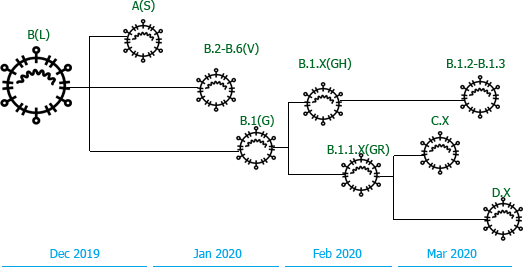
\includegraphics[width=0.8\textwidth]{figures/intro/corona-timeline.png}
        	\captionof{figure}{Schematic representation of the major evolutionary events that gave rise to \acrshort{sarscov2} variants in sequential order (simplified, cf. \cite{jacob2021}). }
        	\label{fig:intro:corona-timeline}
        \end{figure}
        \subsubsection{SARS-CoV-2 variants}
        From approximately summer of 2020 on, \acrshort{sarscov2}'s family tree grew increasingly complex. The main trunk sprouted branches for a number of variants. Gamma, lambda, and mu variants appeared (although none spread worldwide). The tree's canopy was formed by dozens of branches (\cref{fig:intro:nextstrain}).
        \begin{figure}[ht!]
        	\centering
        	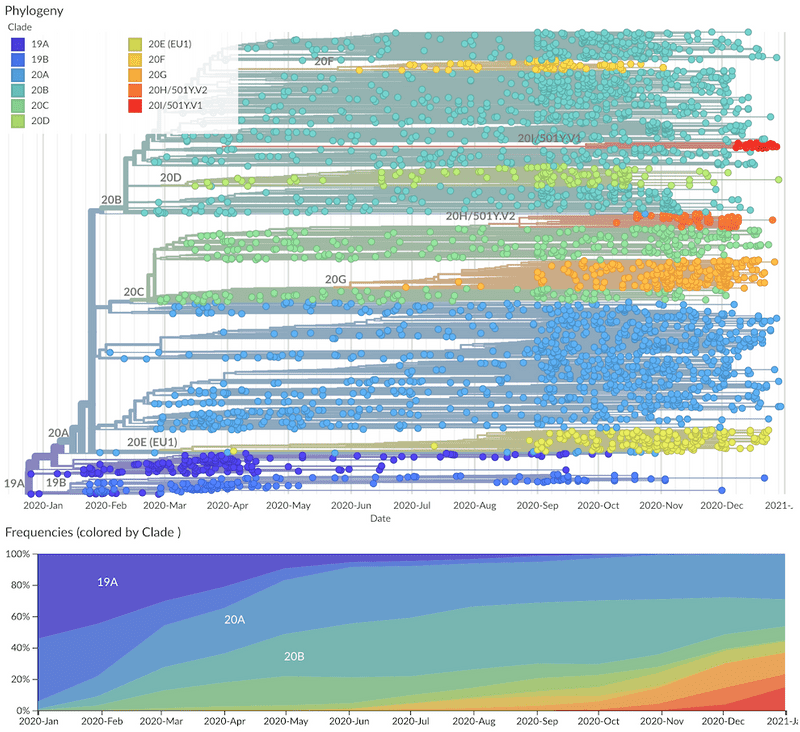
\includegraphics[width=0.8\textwidth]{figures/intro/nextstrain-global.png}
        	\captionof{figure}{\acrshort{sarscov2} phylogenetic tree with a timeline from Nextstrain project labeled by clades (image from \cite{nextstrain2}). }
        	\label{fig:intro:nextstrain}
        \end{figure}
        Researchers track the \acrshort{sarscov2} variants with mutations that are clinically or epidemiologically significant. Detecting variants in a virus usually requires sequencing its complete genome. By sequencing a representative sample of viral specimens in a population, one can determine if new variants are emerging or existing ones are spreading. In particular, variants with the potential or demonstrated ability to be more transmissible, immune evasive, or virulent are closely monitored. These are designated as \acrfull{vois} or \acrfull{vocs}.
        
        On-going pandemic control efforts are challenged by the emergence of \acrshort{sarscov2} variants with greater transmission potential and/or immunity circumvention. In 2020, researchers from South Africa and Great Britain identified two \acrlong{vocs} \cite{voc2022}: alpha and beta \cite{planas2021}. The virus changed rapidly due to these two variants. According to estimates, each variant had around 20 mutations, compared to a few mutations in previous variants. As a result, they became \acrshort{vocs} instead of \acrshort{vois}.
        
        The Delta (B.1.617.2) variant was dominant worldwide between June and December 2021 (\cref{fig:intro:voc-growth}), it has 13 mutations and over 200 known sublineages. Compared to the original virus sequenced in January 2020, the Omicron variant was found to have 50 mutations, when sequenced for the first time in November 2021, and has more than 300 sublineages by now, according to Pango Lineages database \url{https://cov-lineages.org/}. In the middle of 2020, once Omicron's lineage diverged, it became phylogenetically distinct from other known \acrshort{vocs} or \acrshort{vois} \cite{otoole2021}. However, the Omicron variant reached its peak worldwide in January 2022 and continues to be prevalent compared to other variants of concern. 
        
        \begin{figure}[ht!]
            \centering
        	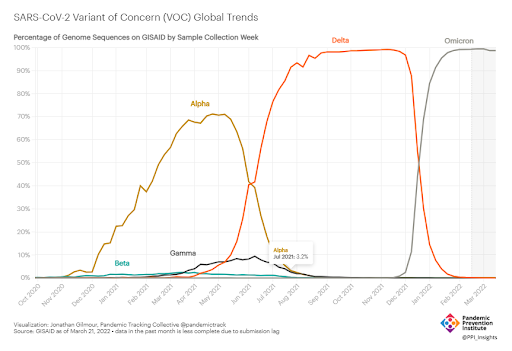
\includegraphics[width=1\textwidth]{figures/intro/voc-growth.png}
        	\captionof{figure}{Chart of global \acrshort{sarscov2} \acrshort{voc} growth from 4 October, 2020, to 21 March, 2022. Graph represents proportions of \acrshort{sarscov2} genome sequences on GISAID by sample collection week per \acrshort{voc} (image from \cite{variants}). }
        	\label{fig:intro:voc-growth}
        \end{figure}
        
        \subsubsection{SARS-CoV-2 naming systems}
        Variants were named with different letters and numbers by different groups of scientists, which can be confusing to the general public. As an example, in the beginning of pandemic, many news organizations and others addressing non-scientific audiences had simplified the naming of variants by referring to the countries in which they first appeared, but this could have resulted in stigma, blame, or prejudice. Therefore, The \acrlong{who} \cite{tracking}, around 2.5 years ago, proposed using Greek alphabet letters to label variants of concern and interest in an effort to make their identification easier to pronounce and less stigmatizing. \acrshort{who} has designated five variants as \acrshort{vocs} and given them the Greek letter names Alpha, Beta, Gamma, Delta, and Omicron (\cref{tab:intro:vocs}).
        
        \begin{table}[ht!]
            \centering
            \small
            \begin{tabular}{lllll}
            \textbf{\acrshort{who}} & \textbf{Pango}               & \textbf{GISAID}    & \textbf{Nextstrain}   & \textbf{Earliest date} \\ \hline
            Alpha                   & B.1.1.7                      & GRY                & 20I (V1)              & September 2020 \\
            Beta                    & B.1.351                      & GH/501Y.V2         & 20H (V2)              & May 2020 \\
            Gamma                   & P.1                          & GR/501Y.V3         & 20J (V3)              & November 2020 \\
            Delta                   & B.1.617.2 and AY Sublineages & G/478K.V1          & 21A,21I,21J           & October 2020 \\
            Omicron                 & B.1.1.529 and BA Sublineages & GR/484A            & 21K,21L,21M           & November 2021\\ \hline
            \end{tabular}
            \caption{Designated \acrlong{vocs} named by different naming systems} \label{tab:intro:vocs}
        \end{table}
        
        Based on genomics experts' rules, several commonly used naming systems \cite{reich} classify the evolving virus forms. The most widely used naming systems are: i) Pango \cite{otoole2021}, which uses the nomenclature system and rules outlined in the publication by A. Rambaut et al. \cite{rambaut2020} and is maintained by the Pango Network (\url{http://pango.network}), and ii) Nextstrain that initially uses 'year-letter' naming. Nextstrain nomenclature was first used to monitor and document the Ebola epidemic in West Africa in 2013-2016 and the Zika outbreak in America in 2018. A number of components make up Nextstrain: Python scripts maintain a database of sequences and metadata, sourced from public databases such as NCBI (\url{www.ncbi.nlm.nih.gov}), GISAID (\url{www.gisaid.org}) and ViPR (\url{www.viprbrc.org}), as well as GitHub repositories and other genomic data sources. There is a suite of tools available for phylodynamic analysis \cite{volz2013}, including subsampling, alignment, phylogenetic inference, and the reconstruction of discrete trait geographic patterns, including the estimation of the probabilities of transmission \cite{hadfield2018}. As soon as \acrshort{sarscov2} genomes are shared, Nextstrain incorporates them and provides analyses and reports once they are available. Nextstrain \acrshort{sarscov2} naming strategy is in sync with Pango. As an example, Nextstrain clade 22A corresponds to Pango lineage BA.4, 22B to BA.5, and 22C to BA.2.12.1 \cite{nextstrain}. There may be some differences in the classification of viruses across or within lineages or clades, although the major lineages and clades are generally assigned in a similar manner.
    
    \subsection{Surveillance of SARS-CoV-2}
    
    In order to respond effectively to \acrshort{sarscov2}, global surveillance is essential for determining which variants require closer monitoring as possible threats to public health. Health professionals and policymakers should have up-to-date information about viral populations present in communities, particularly as new \acrshort{sarscov2} variants emerge that alter viral fitness and/or pathogenesis.
    
    A variety of surveillance techniques are available for \acrshort{sarscov2}. Clinical testing was the most potent and widespread method at the beginning of the pandemic. Different types of clinical testing are possible now. For example, diagnostic testing is one of the clinical testing types and is intended to identify current infections in individuals who have symptoms consonant with \acrshort{covid19} and/or have recently been exposed to \acrshort{sarscov2}. The other type of clinical testing - screening testing - is used for identifying asymptomatic individuals with \acrshort{covid19} cases who don't have known, suspected, or reported exposure to \acrshort{sarscov2} \cite{cdc2020c}.
    
    In addition to clinical testing, public health surveillance entails the systematic collection, analysis, and interpretation of health-related data that are essential for planning, implementing, and evaluating public health practices. An important purpose of surveillance testing in public health is to monitor outbreaks of disease at the community and population level, as well as to characterize disease incidence and prevalence. De-identified specimens are used for surveillance testing, so results are not linked to individuals. To determine if the prevalence of viruses is increasing or decreasing in a particular population, a certain percentage of the population may be sampled for public health surveillance testing \cite{cdc2020c}.
    
    A distinct type of public health surveillance testing is the surveillance of wastewater by high-throughput sequencing. By monitoring wastewater in a community, one can get a better understanding of the types and amounts of viruses and bacteria that are spreading. The virus RNA in stools of people with current or recent \acrshort{sarscov2} infections is detectable in wastewater samples even if they aren't symptomatic. The cost-effectiveness of wastewater sampling comes from the fact that a single sample can reveal information about an entire building, town, or county. It has been suggested that wastewater surveillance could also be used to detect emerging viral variants in an area as they emerge, in addition to tracking \acrshort{sarscov2} transmission levels.
    
    Following subsections will generally discuss the process of lineage identification from isolates with a focus on clinical data surveillance techniques. Starting with extraction approaches (e.g. ampliconic-based, metatranscriptomics, etc.) that are used for the extraction of samples with \acrshort{sarscov2}, sequencing techniques will be described in \cref{sec:intro:virus-identification}. It should be said that talking about extraction methods focus will be done on metatranscriptomics and ampliconic-based approaches because these two library preparation techniques are used more often for \acrshort{sarscov2} datasets, and in this thesis, datasets extracted with the help of these two methods are processed and analyzed. After that, bioinformatics steps of data processing will be discussed. \Cref{sec:intro:clinical-surveillance} will represent existing tracking projects for clinical data surveillance, following by solutions suggested by Galaxy Project for clinical \acrshort{sarscov2} data in \cref{sec:intro:galaxy-effort}.
        
        \subsubsection{Methods of SARS-CoV-2 identification} \label{sec:intro:virus-identification}
    
        \paragraph{Extraction approaches} 
        
        Choosing the most appropriate extraction strategy depends on the final objectives and the type of biological sample. Currently, four different concepts of library preparation have been applied to \acrshort{sarscov2} data: i) shotgun metatranscriptomics, ii) hybrid capture enrichment, iii) amplicon-based, and iv) direct RNA sequencing. To make a comparison between library preparation strategies, \cref{tab:intro:seq-approaches} shows the main characteristics.
        
        \begin{table}[ht!]
            \centering
            \small
            \begin{tblr}{l|llll}
                                     & \textbf{Shotgun}             & \textbf{Amplicon-}    & \textbf{Hybrid}           & \textbf{Direct RNA} \\ 
                                     & \textbf{metatranscriptomics} & \textbf{based}        & \textbf{capture-}         & \textbf{sequencing} \\ 
                                     &                              &                       & \textbf{enrichment}       &  \\ \hline
            Target                   & \acrshort{sarscov2},             &\acrshort{sarscov2}             & \acrshort{sarscov2}               & \acrshort{sarscov2}, \\
                                    & host microbiota,                  & sequence                        & sequence                            & host \\
                                    & host response                     &                               &                                   & transcriptome, \\
                                    &  to infection                     &                               &                                   &  epitranscriptome\\ \hline[dashed]
            Co-infection            &  Yes                              &  No                           &    No/yes (depending              & \\
            detection               &                                   &                               & on gene panel)                    & Yes \\ \hline[dashed]
            Min number of reads     & 20–50 M                           & 5–20 M                        & 5–20 M                            & 0.5 M \\ \hline[dashed]
            Genome Coverage         & 	\begin{math}\geq 99\% \end{math}                 & 	\begin{math}\geq 95-99\% \end{math}          & 	\begin{math}\geq 95-99\% \end{math}              & 	\begin{math}\geq 99\% \end{math} \\ \hline[dashed]
            Accuracy in \acrshort{snv}  & High                          & High                          & Moderate                          & Moderate \\
            identification          &                                   &                               &                                   & \\  \hline[dashed]
            Sample viral load       & <24–28                            & \begin{math}\geq 24-28 \end{math}     & \begin{math}\geq 24-28 \end{math}         & <24–28 \\
            (Ct) requested          &                                   &                               &                                   & \\ 
            (ref Xiao)              &                                   &                               &                                   & \\  \hline[dashed]
            Sample RNA input        & 10–200                            &      	1–50                    &      10–50                        & \begin{math}\geq 1000 \end{math}\\ 
            (ng)                    &                                   &                               &                                   & \\  \hline[dashed]
            Sample type             & Patient                           &      Patient                  &     Patient                       & Viral  \\  
                                    &   specimens                       &      specimens,               &     specimens,                    & cell \\  
                                    &                                   &      environmental            &     environmental                 & cultures \\  
                                    &                                   &       samples                 &      samples                      & \\  \hline[dashed]
            Cost                    &  High                             &       Low                     &       Moderate                    & High \\ \hline[dashed]
            \acrshort{ngs}          & High- or                          &        Mid-                   &    Mid- or                        & \acrshort{ont} \\ 
            platforms               &  ultra high-                      &         throughput            &      high-                        & \\  
                                    &  throughput                       &         platforms             &      throughput                   & \\  
                                    &   platforms                       &                               &      platforms                    & \\  \hline
            \end{tblr}
            \caption{Comparison of \acrshort{sarscov2} library preparation approaches} \label{tab:intro:seq-approaches}
        \end{table}
        
        Most of \acrshort{sarscov2} sequence data is generated using two established library preparation strategies: ampliconic-based sequencing approach and metatranscriptomics sequencing approach. These two approaches will be discussed in more detail in the following two sections. 

        \subparagraph{Metatranscriptomics approach} 
        
        In this method, RNA fragmentation is followed by first- and second-strand cDNA synthesis, and then library preparation is carried out based on the high-throughput sequencing techniques of choice \cite{chiara2020}. Metatranscriptomics technique is able to detect all types of pathogens, which is beneficial. A complete or nearly complete viral genome can be sequenced and reconstructed from available SARS-CoV-2 sequence data that have enough viral loads. However, most preparation protocols involve multiple costly and complicated steps, which inevitably compromises the effectiveness of sequencing of time-sensitive SARS-CoV-2 samples and in identifying other pathogens \cite{meng2021}.
        
        \Cref{fig:intro:metatr-process} shows a simplified schematic representation of the common process for SARS-CoV-2 RNA extraction with metatranscriptomics approach.
        
        \begin{figure}[ht!]
        	\centering
            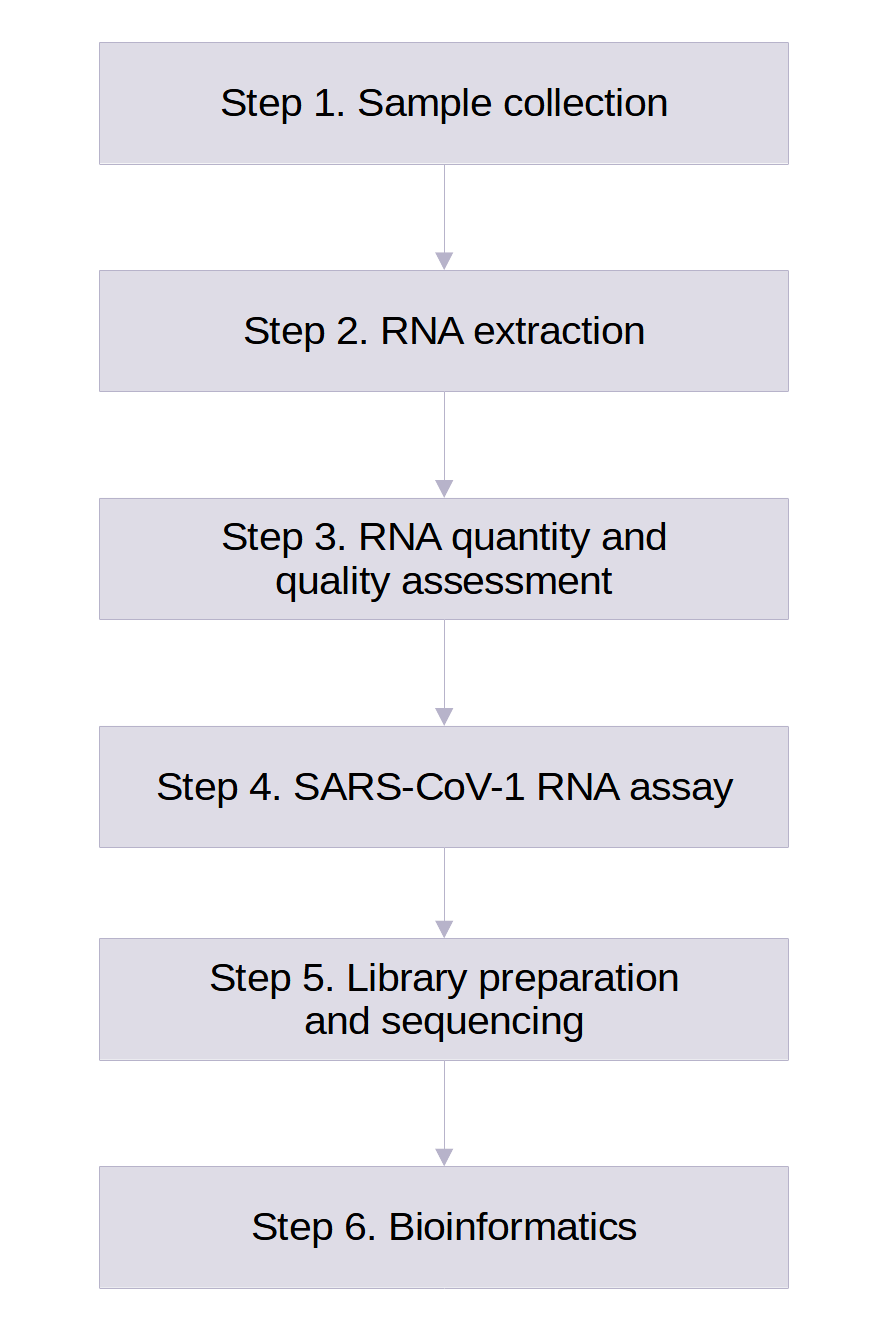
\includegraphics[width=0.5\textwidth]{figures/intro/metatranscriptomics-process.png}
            \captionof{figure}{Schematic representation of the common process for \acrshort{sarscov2} RNA extraction with metatranscriptomics approach (simplified, cf. \cite{chiara2020}). }
            \label{fig:intro:metatr-process}
        \end{figure}
        
        In short, the typical workflow of shotgun metatranscriptomics involves breaking RNA into fragments, synthesizing cDNA from the first and second strands, and preparing a library using the chosen next-generation sequencing technology.

        \subparagraph{Ampliconic approach} 
        
        Amplicon-based method is a highly targeted approach for analyzing genetic variation in specific genomic regions. This extraction method provides information about the targeted sequence. If the targeted sequences are rich in lineage-defining polymorphisms, polymorphisms in the target can be easily linked and lead to easier lineage identification. Deep sequencing of \acrshort{pcr} products (amplicons) facilitates the efficient identification and characterization of variants. Using oligonucleotide probes, regions of interest are targeted and captured. The amplicon-based approach is particularly useful for microbiome samples of diverse origins.

        The use of amplicon sequencing allows researchers to limit the type and number of sequences that can be analyzed. Despite its high specificity, this method requires significant prior knowledge of the sequence that will be 'targeted’. SARS-CoV-2 genome sequencing by amplicon-based methods employs a workflow in which first-strand cDNA is synthesized, followed by multiplex \acrshort{pcr}. Pools of amplicons, covering the entirety or discrete portions of the viral genome, are produced. For SARS-CoV-2, several different multiplex \acrshort{pcr} designs have been proposed, varying in the number and size of amplicons \cite{chiara2020}.
        
        The ARTIC Network's amplicon-based protocol is one of the most widely used SARS-CoV-2 sequencing protocols \cite{lambisia2022,rd2020,rd2022,quick2020} The protocol relies on direct amplification of the virus using tiled, multiplexed primers. This approach has been proven to have high sensitivity and work directly from clinical samples.
        
        The amplicon sequencing approach has several advantages. Through a highly targeted approach, researchers can discover, validate, and screen genetic variants efficiently. High coverage can be achieved by multiplexing hundreds to thousands of amplicons per reaction. The amplicon-based method is able to work with difficult-to-sequence areas. It allows for reducing the cost and time of sequencing compared to other approaches, such as whole-genome shotgun sequencing. But most importantly, it reduces the amount of starting material required. For instance, it is impossible to do non-ampliconic sequencing from nasal swabs, so an ampliconic-based approach should be applied in this case.
        
        In spite of the fact that amplicon sequencing is theoretically convenient and inexpensive, it has some limitations that should be taken into account. As it is stated in a quick guide to tiling amplicon sequencing and downstream bioinformatics analysis \cite{grubaugh2019,loman}, several challenges may arise during the sequencing and analysis process, including contamination, bar-coding issues, and primer binding issues. As a result of the significantly high sensitivity, even a small amount of contaminating templates (such as amplicons from previous work) can lead to the amplification of sequences not present in the sample. The presence of sequences from other samples can confuse the analysis since there is a small rate of barcode "cross-over". Because \acrshort{pcr} relies on synthetic primers, amplicons contain synthetic sequences in their primer binding sites. This is a problem that must be accounted for if the primer sequence contains mismatches compared to the template. Additionally, amplification across the genome can be biased by differences in primer efficiency or possible variations in primer annealing regions. For example, specific genomic regions \cite{itokawa2020} may have less coverage, and/or 3' and 5' untranslated regions may be missed altogether, resulting in incomplete assembly. Due to the fact that the primers are designed using the reference SARS-CoV-2 genome sequence, this approach may not be capable of identifying long structural variants, and high levels of genomic divergence can pose systematic limitations.
        
        A recent study suggests that, although the amplicon-based approach is highly reliable for reconstructing a viral population's most prevalent genome variant, it has a highly biased representation of minor allele frequencies compared to metatranscriptomics experiments conducted on the same samples \cite{xia2020}.
        
        \paragraph{Sequencing techniques}
        
        The majority of \acrshort{sarscov2} sequence data is generated using two sequencing platforms: \acrfull{illumina} and \acrfull{ont}. 
        
        \subparagraph{\acrshort{illumina} sequencing}
        
        \acrshort{illumina} sequencing, second-generation sequencing, detects the sequence of RNA by using reversible dye terminators technology. Solexa company, now part of Illumina company, invented the reversible dye terminators technology and engineered polymerases that are used in this sequencing method.
        
        \acrshort{illumina} sequencing begins with the cleavage of the sample into short sections.  A short read or fragment of 100-150bp is created at the start of the \acrshort{illumina} sequencing process. The fragments are then ligated to generic adaptors and annealed to slides. Each fragment is amplified by \acrfull{pcr}. By doing this, the same fragment appears in many copies. Sequencing slides contain fluorescently labeled nucleotides, RNA polymerase, and terminator molecules. As a result of the terminator, only one base is added at a time. It allows the next base to be added to the site after each cycle terminator is removed. In each cycle, the computer detects the base added by relying on fluorescent signals \cite{difference2021}. 
        
        \subparagraph{Nanopore sequencing}
        
        \acrshort{nanopore} sequencing is third-generation sequencing technique that detects the RNA sequence by using a protein nanopore. \acrshort{nanopore} sequencing involves RNA passing through a nanopore and changing its current. There is a relationship between the size, shape, and length of the RNA sequence and how a current changes. In order to obtain the specific RNA sequence, the resultant signal needs to be decoded. There is no need to modify nucleotides, and the method works in real-time.
        
        A number of nanopore sequencing devices are manufactured by \acrlong{ont}. Flow cells are a common feature of \acrshort{nanopore} sequencing devices. An electro-resistant membrane surrounds a number of tiny nanopores in this flow cell. Each nanopore corresponds to its own electrode. An electrode connects to a sensor chip and a channel. A nanopore's electric current is measured by this electrode. As molecules pass through nanopores, their current is changed or disrupted. A characteristic squiggle results from this disruption. Squiggles are decoded in real-time to determine RNA sequences \cite{difference2021}. 
        
        \subparagraph{Comparison of \acrshort{nanopore} and \acrshort{illumina}} 
        \acrshort{nanopore} sequencing uses a nanopore to detect the RNA sequence, while \acrshort{illumina} sequencing technique uses reversible dye terminators technology to detect the sequence of RNA. Both techniques have markedly high accuracy. More precisely, \acrshort{nanopore} sequencing has 92-97\% accuracy, while \acrshort{illumina} sequencing has 99\% accuracy. The following \cref{tab:intro:ont-vs-illumina} lists the differences between \acrshort{nanopore} and \acrshort{illumina} sequencing.
        
        \begin{table}[ht!]
            \centering
            \small
            \begin{tblr}{l|ll}
                                        & \textbf{\acrshort{nanopore}}                   & \textbf{\acrshort{illumina}} \\       \hline
            \textbf{Generation}         & third-generation                                 & second-generation \\                         \hline[dashed]
            \textbf{Founded by}         & Prof. David Deamer                        & Prof. Shankar Balasubramanian \\
                                        &                                           & and Sir David Klenerman \\            \hline[dashed]
            \textbf{Accuracy}           & 92-97\%                                   & 99\% \\                               \hline[dashed]
            \textbf{Long/short read}    & long reads                                & short reads \\                        
            \textbf{sequencing}         &                                           &  \\                                   \hline[dashed]           
            \textbf{Read length}        & 2,272,580 bp                              & 75-300 bp \\                          \hline[dashed]
            \textbf{Time taken}         & Real time                                 & 4 to 56 h \\                          \hline[dashed]
            \textbf{Cost}               & \$7-100                                   & \$5-150 \\                            \hline[dashed]
            \textbf{Advantages}         & longest individual reads                  & potential for high sequence yield \\  \hline[dashed]
            \textbf{Disadvantages}      & lower throughput than other machines      & expensive \\                          \hline
            \end{tblr}
            \caption{Comparison of \acrfull{nanopore} and \acrfull{illumina} sequencing} \label{tab:intro:ont-vs-illumina}
        \end{table}

        \paragraph{Data processing with bioinformatics methods} 
        
        For the next stage after sequencing, bioinformatics analysis should be executed. Tools can differ from one pipeline to another. But the main steps, in general, are more or less the same. After getting raw data reads, they have to be processed with different steps. 

        Quality control step is often used because there is no perfect sequencing technology, and each instrument will generate different types and amounts of errors, such as incorrect nucleotide calls. Each sequencing platform has technical limitations that result in these incorrectly called bases. Thus, it is important to identify and exclude error types that may affect downstream analysis interpretation. As a result, sequence quality control is an essential first step in the analysis process. 
        
        Another step, primer trimming, is a specific step for datasets generated with ARTIC protocol. The auxiliary file is used for this step - a \acrshort{bed} file specifying the primers used during amplification and their binding sites on the viral genome. Primer trimmer uses primer positions supplied in a \acrshort{bed} file to soft clip primer sequences from an aligned and sorted \acrshort{bam} file. Following this, the reads are trimmed based on a quality threshold. More specifically, some primer trimmers, in order to do quality trimming, use a sliding window approach. The window slides from the 5' end to the 3' end and if at any point the average base quality in the window falls below the threshold, the remaining read is softly clipped. If after trimming, the length of the read is greater than the minimum length specified, the read is written to the new trimmed \acrshort{bam} file. It should be noted, for datasets that were not generated with primer-based protocol like ARTIC, this primer-trimming step is not applicable.
        
        Moreover, adapter trimming step is processed. For instance, upon Illumina sequencing we receive raw reads with adapters at 3’ end. The adapters contain the sequencing primer binding sites, the index sequences, and the sites that allow library fragments to attach to the flow cell lawn. This might influence a downstream analysis, thus, adapter trimming is required. 
        
        A decontamination step can then be included to remove reads from the human genome, since viral sequence data from clinical samples commonly contain human contamination. Prior to sharing, it needs to be removed for legal and ethical reasons as well as to speed up downstream analysis \cite{hunt2022}.
        
        The crucial step is mapping with reference SARS-CoV-2 sequence \emph{NC\_045512.2} that is publicly available in NCBI database \cite{genome2020}. A mapping tool of choice can differ from one pipeline to another, depending on read length, sequencing technology, and other factors. 
        
        Some pipeline steps are not always included in pipelines, such as removing duplicates. This step can be important for Illumina sequencing reads. During the sequencing process with Illumina sequencing technology, some duplicate reads/sequences can be produced, which can create bias in downstream analyses. It is, therefore, possible to remove duplicates or mark them without removing them. When removing duplicates, one should be certain that they are duplicates and not repeated regions. It can therefore be reasonable to keep duplicates marked rather than remove them, as this can be useful for downstream analysis.
        
        Another step, which is not present everywhere, is helpful due to potential ambiguity, while indels are not parsed when they overlap the beginning or end of alignment boundaries. Input insertions and deletions must be homogenized with left realignment in order to gain a more homogeneous distribution. Left realignment will place all indels in homopolymer and microsatellite repeats at the same position, provided that doing so does not introduce mismatches between the read and reference other than the indel \cite{garrison2012}. Basically, this step is considered to correct mapping errors and prepare reads for further variant calling.
        
        Additionally, realigned reads can be taken and checked for the quality of alignment using bioinformatics tools (e.g., Qualimap \cite{qualimap,qualimap2}). Based on the features of the mapped reads, it analyzes \acrshort{sam}/\acrshort{bam} alignment data and provides a global picture of the data that can help detect biases in sequencing and/or mapping of the data and ease decision-making for further analysis.
        
        After mapping and other additional preparation steps, variant calling should be run where variants from sequence data are identified. Variant calling step is followed by mutation annotation where \acrshort{vcf} file is used as input and annotated SARS-COV-2 genome - as database, and it is transformed to \acrshort{maf} format. The data is not changed; here, only format is changed to be more readable.

        There is a number of publications describing different combinations of bioinformatics steps and tools used to process and analyze raw data \cite{baker2020} and ranging from transparent to opaque \cite{holshue2020}. Analytical transparency is crucial for such cases. Now, many organizations provide transparency to data processing and analyzing approaches. For example, the COG-UK datasets, protocols, methods, and techniques for collecting and preparing SARS-CoV-2 virus samples for sequencing, as well as short-read and long-read sequencing, are all publicly available \cite{quick2020}.
        
        \subsubsection{SARS-CoV-2 tracking projects} \label{sec:intro:clinical-surveillance}
        
        \acrshort{sarscov2} variants began being tracked from the beginning of the \acrshort{covid19} pandemic in order to observe global trends of \acrfull{vocs} (\cref{fig:intro:voc-growth}).
     
        In the course of the \acrshort{covid19} pandemic, many laboratories have developed genomic epidemiology data infrastructures. By January 2022, there were nearly 4000 unique labs submitting data to the GISAID EpiCoV database. A consortium called COG-UK \cite{cogconsortium} is one of the well-known \acrshort{sarscov2} tracking projects. Their research built on the availability of \acrshort{sarscov2} genomes generated throughout the pandemic and spanned across variants, data linkage, and quality. Moreover, there are other complementary projects focused on the emergence of \acrshort{sarscov2} variants. At the beginning of the \acrshort{covid19} pandemic, a problem with available data to analyze occurred \cite{baker2020}. In this regard, COG-UK is the \acrshort{sarscov2} data tracking project that reflected quickly to that and was one of the first that shared data for publicity. Another example of a tracking project that is focused on \acrshort{sarscov2} sequencing is the Swiss \acrshort{sarscov2} Sequencing Consortium (S3C) \cite{chen2022,swiss}.
        
        Currently, large amounts of sequencing data have become increasingly available and must be constantly analyzed. As a result of these data, one can monitor the emergence and spread of new variants, as well as understand the viral evolution dynamics. Nevertheless, transparent and freely available infrastructure for such analysis is not present everywhere. It is often the case that infectious disease outbreaks occur in remote areas without adequate infrastructure or in political situations that make unbiased interpretation of results impossible. In response, there is a need for free, open, and robust analytical approaches accessible to everyone worldwide for data analysis, interpretation, and sharing.

        \subsubsection{Galaxy effort to surveillance data processing} \label{sec:intro:galaxy-effort}
        
        In order to address global health emergencies in an accessible and transparent manner, there is a need for scientific computing infrastructure to help bridge these gaps. Data and data analysis transparency were the primary focus of the Galaxy effort.

        Through its graphical web interface, Galaxy allows users to use tools from a variety of domains for \acrshort{fair} \cite{wilkinson2016} data analysis; run code in interactive environments (RStudio, Jupyter, etc.) along with other tools or workflows; manage data by sharing and publishing results, workflows, and visualizations; ensure reproducibility by capturing information that allows data analysis to be repeated and understood \cite{baker2020}.
        
        Galaxy offers powerful public computational infrastructures designed specifically for research purposes in the United States, the European Union, and Australia. In the United States, there is the XSEDE \cite{towns2014} consortium; in the European Union, there is the deNBI \cite{elixirde} and ELIXIR \cite{elixir2,elixir} consortiums; and in Australia, there is the Nectar Cloud consortium. Due to their global accessibility, support for diverse configuration schemes (from traditional computational clusters to fully virtualized cloud-like setups), and ability to provide cutting-edge hardware, large-scale public computing resources are well suited to tackling the bioinformatics challenges of the current pandemic. 
        
        In combination with open-source software tools, this public computational infrastructure offers a complete solution to the SARS-CoV-2 data analytics challenge. Galaxy provides a glue to bind these into a unified analytics platform that manages users, allocates storage, and pairs analysis tools with computational resources fluidly. The platform provides both a graphical user interface and programmatic access in order to accommodate researchers with different degrees of computational expertise. 

        \paragraph{Four SARS-CoV-2 analysis workflows} 
        
        Based on Galaxy, four workflows were developed aimed at detecting and interpreting sequence variants in SARS-CoV-2 in clinical data. A special webpage was created to track Galaxy efforts on SARS-CoV-2 analysis, workflows, data, and documentation \cite{galaxyproject}. These workflows can be accessed immediately and freely in three global Galaxy instances: in the United States (\url{https://usegalaxy.org/}), the European Union (\url{https://usegalaxy.eu/}), and Australia (\url{https://usegalaxy.org.au/}). 
        
        When creating workflows for SARS-CoV-2 analysis, W. Maier et al. \cite{maier2021b} took several goals into account. They aimed to provide continuous analysis of within-host sequence variants in high-quality public read-level databases. The other goal was to provide maintenance of curated workflows for the analysis of SARS-CoV-2 sequence data and free powerful infrastructure to execute them, such as Galaxy infrastructure. They developed a continuously updated analysis page and dashboard summarizing the latest insights from the variant. Last but not least focus was to provide access to all results in raw and aggregated form for immediate use.
        
        As suggested by W. Maier and colleagues, SARS-CoV-2 clinical data analysis is organized into two stages of analysis (\cref{fig:intro:galaxy-effort}). Stage 1 takes raw sequencing data as input and produces intermediate summaries such as allelic variants and annotations in mutation annotation format (\acrshort{maf} files) and variant calling format (\acrshort{vcf} files). Basically, at Stage 1, depending on library preparation and data sequencing method, the appropriate workflow is taken. Thereby, for datasets prepared by using ARTIC amplicon-based protocol, two workflows are available: for datasets sequenced with \acrfull{ont} and \acrfull{illumina}. As for datasets prepared with metatranscriptomic protocol, there are two workflows available for Illumina-based sequencing technology. The difference is in the types of reads obtained. One workflow works with paired-end reads, while another one works with single-end reads.
        
        Interpreting and visualizing the Stage 1 outputs are the focus of Stage 2. Additional reporting workflow is developed to analyze outputs of Stage 1, which generates tabular and \acrshort{json} files. These files serve as input for analysis based on two software systems, Jupyter, and ObservableHQ, for visualizing results.
        
        \begin{figure}[ht!]
        	\centering
            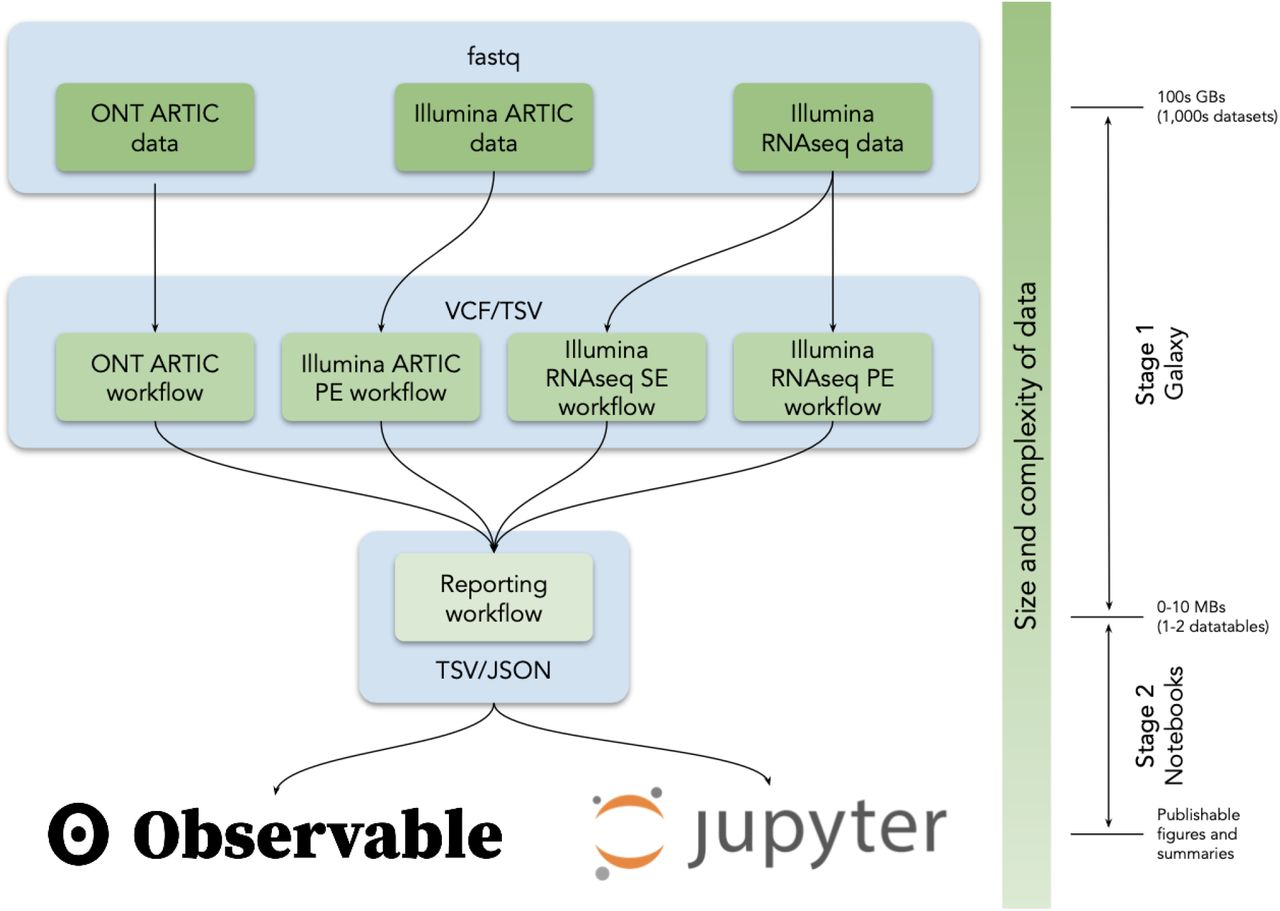
\includegraphics[width=0.7\textwidth]{figures/intro/galaxy-analysis.jpg}
            \captionof{figure}{Analysis flow in the analysis system suggested by GalaxyProject (image from \cite{maier2021b}). }
            \label{fig:intro:galaxy-effort}
        \end{figure}
        
        The choice of bioinformatics tools for these four workflows is made based on the method of sequencing and the type of data obtained by the method. For paired-end reads, the BWA-MEM \cite{li2013,burrows} mapper is used to map to the SARS-CoV-2 sequence. Bowtie2 \cite{ultrafast,langmead2012} mapper is used for single-end read datasets sequenced with Illumina method, whereas minimap2 \cite{burrows,li2018} mapper is most appropriate for datasets sequenced by Oxford Nanopore since Oxford Nanopore sequencer generates very long reads with many errors. As for variant caller, LoFreq is used in all four workflows since it is known as a more ultra-sensitive variant caller for uncovering cell-population heterogeneity \cite{lofreq}.

        \paragraph{Bots for automated SARS-CoV-2 surveillance } 
        
        Additionally, Galaxy team has developed bots to assist in SARS-CoV-2 surveillance \cite{bots2022}, a viable tool for automating the analysis of a large number of SARS-CoV-2 sequences regularly. In essence, it is a set of automation scripts that can be integrated into any scheduling system with a daily throughput of around 1000 samples on a Galaxy instance. Galaxy bots allow to upload newly available data, start a variation analysis workflow, and follow up with downstream workflows for consensus building and reporting once the variation analysis is complete. It is possible to use bots for SARS-CoV-2 surveillance to track National Genome Surveillance projects, such as COG-UK, and reanalyze their data as it becomes available. These scripts are a decent automated sequence data analysis pipeline that works with two Galaxy SARS-CoV-2 surveillance workflows for datasets extracted with ARTIC protocol. 
        
        Galaxy workflows developed for SARS-CoV-2 clinical surveillance have shown adequate results. There are, however, some limitations. Currently, Galaxy workflows do not focus on wastewater surveillance. Thus, Galaxy workflows can be improved and repurposed to improve SARS-CoV-2 wastewater surveillance. The current thesis attempts to focus on it.

        \subsection{Wastewater surveillance}
        
        This section will provide the introduction to wastewater surveillance in general and particularly for SARS-CoV-2 as well as show the limitations and benefits of wastewater surveillance over clinical surveillance. Then, the focus will be on wastewater surveillance contribution to global safety and global efforts towards it. After that, a few words about the wastewater surveillance working groups will be said. 
        
        Wastewater surveillance has played an important role in controlling outbreaks, for example,  poliovirus outbreaks which have been challenging in the past. Israel detected wild poliovirus in wastewater samples between 2013 and 2014, 25 years after the last case. In March 2022, poliovirus was found in sewage samples from Jerusalem and surrounding areas. Both outbreaks were contained with vaccination campaigns, which prevented the further spread of the virus. There was only one case of paralysis in an unvaccinated child in 2022, and no cases of paralysis occurred in the 2013–2014 outbreak in Israel due to rapid detection enabled by wastewater surveillance. In recent two years, increased public awareness of any suspicious virus, including poliovirus, and ubiquitous usage of wastewater surveillance of poliovirus are preventing any cases of paralysis following the recent re-emergence of polio in New York \cite{russo2022}.  
        
        With the experience in poliovirus wastewater surveillance, it was reasonable to use this method for other virus surveillance. People who are infected with SARS-CoV-2 have the virus in their stools regardless of whether they show symptoms of the disease. Additionally, SARS-CoV-2 RNA may be carried into the sewer system from urine  \cite{chan2021} and respiratory secretions (from hand washing, showering, nasal lavages, tissues, and sputum), as indicated by detected SARS-CoV-2 RNAs in washbasins and shower siphons \cite{dohla2022}.  
        
        Wastewater with these secrets inevitably ends up in wastewater treatment plants where samples can be collected. In treatment plants, typically, samples of incoming sewage at an early stage are taken, and the plants are designed so that this can be done safely and effectively \cite{foladori2020}. The automated sampling system can also be used to collect wastewater samples directly from pumping stations or at suspected virus hotspots such as hospitals \cite{wang2020}, dormitories, residential districts, or confined spaces like cruise ships or passenger airplanes \cite{ahmed2020}. 
        
        During a pandemic such as COVID-19, wastewater surveillance \cite{new2022,schmidt2020} can be used to detect both the presence and absence of the virus, as well as the emergence and transmission of new variants that are more infectious or immune-evading. There will be more SARS-CoV-2 variants, regardless of when or where the next major variant emerges. It is imperative to detect them as soon as possible, whether they originate from known variants or appear independently \cite{wastewater2022}.  
        
        A method of wastewater genomic surveillance was used by California researchers to detect SARS-CoV-2 infections on the campus of the University of California, San Diego (UCSD), in the midst of the pandemic during a period of 10 months. Researchers found that their approach was effective in identifying viral variants of concern as early as two weeks before they showed up in clinical tests, according to an article published in Nature \cite{karthikeyan2022}. Additionally, wastewater samples were analyzed in Sweden. The Rya wastewater treatment plant in Sweden collected samples of wastewater from Gothenburg and surrounding municipalities from mid-February to June 2020. It appeared that the amount of SARS-CoV-2 varied with peaks roughly every four weeks, preceding variations in the number of newly hospitalized patients by 19-21 days \cite{saguti2021}. 

        The SARS-CoV-2 virus is already tracked by wastewater surveillance in over 55 countries [80], and various monitoring programs are run worldwide. In the US, in September 2020, the Centers for Disease Control and Prevention (CDC) launched a National Wastewater Surveillance System \cite{cdc2022b} in conjunction with health departments across the country. SARS-CoV-2 levels in community wastewater are monitored by this program. 

        \subsubsection{Challenges and limitations of wastewater surveillance over clinical surveillance} 
        
        In spite of the increasing popularity of wastewater surveillance across the world, it can be more challenging to detect viruses accurately in wastewater, compared to clinical testing \cite{farkas2020}. Prior to virus concentration, large quantities of sewage sludge typically should be filtered to remove debris, flocculated, precipitated, or centrifuged. Molecular analyses, like \acrshort{pcr}, can be hindered by concentration techniques that damage genomic material. Furthermore, sewage contains a wide variety of other microbes and viruses, which may produce false positive results, as well as human DNA \cite{wastewater2022}. 
        
        Because it contains human DNA, wastewater data need to be anonymized due to privacy concerns. However,  pathogenic surveillance has the task of linking genetic information with the clinical manifestations and immunological status of patients [85]. That means that wastewater surveillance is limited in this regard, and it is able to provide only coarse population-level information.
        
        Another challenge is a great deal of variation in how much virus is shed in feces and urine between individuals, so it is very difficult to quantify the number of people who are infected \cite{farkas2020}.
         
        Moreover, due to the mobility of populations in any particular region, wastewater surveillance cannot pinpoint infected individuals or trace transmission. As a result, wastewater detection efforts can be hindered by unwittingly spreading a pathogen by infected people passing through a region, often after the index case has moved on \cite{ahmed2022}. 

        \subsubsection{Benefits of wastewater surveillance over clinical surveillance} 
        
        Nevertheless, the use of wastewater methods is quite beneficial, since they can allow the detection of outbreaks before the first positive clinical tests are reported. Based on the first cases of SARS-CoV-2 wastewater surveillance, it has already been found \cite{zhang2021} that virus RNA is detected in sewage even when COVID-19 prevalence is low, and that the correlation between concentration in sewage and reported COVID-19 prevalence indicates that sewage surveillance can be used as a sensitive tool to monitor viral circulation in the population.
         
        Likewise, wastewater surveillance is more economical than clinical testing since it can screen large numbers of people with just a few samples and does not need clinician involvement.
        
        Another advantage is that by using the wastewater surveillance of SARS-CoV-2 method, data can be collected from people who do not have access to healthcare or in places, so-called “sequencing deserts”, around the world where sequencing capacity is limited. Among such "sequencing deserts'', new, potentially dangerous variants, like Omicron, are able to emerge and spread undetected. There is a risk that new variants or subvariants will emerge until representative samples are sufficiently sequenced. Wastewater surveillance is one of the opportunities for covering 'sequencing deserts' for surveillance of variants of SARS-CoV-2. As a result, a very close to a real-time overview of disease prevalence could be provided since it was proved \cite{zhang2021} successful enough in revealing infection dynamics earlier than clinical testing. In \cref{fig:intro:ww-process}, the schematic diagram shows the process of detecting viruses by wastewater surveillance against clinical surveillance. 
        \begin{figure}[ht!]
        	\centering
            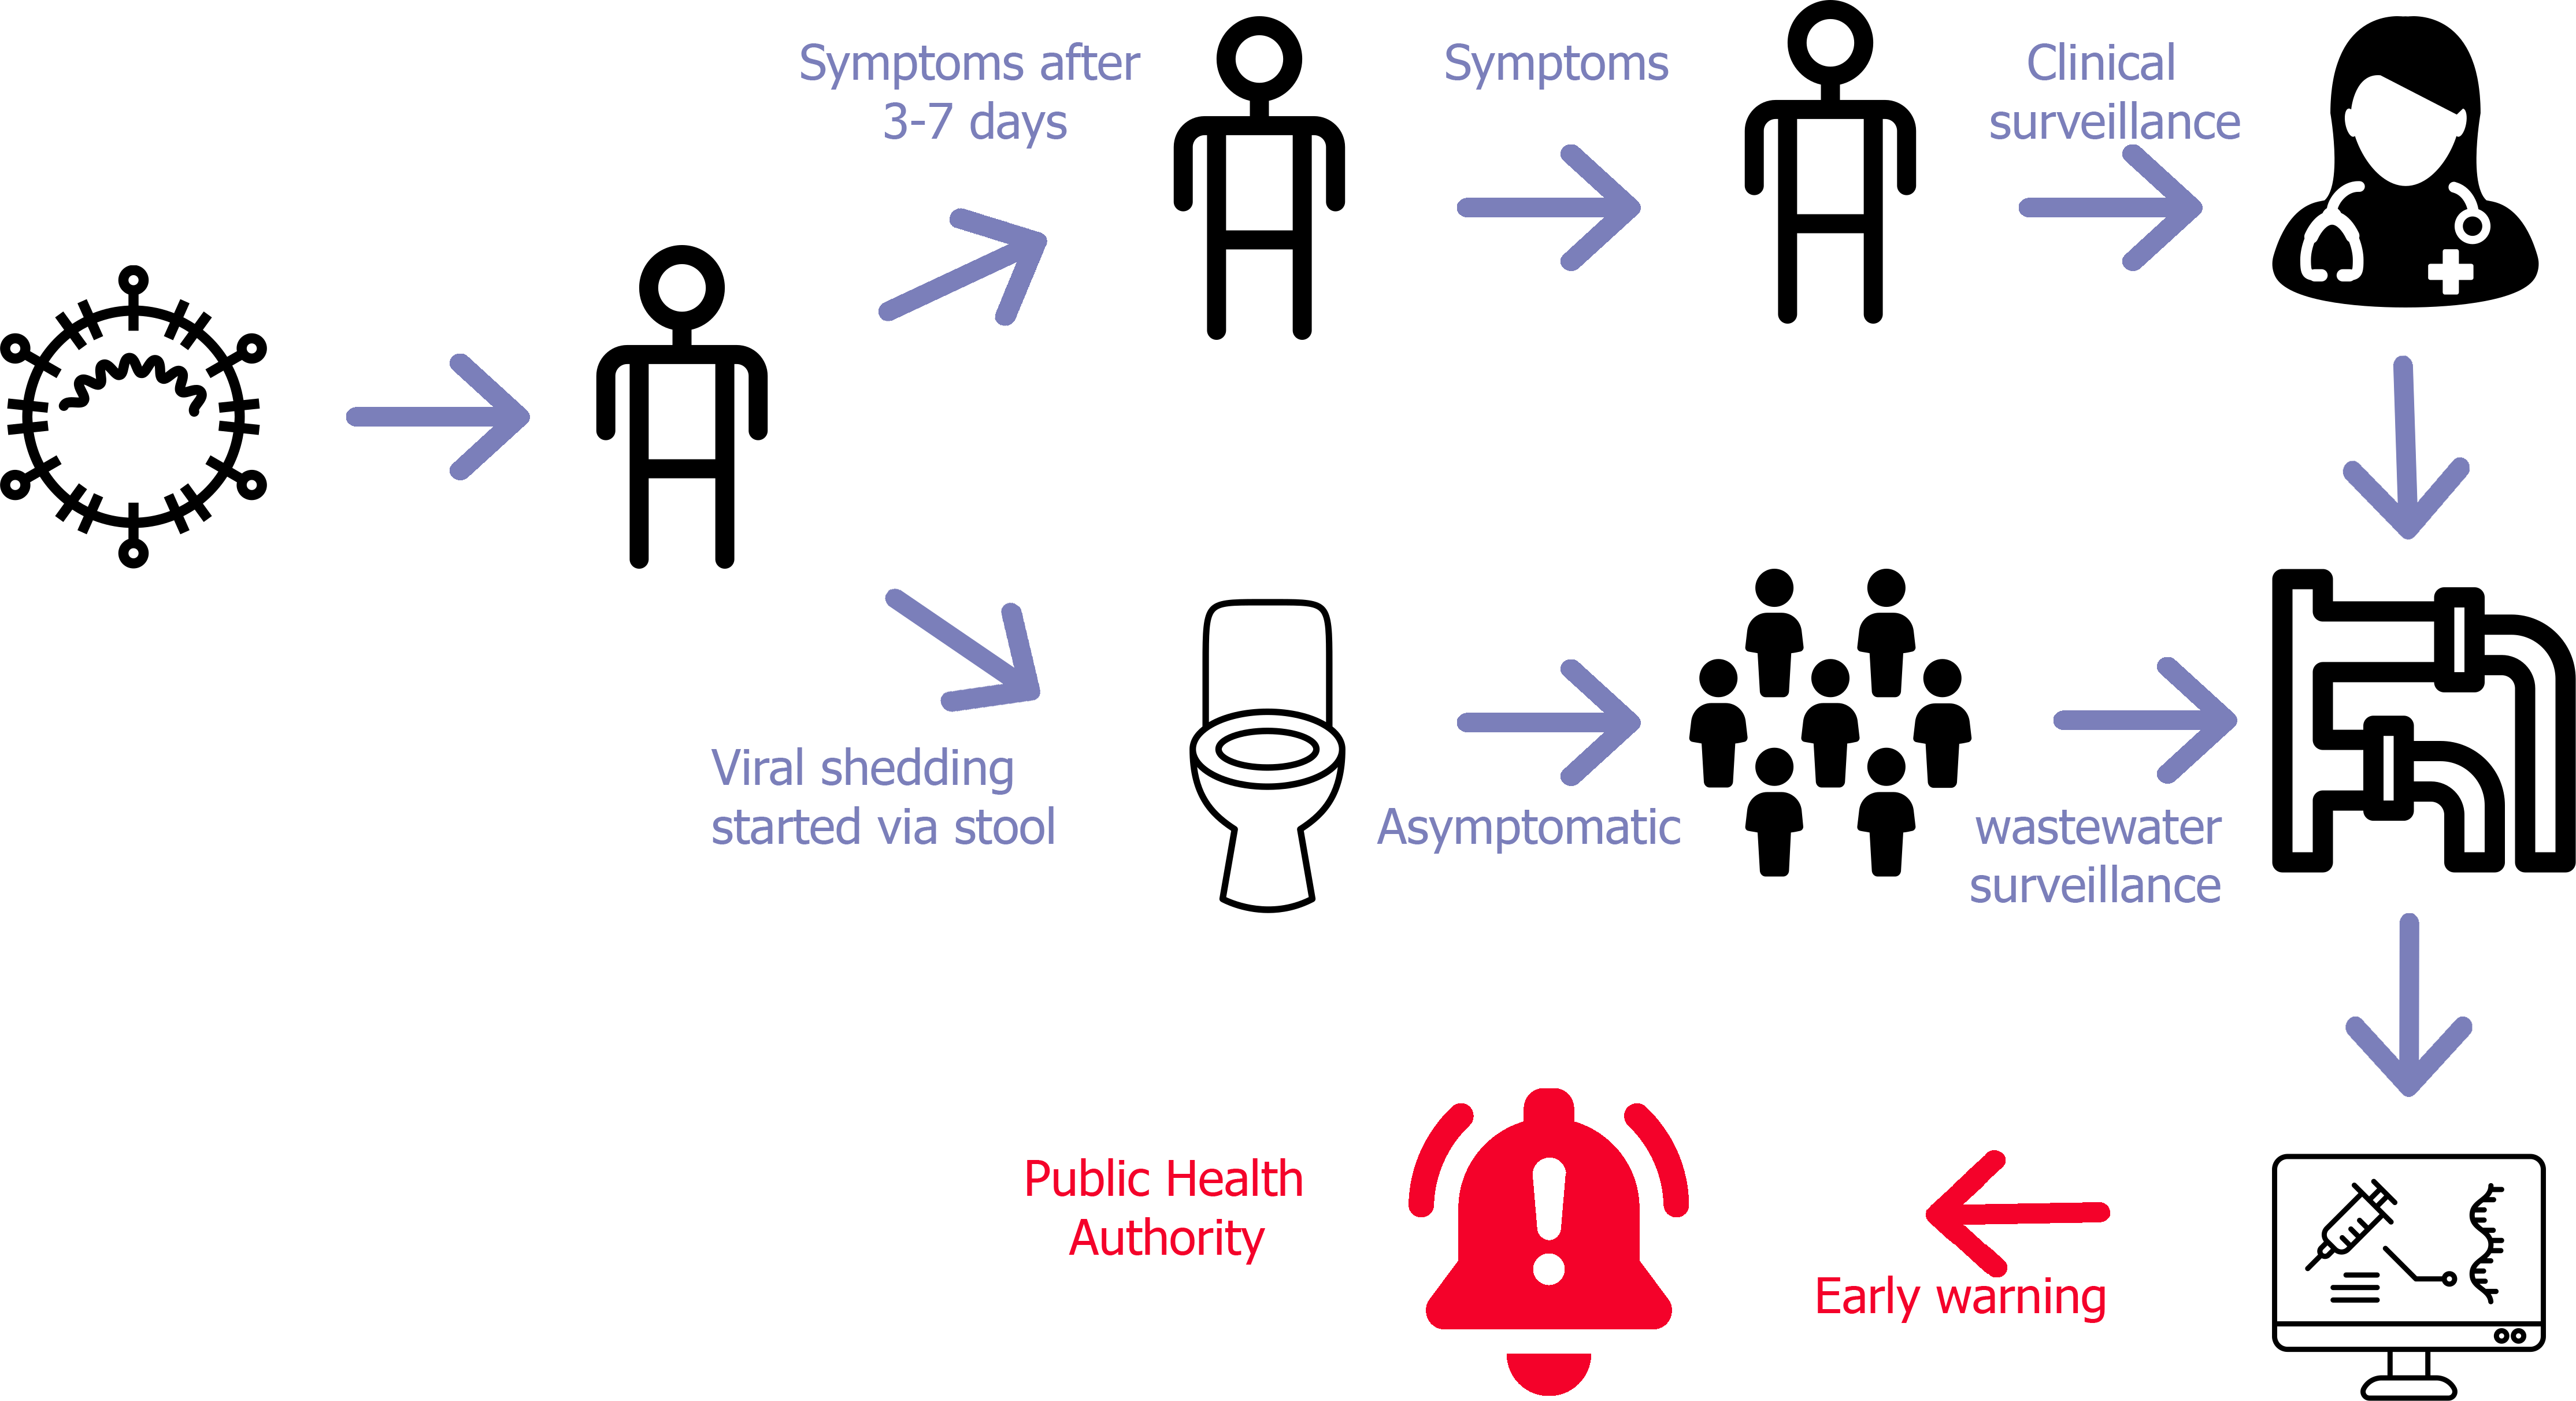
\includegraphics[width=0.9\textwidth]{figures/intro/ww-process-v2.png}
            \captionof{figure}{Schematic diagram shows the process of detecting viruses by wastewater surveillance against clinical surveillance.}
            \label{fig:intro:ww-process}
        \end{figure}

        \subsubsection{Wastewater surveillance contribution to global safety} 
        
        Viruses are not the only thing that can be monitored in wastewater. This method can be used to detect other microbial pathogens \cite{ko2022}, antimicrobial resistance \cite{hendriksen2019}, or chemical water contaminants \cite{jung2020}. Further, these tools can be used on samples from other settings, such as transport hubs, hospitals, schools, workplaces, and leisure facilities, in addition to wastewater treatment facilities. Besides public-health applications, wastewater surveillance data may be useful to researchers examining community trends and the efficiency of health policies and non-pharmaceutical interventions \cite{wastewater2022}. 
        
        Wastewater surveillance provides valuable information on epidemiological developments at the population level that complements case-based surveillance and aids in resource allocation. Likewise, this can be applied to a global scale. Using the wastewater-based epidemiology method, places and communities with poor healthcare accessibility can shed light on the blind spots of pathogen surveillance. A wastewater surveillance system for infectious diseases could contribute to global safety if it is carefully set up and used in a respectful manner.

        The wastewater surveillance methods seem to fit the bill for enabling early, economical, and efficient detection so that public-health measures can be implemented as soon as they are necessary. Globally, wastewater surveillance is poised to become part of public health strategies \cite{hendriksen2019}. 

        \subsubsection{Global effort to wastewater surveillance} 
        
        Enough efforts have already been made in this direction in the world. Various wastewater tracking projects took place in countries like Estonia \cite{detecting2022,reoveeseire}, Greece \cite{ismart}, and Canada \cite{coalition}. As a result, COVID-19 trends are visualized within the sewer community, contributing to COVID-19 incidence (both reported and unreported). In response to the COVID-19 pandemic, wastewater surveillance data are used to understand and act, and in public health decision-making. \href{https://www.arcgis.com/apps/dashboards/c778145ea5bb4daeb58d31afee389082}{COVIDPoops19}, a dashboard developed by Colleen Naughton and colleagues at the University of California (UC), Merced, shows monitoring projects for SARS-CoV-2 have sprung up in at least 70 countries since then \cite{naughton2021}. By October 2021, the European Union recommended that all member countries establish monitoring systems for SARS-CoV-2. 26 of 27 countries have adopted this recommendation. In the United States, the National Wastewater Surveillance System includes 400 sites in 19 states. In the U.S., on 2 March 2022, President Joe Biden's administration said the monitoring system would be part of efforts to detect new variants as the Centers for Disease Control and Prevention added a national dashboard of wastewater data. As well, there is a successful project in Bengaluru that has been expanded to half a dozen other cities in India \cite{pandemic2022}. 
        
        At the same time, there are several initiatives to coordinate wastewater surveillance efforts via working groups. For example, 219-nCoV \acrshort{wbe} is a Slack space in which worldwide participants share protocols, publications, and other state-of-the-art resources, and help each other. At the European level, a focus group meets every month for wastewater surveillance efforts coordination.
        
    \subsection{Motivation and the goal of the thesis}
    As a result of extensive global efforts, numerous pipeline solutions have already been proposed by the scientific community. In terms of accessibility and readiness for use, wastewater surveillance pipelines exist with some limitations. Some pipelines demand an upstream set of tools or sub-pipelines that can take some time to prepare datasets. In addition, they are quite strict when it comes to the tools they use. The best performance is achieved by combining different tools in different workflows. Furthermore, the reproducibility of these workflows is not straightforward. Researchers typically receive instructions of varying depths of detail explaining how to launch workflows in their environments. When comes to repeat analysis several times, can turn to some inconveniences. Additionally, researchers are not provided resources to conduct these workflows and downstream analyses afterward. The platform and resources are crucial to research, even though they are a second priority to some scientists.

    In this master thesis, I aim to provide a complete workflow based on Galaxy that assists platforms that can ensure data analysis transparency and reproducibility. To be precise, I intend to adapt the Galaxy workflows developed for clinical data to process wastewater data. In doing so, I integrate existing tools, test these workflows on mock datasets as well as real datasets, and benchmark them against each other and with other solution offered by other researchers.
    
     






%%%%%%%%%%%%%%%%%%%%%%%%%%%%%%%%%%%%%%%%%%
% Master Thesis 
% Polina Polunina
% November 2022 
%
% License:
% CC-BY-SA 4.0 -- Creative Commons Attribution-ShareAlike 4.0 International
% https://creativecommons.org/licenses/by-sa/4.0/legalcode
%%%%%%%%%%%%%%%%%%%%%%%%%%%%%%%%%%%%%%%%%%
\section{State-of-the-art}

From the beginning of the COVID-19 pandemic, several approaches have been presented to determine SARS-CoV-2 in wastewater samples. An overview of existing tools and pipelines will be given in \cref{sec:prior:methods}. Some tools and pipelines aiming to detect SARS-CoV-2 lineages and their abundance in wastewater samples will be considered. More specifically, \cref{sec:prior:methods:tools} will show individual tools that need to be implemented into pipelines, while \cref{sec:prior:methods:pipelines} will demonstrate standalone pipelines for detecting lineages and their abundances. In \cref{sec:prior:methods:comparison} an overview of the comparisons will be presented both for individual tools and for standalone pipelines. In \cref{sec:prior:discussion}, a short discussion of the existing methods with respect to the goals of this thesis will be given.

    \subsection{Methods for wastewater surveillance} \label{sec:prior:methods}
    Existing methods for SARS-CoV-2 wastewater surveillance differ. Some approaches present individual tools that require data preprocessing and/or need to be plugged into pipelines before they can be used, while another methods offer independent pipelines that do all the analysis from raw data to determining lineages and their abundances. This determination can be focused on \acrfull{vocs} as well as \acrfull{vois} and additionally with an intention to detect newly appeared unknown variants. Both types of methods will be discussed in the following sections.
    
        \subsubsection{Individual tools} \label{sec:prior:methods:tools}
        Methods that offer individual tools to discern SARS-CoV-2 lineages and their abundances take preprocessed data. Raw data needs to be preprocessed using a pipeline or other individual tools. The feature of individual tools for wastewater surveillance is their flexibility in being incorporated into workflows.
        \paragraph{Freyja}
        One optimized approach for virus concentration from wastewater is proposed by Karthikeyan et al. \cite{karthikeyan2022}, they developed developed a tool called Freyja that detects variants from SARS-CoV-2 RNA sequencing and estimates the relative abundance of SARS-CoV-2 lineages. To represent each SARS-CoV-2 lineage in the global phylogeny, Freyja uses a barcode library of lineage-defining mutations \cite{wastewater2022,mcbroome2021}. These lineage-determining mutational barcodes derived from the UShER \cite{usher} global phylogenetic tree as a basis set to solve the constrained (unit sum, non-negative) de-mixing problem. For each lineage-defining mutation, Freyja stores the \acrfull{snv} frequencies (the proportion of reads that contain the \acrshort{snv}) for each sample. In order to recover relative lineage abundance, Freyja solves a depth-weighted least absolute deviation regression problem, a mixed sample analog to minimize edit distances between sequences and a reference, based on \acrshort{snv} frequencies at positions with greater sequencing depth. In order to guarantee meaningful results, Freyja constrains the solution space such that each lineage abundance value is non-negative and the overall lineage abundance sums to one. Site-specific weighting is applied by Freyja to account for non-constant variance in measured \acrshort{snv} frequency across sites, which enables prioritizing information according to sequencing depth at each site. Because of using log-transformed read depths, the data is robust to common characteristics of real sequencing data, such as heavily skewed depths across amplicons \cite{karthikeyan2022}.

        As Freyja uses UShER phylogenetic tree, it is a good solution for users, for example, politicians or journalists, that chase only high-level information to know which variants are relevant and the most ubiquitous at this time point. The information about the proportion of specific SARS-CoV-2 lineages (e.g. Alpha, Delta, Omicron, etc.) and their co-occurrences in certain areas could be useful for some rough reports that are needed for political or mass media goals. Since using UShER bar codes, we know the names of lineages without details, that could be a good solution. 
        \paragraph{COJAC}
        In parallel, based on SARS-CoV-2 RNA amplicon sequencing for wastewater samples in two cities in Switzerland, Jahn and co-authors used a bioinformatics method called Co-Occurrence Adapted Analysis and Calling (COJAC) \cite{jahn2022} to detect the local spread of Alpha, Beta and Gamma variants in the virus. For detection, COJAC searches for read pairs with multiple variant-specific mutations. 
        
        The COJAC \cite{jahn2021,jahn2022} package comprises a set of command-line tools to analyze the co-occurrence of mutations on amplicons. It is useful, for example, for the early detection of viral variants of concern in environmental samples, and has been specifically designed to scan for multiple SARS-CoV-2 variants in wastewater samples \cite{cojac2022}.
        
        Similarly to Freyja, COJAC is able to detect outbreaks more than two weeks before the first positive clinical tests were reported. Compared to the Freyja tool, COJAC results can be used for downstream analysis that afterward can be imported to CoV-spectrum \cite{chen2022b}, an interactive platform aiming to assist scientists in investigating and identifying SARS-CoV-2 variants, and it can be interesting for researchers and scientists that need more details about not only the names of SARS-CoV-2 lineages, that are listed in UShER phylogenetic tree but also new variants that are yet unknown. The usage of CoV-Spectrum tool for downstream analysis is supposed to be up-to-date and to show dynamics. This can be used to give information about new variants and new patterns that can be described as suspicious.
        \paragraph{LCS}
        Another tool that estimates the relative frequencies of SARS-CoV-2 variants in pooled samples, LCS \cite{valieris2022}, uses a statistical model. The model takes into account previously defined genomic polymorphisms that characterize SARS-CoV-2 variants. The tool supports both raw sequencing reads for polymorphism-based markers calling and predefined markers in the \acrlong{vcf}. Similarly to Freyja, LCS tool uses Pango designation, and it is able to use UShER bar codes which is not the case for COJAC.
        \paragraph{Kallisto}
        Among other methods, Kallisto \cite{bray2016} was initially developed for quantifying abundances of transcripts from RNA-Seq data, or, more generally, of target sequences using high-throughput sequencing reads. It is based on the idea of pseudoalignment for rapidly determining the compatibility of reads with targets, without the need for alignment. 
        
        In spite of tools listed above, Freyja, COJAC, and LCS, Kallisto initially was not developed with focus on SARS-CoV-2. Recently, Kallisto tool was repurposed to analyze SARS-CoV-2 in wastewater samples \cite{baaijens2021,kallisto2022}. Due to the genome's division into regions that code different proteins, it was thought that it should only be sequenced in the region that codes the spike protein, which is used by the virus to attach to its hosts. Sites on the spike and nucleocapsid proteins are mainly affected by adaptive evolution in SARS-CoV-2 \cite{rochman2021}. As a viral nucleocapsid protein, it binds to the genomic RNA sequence and enters the host cell. As long as Kallisto is used on those regions, the algorithm is able to distinguish virus variants. Both \cite{baaijens2021} and \cite{anton2022} provide confirmation of this since the region coding for spike protein seems to fit better in the algorithm than sequencing the whole genome. However, Kallisto has limited capability to detect clinical variants with a frequency of <10\%, and background noise was observed to be 0.01-0.09\% \cite{baaijens2021}.
        \paragraph{Alcov}
        A tool called Alcov \cite{ellmen2021} is another option for learning the abundance of SARS-CoV-2 variants. For each mutation, Alcov calculates its frequency as the number of single-nucleotide variants divided by the number of reads covering that base. The Alcov algorithm only considers locations with at least 40 reads of coverage in order to reduce the variance of the estimates. Whenever a mutation contains multiple nucleotide polymorphisms, Alcov assigns its prevalence to the nucleotide polymorphism with the highest frequency. \acrfull{ols}, a well-studied problem in statistics that can be solved efficiently, are used to calculate relative abundance for each \acrfull{voc} lineage. As COJAC, Alcov works with amplicons. When comparing Alcov method with COJAC approach, Alcov considers reads carrying mutations when estimating lineages cooccurrences, while COJAC considers amplicons carrying mutations.
        \paragraph{SAM Refiner}
        A further method called SAM Refiner is a part of the workflow developed by Devon A. Gregory et al. \cite{gregory2021} based on amplicon sequencing of SARS-CoV-2 spike domains in order to track viral populations in wastewater. In June 2021, Devon A. Gregory and colleagues were able to detect the appearance of two variants of concern, Alpha and Gamma, and their displacement of the D614G B.1 variant in a Missouri sewer shed with the help of SAM Refiner. This tool can report novel variants and remove chimeric sequences generated by \acrshort{pcr}. Comparing SAM Refiner with above listed methods, SAM Refiner has a feature of removing errors associated with PCR, such as single-nucleotide polymorphisms (SNPs) and chimeric sequences which is not suggested by Freyja, COJAC, Kallisto, and Alcov tool. Moreover, by using this tool, variant reports are generated that include SNPs, multiple nucleotide polymorphisms (MNPs), insertions, deletions, and downstream amino acid changes, as well as PCR-created chimeric sequences are removed. 
        
        \subsubsection{Standalone pipelines} \label{sec:prior:methods:pipelines}
        In some wastewater surveillance methods, it is possible to set up self-contained pipelines for SARS-CoV-2 wastewater surveillance, including the preprocessing of raw data and the computation of the abundances of lineages. The strength of standalone pipelines for wastewater surveillance is their complete analysis and no need to implement them into other workflows. However, they are not as flexible as individual tools since they use a limited set of tools.
        \paragraph{Pipeline proposed by Pipes et al.}
        In the method proposed by Pipes et al. \cite{pipes2022}, unlikely lineages are initially removed, missing nucleotides are imputed using the global SARS-CoV-2 phylogeny, and the proportion of lineages is estimated using an Expectation-Maximization algorithm \cite{dempster1977}. There are two components of the method: estimating proportions of SARS-CoV-2 lineages and imputation of SARS-CoV-2 reference lineages. The imputation component is a specificity of the method proposed by Pipes et al., compared to other methods described above, like Freyja, COJAC, SAM Refiner, etc. This component's purpose is to reduce a problem when estimating the fraction of different SARS-CoV-2 strains. A problem can arise because a large number of SARS-CoV-2 sequences submitted to public databases contain missing data (i.e., bases that are not coded as A, G, C, or T). Thus, when compared to sequencing reads, strains with a high proportion of missing data will contain fewer nucleotide differences. While using an imputation approach, it is possible to allow for a like-to-like comparison of reads against all reference strains. The method was initially applied to wastewater samples collected across the San Francisco Bay Area and showed promising results.
        \paragraph{Gromstole}
        Yet another concept for estimating the relative frequencies of different SARS-CoV-2 lineages in wastewater samples is pipeline Gromstole \cite{gromstole2022}. Gromstole provides a set of scripts, including a Python script for rapidly extracting coverage and mutation frequency statistics from the reference mapping program minimap \cite{li2018}, and an R script that estimates the frequency of a variant of concern from the frequencies of mutations associated with the constellation file, using quasibinomial regression. The other R script is used to visualize variant frequency estimates across a set of samples.
        \paragraph{AG}
        Another approach, AG pipeline, is a suite of tools \cite{nguessan2022}. A pipeline was successfully applied to 936 wastewater samples and thousands of matched clinical sequences collected in Montreal, Quebec City, and Laval between March 2020 and July 2021. To calculate SARS-CoV-2 lineage frequencies within a sample, a linear model was fitted to the signature mutations data to calculate within-sample frequency. This approach is based on the assumption that the frequency of mutations within a sample is a linear combination of the frequency of the lineages and the prevalence of mutations within their consensus sequences. 
        \paragraph{Lineagespot}
        Pechlivanis et al., in turn, proposed a framework, called Lineagespot \cite{pechlivanis2022}, for monitoring mutations and detecting SARS-CoV-2 lineages in wastewater samples. Using next-generation sequencing data from 14 wastewater samples covered by a 6-month period collected from the municipality of Thessaloniki, Greece, the method was tested and evaluated. 

        With Trim Galore \cite{krueger2021}, Lineagespot performs quality control and adapter trimming on raw \acrshort{fastq} files. To map reads to reference SARS-CoV-2 sequences, minimap2 \cite{li2018} is used. Primer trimming is performed using SAMtools \cite{li2009}, BEDTools \cite{bedtools}, and minimap2. By using Picard \cite{picard}, duplicates obtained from the sequencing process can be filtered. Then, Lineagespot uses FreeBayes \cite{garrison2012} to call variants and SnpEff \cite{snpeff} to annotate mutations. Then, for the lineage assignment process, in order to retrieve lineage definitions, Lineagespot relies on particular sources. For Lineagespot, two sources can be used: lineage-characteristic mutation profiles derived from (i) outbreak.info \cite{outbreakinfo}, and (ii) trained Pangolin \cite{otoole2021} models. As a result of the pipeline, a tabular output contains the most probable lineages found. The diagram that describes the lineagespot workflow is presented in \cref{fig:prior:ls}.
        
        After computing lineages abundances, Lineagespot provides a set of indicators for each of the provided references. Based on these indicators, the final assignment is made. This additional step in Lineagespot is one of the advantages of this pipeline over others since it allows to mitigate the risk of wrong assigned lineages (e.g. in the case of two groups of reads satisfying different rules for the same lineage but reads from both groups never satisfying all rules for this lineage). According to Lineagespot, several different indicators reflect how many rules are satisfied, how many rules are satisfied based on the detected mutations, and how many reads support each rule both as a reference and as an allele. The drawback of this method is that assignment is made by a semi-automated process but not completely automated.
        \begin{landscape}
        \centering\vspace*{\fill}
        \begin{center}
        \begin{figure}[H]
        	\centering
            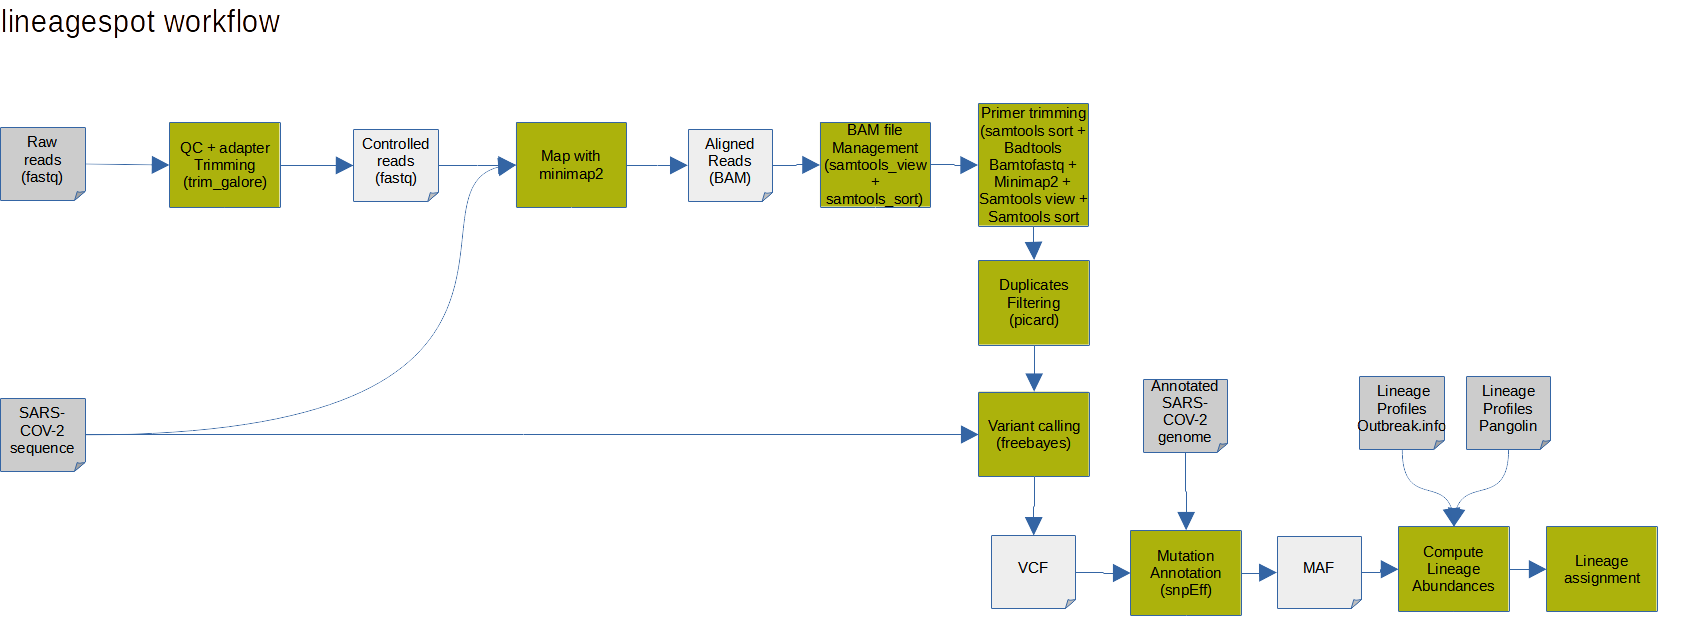
\includegraphics[width=1.4\textwidth]{figures/prior/lineagespot.png}
            \captionof{figure}{Lineagespot workflow.}
            \label{fig:prior:ls}
        \end{figure}
        \end{center}
        \vfill
        \end{landscape}
        
        \paragraph{PiGx}
        The other pipeline, PiGx SARS-CoV-2 \cite{schumann2021}, first, performs extensive quality control on the raw reads and information about primers and adapters used. Fastp \cite{chen2018} is used for adapter trimming and filtering, while iVAR is used for primer trimming. Using BWA \cite{li2013}, the trimmed reads are aligned to the reference genome of SARS-CoV-2, resulting in SAM/BAM files with aligned and unaligned reads. After alignment, MultiQC \cite{multiqc} is used to aggregate reports that check the quality of raw and processed reads. Further, PiGx checks samples for genome coverage and how many of the provided signature mutation sites, sites with mutations that characterize variants of concern or variants of interest, are covered by the sample. Every sample is given a quality score based on this. Those samples with genome coverage of less than 90\% are discarded from time series analyses and summaries.

        With LoFreq \cite{lofreq}, variants are called, and \acrshort{snvs} are inferred from aligned reads. The mutations are annotated with \acrshort{vep} \cite{mclaren2016}. 
        
        PiGx is capable of deconvoluting the frequencies of variants of concern from pooled sequencing reads. Briefly, the deconvolution method uses signature mutations for each variant of concern and tries to discern the proportions of these variants making up the observed mutation frequencies in the pooled sequencing reads obtained from the wastewater. To infer the proportions of each lineage on each sample, the deconvolution method is applied (based on the frequencies of the signature mutations). On the basis of the observed frequencies of signature mutations for each lineage, the lineage frequencies are predicted using a regression model. 
        
        After lineage frequencies prediction, PiGx generates a per-sample report that describes variants of concern and frequency of lineages from each wastewater sample. Additionally, the unaligned reads will be taxonomically classified with Kraken2 \cite{wood2014,wood2019,lu2020} to determine the abundance of RNA that matches other existing species found in unaligned reads in the wastewater samples. The diagram of PiGx pipeline is shown in \cref{fig:prior:pigx}.
        
        One of the significant benefits of PiGx method is the addition of different weights of tracked lineages based on how many signature mutations were found for each of them for a given sample. The purpose of this step is to determine which lineages have a low abundance and have only a few or only shared mutations in order to obtain more precise predictions. 

        PiGx has another advantage - controlling taxonomic classification for other species present in samples but not mapped to the SARS-CoV-2 reference sequence. With Kraken2 usage, this simple step opens opportunities for learning about sample diversity. Due to Kraken2's k-mer classification, it can also identify reads that match SARS-CoV-2 but are not aligned with stringent alignment tools. In addition, it provides insights into the possibility of losing new mutations that weren't captured in the alignment. The user can analyze potential issues here and adjust the alignment stringency if necessary.
        \begin{landscape}
        \centering\vspace*{\fill}
        \begin{figure}[H]
        	\centering
            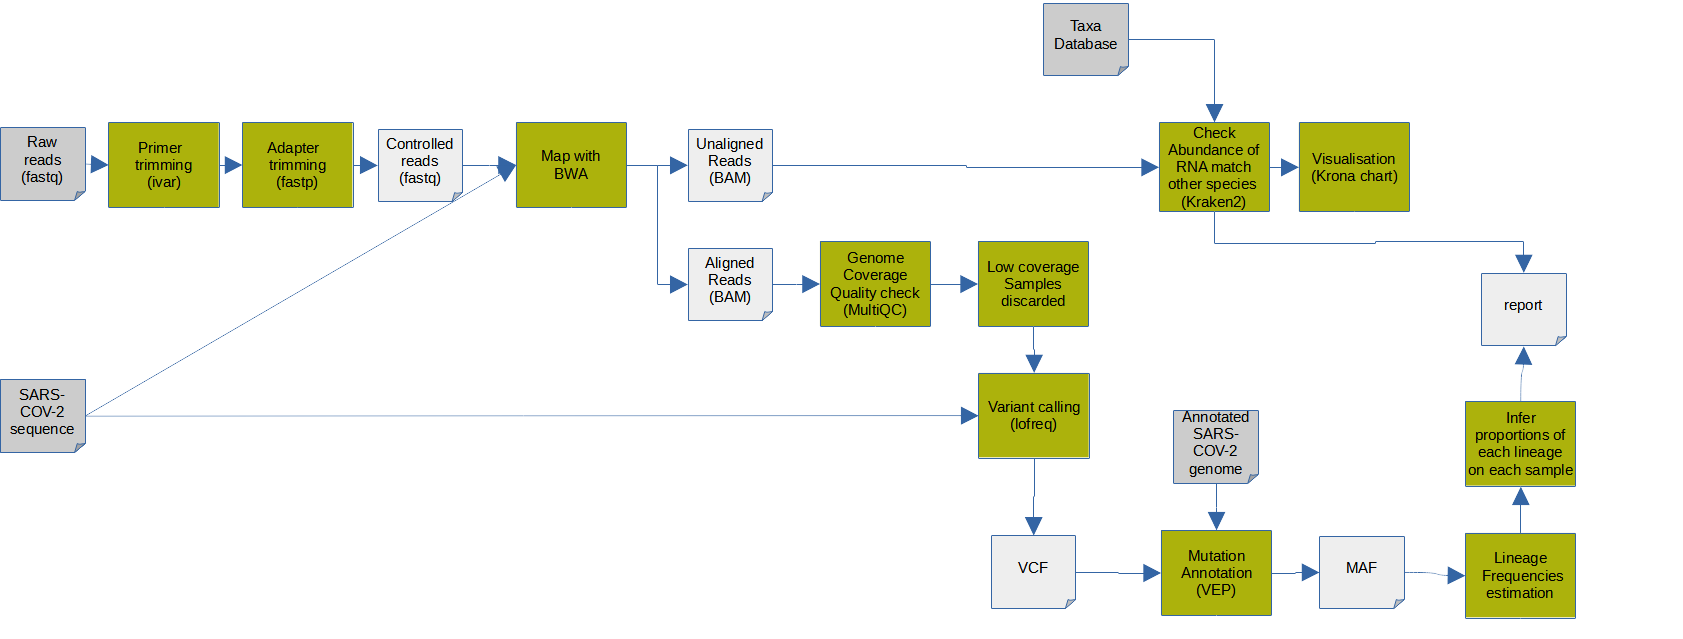
\includegraphics[width=1.5\textwidth]{figures/prior/pigx.png}
            \captionof{figure}{PiGx workflow. }
            \label{fig:prior:pigx}
        \end{figure}
        \vfill
        \end{landscape}

        \paragraph{Cowwid}
        In its turn, another approach, Cowwid \cite{jahn2021} pipeline uses steps: i) processing raw reads with the help of V-pipe \cite{posada2021} sub-workflow (performing quality controls and read filtering with FastQC and PRINSEQ \cite{babraham,prinseq}, assembly with VICUNA \cite{vicuna2012}, read alignment with BWA-MEM and ngshmmalign \cite{li2013,ngshmmalign2021} and variant calling with ShoRAH \cite{shorah}); ii) co-occurrence analysis (detecting mutation co-occurrence) with the help of COJAC \cite{jahn2022,cojac2022}; iii) building of the list of signature mutations for the variants of concern, variant mutation table, and visualization including heatmaps and curves plots generation with the help of Jupyter; iv) generation of Python script for upload to CoV-Spectrum. The diagram that describes the Cowwid workflow is presented in \cref{fig:prior:cowwid}.
        
        The advantage of Cowwid pipeline is its capability to detect lineages that are unknown as it uses COJAC tool as a co-occurance step. The other bright side of Cowwid is that its output was already experienced to be uploaded to CoV-Spectrum which means the accessibility of results and a variety of visualizations. Though, the Jupyter-based plots as well as the upload script look hard-coding, which is disadvantageous. That means that this pipeline is advanced but requires to be adjusted and generalized in order to use it for other than datasets described by K. Jahn et al. \cite{jahn2022}. 
        \begin{landscape}
        \centering\vspace*{\fill}
        \begin{figure}[ht!]
        	\centering
            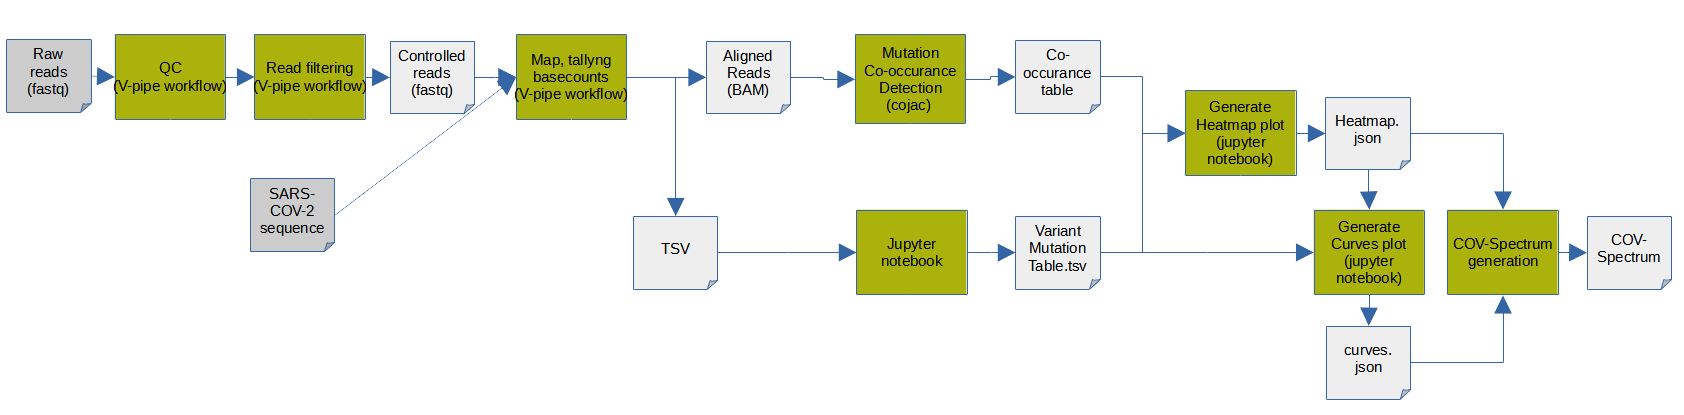
\includegraphics[width=1.4\textwidth]{figures/prior/cowwid.png}
            \captionof{figure}{Cowwid workflow.}
            \label{fig:prior:cowwid}
        \end{figure}
        \vfill
        \end{landscape}
        
        
        \paragraph{Pipeline described by R. Izquierdo-Lara et al.}
        
        Meanwhile, R. Izquierdo-Lara et al. \cite{izquierdo} used 2 different workflows using two different workflow managers (Snakemake and Galaxy). For the Nanopore data, they used Snakemake to: i) demultiplex \acrshort{fastq} raw reads using Porechop \cite{wick2022}; ii) trim of primers using Cutadapt \cite{martin2011}; iii) perform a reference-based alignment against SARS-CoV-2 reference sequence using minimap2; iv) confirm mutations in the genome by manually checking the alignment in UGENE \cite{okonechnikov2012} and resolve homopolymeric regions by consulting reference genomes. On the other hand, for the Illumina Sequence Analysis, they used Galaxy to: i) filter raw sequencing reads using Fastp \cite{chen2018}; ii) using BWA-MEM, remove adapter contamination, ambiguous bases, low quality reads (Phred score <30), and fragments <50 nt; then, map reads against GISAID sequence EPI\_ISL\_412973; iii) realign reads using FreeBayes \cite{garrison2012}; iv) generate consensus sequences and variants using iVar \cite{grubaugh2019}; v) finally, confirm variant calling by manual inspection of the aligned reads using UGENE.

        For the phylogenetic analysis, sequences were aligned with >75\% genome coverage using MAFFT \cite{mafft}, followed by visualization of trees with Figtree \cite{figtree}, and clades assignment with Nextclade tool \cite{nextclade2022}. The diagram that describes the workflow is presented in \cref{fig:prior:izquierdo}.
        
        A feature that this pipeline offers that others listed above in this section do not is phylogenetic analysis and visualization of the phylogenetic tree.
        \begin{landscape}
        \centering\vspace*{\fill}
        \begin{figure}[ht!]
        	\centering
            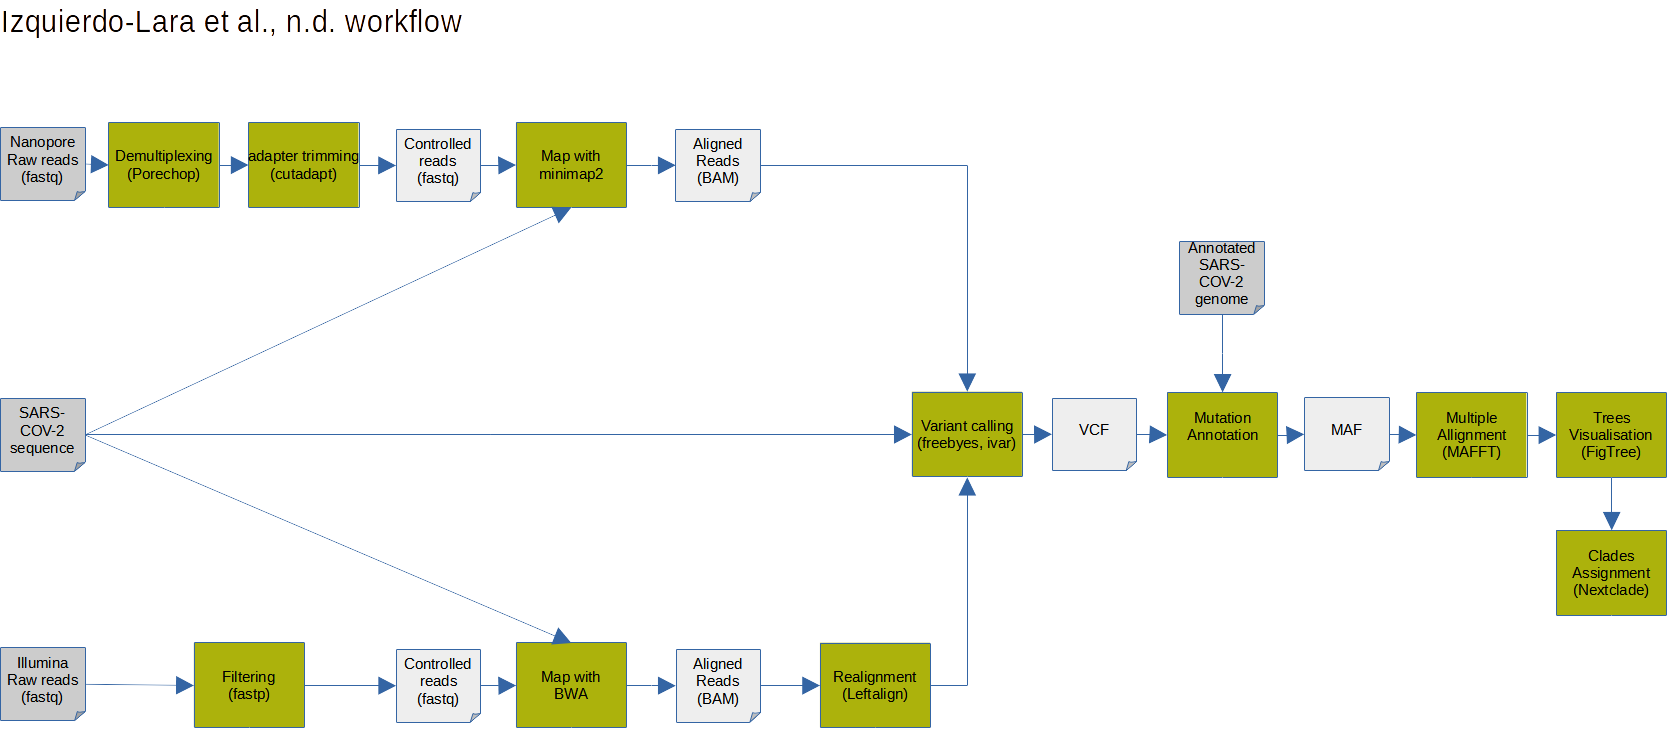
\includegraphics[width=1.4\textwidth]{figures/prior/Izquierdo-Lara.png}
            \captionof{figure}{Workflow described by R. Izquierdo-Lara et al.}
            \label{fig:prior:izquierdo}
        \end{figure}
        \vfill
        \end{landscape}
        
        
        \subsubsection{Comparison of methods for wastewater surveillance} \label{sec:prior:methods:comparison}
        To compare the existing tools and pipelines representing different state-of-the-art approaches, \cref{tab:prior:methods-tools} for individual tools and \cref{tab:prior:methods-pipelines} for standalone pipelines show some of them accompanied by source code link, license type, external tools used, description of inputs, produced outputs, their availability in Bioconda, availability in Galaxy before starting this thesis, and, finally, their prior usage (applications).
        \begin{landscape}
            \centering\vspace*{\fill}
                \begin{table}[ht!]
                \tiny
                \begin{tabular}{l|l|l|l|l|l|l|l|l|l|l}
\multicolumn{1}{m{1cm}|}{\textbf{Name}}&\multicolumn{1}{m{0.7cm}|}{\textbf{latest version}}&\multicolumn{1}{m{0.7cm}|}{\textbf{Source code}}&\multicolumn{1}{m{0.75cm}|}{\textbf{License}}&\multicolumn{1}{m{3cm}|}{\textbf{Goal}}&\multicolumn{1}{m{3cm}|}{\textbf{External tools plugged}}&\multicolumn{1}{m{3cm}|}{\textbf{Input}}&\multicolumn{1}{m{3cm}|}{\textbf{Output}}&\multicolumn{1}{m{1cm}|}{\textbf{Available in Bioconda}}&\multicolumn{1}{m{1cm}|}{\textbf{Available in Galaxy}}&\multicolumn{1}{m{1cm}}{\textbf{Applica- tions}}\\ \hline 
\multicolumn{1}{m{1cm}|}{\textbf{Freyja}}&\multicolumn{1}{m{0.7cm}|}{1.3.11}&\multicolumn{1}{m{0.7cm}|}{\cite{joshuailevy2022}}&\multicolumn{1}{m{0.75cm}|}{BSD-2-Clause (open source)}&\multicolumn{1}{m{3cm}|}{Recover relative lineage abundances from mixed SARS-CoV-2 samples from a sequencing dataset (BAM aligned to the Hu-1 reference)}&\multicolumn{1}{m{3cm}|}{-}&\multicolumn{1}{m{3cm}|}{Variant call and sequencing depth information}&\multicolumn{1}{m{3cm}|}{TSV file that includes the lineages present, their corresponding abundances, and summarization by constellation}&\multicolumn{1}{m{1cm}|}{+}&\multicolumn{1}{m{1cm}|}{-}&\multicolumn{1}{m{1cm}}{\cite{karthikeyan2022,solismoreira2022,nutrition2022,karthikeyan2022b}}\\ \hline 
\multicolumn{1}{m{1cm}|}{\textbf{COJAC}}&\multicolumn{1}{m{0.7cm}|}{0.2}&\multicolumn{1}{m{0.7cm}|}{\cite{cojac2022}}&\multicolumn{1}{m{0.75cm}|}{GPL-3.0 (open source)}&\multicolumn{1}{m{3cm}|}{Analyzing co-occurrence of mutations on amplicons}&\multicolumn{1}{m{3cm}|}{-}&\multicolumn{1}{m{3cm}|}{BAM/CRAM/SAM and BED file describing the amplified regions}&\multicolumn{1}{m{3cm}|}{Total count of amplicons carrying the sites of interest, amplicons carrying mutations on all site of interest, amplicons where one mutation is missing, fraction (ratio of number of all amplicons carrying mutations on all sites of interest to total number of amplicons carrying cites of interest) }&\multicolumn{1}{m{1cm}|}{+}&\multicolumn{1}{m{1cm}|}{-}&\multicolumn{1}{m{1cm}}{\cite{jahn2022,karthikeyan2022b,jbc}}\\ \hline 
\multicolumn{1}{m{1cm}|}{\textbf{LCS}}&\multicolumn{1}{m{0.7cm}|}{1.2.0}&\multicolumn{1}{m{0.7cm}|}{\cite{valieris2022}}&\multicolumn{1}{m{0.75cm}|}{-}&\multicolumn{1}{m{3cm}|}{Lineage decomposition for SARS-CoV-2 pooled samples}&\multicolumn{1}{m{3cm}|}{-}&\multicolumn{1}{m{3cm}|}{Variant-groups definitions, raw-fastq files pooled samples, fasta file of the primers used}&\multicolumn{1}{m{3cm}|}{Lineage decomposition outputs for SARS-CoV-2 pooled samples, plots}&\multicolumn{1}{m{1cm}|}{-}&\multicolumn{1}{m{1cm}|}{-}&\multicolumn{1}{m{1cm}}{\cite{valieris2022,karthikeyan2022b}}\\ \hline 
\multicolumn{1}{m{1cm}|}{\textbf{Kallisto}}&\multicolumn{1}{m{0.7cm}|}{0.48.0}&\multicolumn{1}{m{0.7cm}|}{\cite{bray2016}}&\multicolumn{1}{m{0.75cm}|}{BSD-2-Clause (open source)}&\multicolumn{1}{m{3cm}|}{Quantifying abundances of transcripts from RNA-Seq data, or more generally of target sequences using high-throughput sequencing reads}&\multicolumn{1}{m{3cm}|}{-}&\multicolumn{1}{m{3cm}|}{FASTQ (single-end or paired-end reads)}&\multicolumn{1}{m{3cm}|}{Abundance estimates, bootstrap estimates, and transcript length information length}&\multicolumn{1}{m{1cm}|}{+}&\multicolumn{1}{m{1cm}|}{+}&\multicolumn{1}{m{1cm}}{\cite{baaijens2021,anton2022}}\\ \hline 
\multicolumn{1}{m{1cm}|}{\textbf{Alcov}}&\multicolumn{1}{m{0.7cm}|}{-}&\multicolumn{1}{m{0.7cm}|}{\cite{ellmen2021}}&\multicolumn{1}{m{0.75cm}|}{-}&\multicolumn{1}{m{3cm}|}{Abundance learning for SARS-CoV-2 variants.}&\multicolumn{1}{m{3cm}|}{-}&\multicolumn{1}{m{3cm}|}{BAM file of reads aligned to the SARS-CoV-2 reference genome}&\multicolumn{1}{m{3cm}|}{Number of reads with and without each mutation in each sample, heatmap showing the frequencies for all samples, mutations, read depth for each amplicon, plots of amplicon GC content against amplicon depth}&\multicolumn{1}{m{1cm}|}{-}&\multicolumn{1}{m{1cm}|}{-}&\multicolumn{1}{m{1cm}}{\cite{ellmen2021}}\\ \hline 
\multicolumn{1}{m{1cm}|}{\textbf{SAM refiner}}&\multicolumn{1}{m{0.7cm}|}{1.4.0}&\multicolumn{1}{m{0.7cm}|}{\cite{gregory2021}}&\multicolumn{1}{m{0.75cm}|}{GPL-3.0 (open source)}&\multicolumn{1}{m{3cm}|}{Gathering variant information from a SAM formatted files}&\multicolumn{1}{m{3cm}|}{-}&\multicolumn{1}{m{3cm}|}{SAM formatted files generated from sequencing mapping programs such as Bowtie2 or MiniMap2, FASTA formatted file for a reference sequence}&\multicolumn{1}{m{3cm}|}{Unique sequences, statistics about removed chimera, covariant deconvolution output}&\multicolumn{1}{m{1cm}|}{+}&\multicolumn{1}{m{1cm}|}{-}&\multicolumn{1}{m{1cm}}{\cite{gregory2021,gregory2022,yaglom2022}}\\ \hline 
\end{tabular}
                \caption{Comparison table of existing individual tools for wastewater surveillance} \label{tab:prior:methods-tools}
                \end{table}

\begin{table}[ht!]
                \tiny
                \begin{tabular}{l|l|l|l|l|l|l|l|l|l|l}
\multicolumn{1}{m{1cm}|}{\textbf{Name}}&\multicolumn{1}{m{0.7cm}|}{\textbf{latest version}}&\multicolumn{1}{m{0.7cm}|}{\textbf{Source code}}&\multicolumn{1}{m{0.75cm}|}{\textbf{License}}&\multicolumn{1}{m{3cm}|}{\textbf{Goal}}&\multicolumn{1}{m{3cm}|}{\textbf{External tools plugged}}&\multicolumn{1}{m{3cm}|}{\textbf{Input}}&\multicolumn{1}{m{3cm}|}{\textbf{Output}}&\multicolumn{1}{m{1cm}|}{\textbf{Available in Bioconda}}&\multicolumn{1}{m{1cm}|}{\textbf{Available in Galaxy}}&\multicolumn{1}{m{1cm}}{\textbf{Applica- tions}}\\ \hline 
\multicolumn{1}{m{1cm}|}{\textbf{Pipes et al.}}&\multicolumn{1}{m{0.7cm}|}{1.0}&\multicolumn{1}{m{0.7cm}|}{\cite{pipes2022}}&\multicolumn{1}{m{0.75cm}|}{GPL-3.0 (open source)}&\multicolumn{1}{m{3cm}|}{Estimating the relative proportions of SARS-CoV-2 strains from wastewater samples}&\multicolumn{1}{m{3cm}|}{Bowtie2 v2.4.5}&\multicolumn{1}{m{3cm}|}{FASTA file; \acrshort{msa} FASTA of SARS-CoV-2 reference strains}&\multicolumn{1}{m{3cm}|}{Estimated proportion of candidate strains, barplot with only those strains with an estimated proportion larger than 1\%}&\multicolumn{1}{m{1cm}|}{-}&\multicolumn{1}{m{1cm}|}{-}&\multicolumn{1}{m{1cm}}{\cite{pipes2022}}\\ \hline 
\multicolumn{1}{m{1cm}|}{\textbf{Grom- stole}}&\multicolumn{1}{m{0.7cm}|}{1.0}&\multicolumn{1}{m{0.7cm}|}{\cite{gromstole2022}}&\multicolumn{1}{m{0.75cm}|}{MIT (open source)}&\multicolumn{1}{m{3cm}|}{To estimate the relative frequencies of different SARS-CoV-2 lineages}&\multicolumn{1}{m{3cm}|}{Minimap2 v2.24, Cutadapt v4.0}&\multicolumn{1}{m{3cm}|}{Paired-end reads in separate FASTQ/FASTA files, NC043312.fa as a reference genome}&\multicolumn{1}{m{3cm}|}{Counts of each mutation of the lineages, coverage at every position on the reference genome, estimate of the proportion (including 95\% confidence interval); }&\multicolumn{1}{m{1cm}|}{-}&\multicolumn{1}{m{1cm}|}{-}&\multicolumn{1}{m{1cm}}{\cite{gromstole2022}}\\ \hline 
\multicolumn{1}{m{1cm}|}{\textbf{AG}}&\multicolumn{1}{m{0.7cm}|}{-}&\multicolumn{1}{m{0.7cm}|}{\cite{nguessan2022}}&\multicolumn{1}{m{0.75cm}|}{GPL-3.0 (open source)}&\multicolumn{1}{m{3cm}|}{Analyzing the within-sample genetic diversity of SARS-CoV-2 in Wastewater samples.}&\multicolumn{1}{m{3cm}|}{Trim Galore v0.6.7, Minimap2 v2.24, SAMtools v2.0.4, iVar v1.3.1, BEDTools v2.27, Picard v2.18, FreeBayes v1.1.0.46, SnpEff v4.3}&\multicolumn{1}{m{3cm}|}{Paired-end .fastq files for each sample}&\multicolumn{1}{m{3cm}|}{Tabular files with scanned variants, common depth report}&\multicolumn{1}{m{1cm}|}{-}&\multicolumn{1}{m{1cm}|}{-}&\multicolumn{1}{m{1cm}}{\cite{nguessan2022}}\\ \hline 
\multicolumn{1}{m{1cm}|}{\textbf{Lineage- spot}}&\multicolumn{1}{m{0.7cm}|}{-}&\multicolumn{1}{m{0.7cm}|}{\cite{pechlivanis2022}}&\multicolumn{1}{m{0.75cm}|}{MIT (open source)}&\multicolumn{1}{m{3cm}|}{Identify SARS-CoV-2 related mutations based on a single (or a list) of variant(s) file(s) (i.e., variant calling format).}&\multicolumn{1}{m{3cm}|}{Trim Galore v0.6.7, FastQC v0.73, Minimap2 v2.24, SAMtools v2, BEDTools v2, Picard v2.18, FreeBayes v1.1, SnpEff v4.3}&\multicolumn{1}{m{3cm}|}{Raw fastq FASTQ files, anf for further analysis - VCF and file containing all lineage-assignment rules, as retrieved from the pangolin tool repository}&\multicolumn{1}{m{3cm}|}{VCF, MAF files, eport about lineage abundances}&\multicolumn{1}{m{1cm}|}{-}&\multicolumn{1}{m{1cm}|}{-}&\multicolumn{1}{m{1cm}}{\cite{pechlivanis2022}}\\ \hline 
\multicolumn{1}{m{1cm}|}{\textbf{PiGx}}&\multicolumn{1}{m{0.7cm}|}{0.0.8}&\multicolumn{1}{m{0.7cm}|}{\cite{schumann2021}}&\multicolumn{1}{m{0.75cm}|}{GPL-3.0 (open source)}&\multicolumn{1}{m{3cm}|}{Analyzing data from sequenced wastewater samples and identifying given lineages of SARS-CoV-2}&\multicolumn{1}{m{3cm}|}{iVar v1.3.1, Fastp v0.23.2, BWA v0.7.17.2, MultiQC v1.11, LoFreq v2.1.5, VEP , Kraken2 v2.1.1, Krona v2.7.1}&\multicolumn{1}{m{3cm}|}{Raw reads and the additional information about used primers and adapters}&\multicolumn{1}{m{3cm}|}{VCF, visualization of the development of virus over time, variants report, taxonomic classification}&\multicolumn{1}{m{1cm}|}{-}&\multicolumn{1}{m{1cm}|}{-}&\multicolumn{1}{m{1cm}}{\cite{schumann2021}}\\ \hline 
\multicolumn{1}{m{1cm}|}{\textbf{Cowwid}}&\multicolumn{1}{m{0.7cm}|}{0.7.1}&\multicolumn{1}{m{0.7cm}|}{\cite{jahn2021}}&\multicolumn{1}{m{0.75cm}|}{-}&\multicolumn{1}{m{3cm}|}{Surveillance of SARS-CoV-2 genomic variants in wastewater}&\multicolumn{1}{m{3cm}|}{V-pipe v2.99.2, FastQC v0.73, PRINSEQ v0.20.4, VICUNA, BWA-MEM v0.7.17, ShoRAH, COJAC v0.2}&\multicolumn{1}{m{3cm}|}{TSV table of the samples, YAML with definition of the variants, BED with amplicon positions for ARTIC, BED with amplicon description}&\multicolumn{1}{m{3cm}|}{YAML/CSV files with coocurrences, variant mutations table, plts to integrate to CoV-Spectrum}&\multicolumn{1}{m{1cm}|}{-}&\multicolumn{1}{m{1cm}|}{-}&\multicolumn{1}{m{1cm}}{\cite{jahn2021,swisscovspectrum}}\\ \hline 
\multicolumn{1}{m{1cm}|}{\textbf{Izquierdo -Lara et al.}}&\multicolumn{1}{m{0.7cm}|}{-}&\multicolumn{1}{m{0.7cm}|}{\cite{izquierdo}}&\multicolumn{1}{m{0.75cm}|}{-}&\multicolumn{1}{m{3cm}|}{Monitoring SARS-CoV-2 Circulation and Diversity through Community Wastewater Sequencing, the Netherlands and Belgium}&\multicolumn{1}{m{3cm}|}{Porechop v0.2.4, Cutadapt v4.0, UGENE, Fastp v0.23.2, BWA-MEM v0.7.17, FreeBayes v1.1, iVar v1.3.1}&\multicolumn{1}{m{3cm}|}{Raw reads and the additional information about used primers and adapters}&\multicolumn{1}{m{3cm}|}{VCF, MAF files, Trees visualization (Fig tree)}&\multicolumn{1}{m{1cm}|}{-}&\multicolumn{1}{m{1cm}|}{-}&\multicolumn{1}{m{1cm}}{\cite{izquierdo}}\\ \hline 
                \end{tabular}
                \caption{Comparison table of existing standalone pipelines for wastewater surveillance} \label{tab:prior:methods-pipelines}
                \end{table}
                \vfill
            \end{landscape}
        

    \subsection{Discussion of existing methods} \label{sec:prior:discussion}
    A number of methods were described above that use different models to determine SARS-CoV-2 lineages and their abundances in wastewater samples. Several of the methods listed can be applied to the purpose of this thesis, i.e., improvement of existing Galaxy workflows for analyzing SARS-CoV-2 clinical samples, repurposing them to detection of SARS-CoV-2 variants in wastewater samples as well as discerning of lineage abundances in these samples. It should be pointed out that, in \cref{sec:prior:methods:tools}, separate tools are listed that focus directly on lineage abundance computation, whereas, in \cref{sec:prior:methods:pipelines}, complete and almost complete standalone pipelines like PiGx, Lineagespot, Cowwid, etc. are listed that include the entire raw reads bioinformatics analysis. Standalone pipelines are not intended to be improved in this work because they cannot be incorporated into existing Galaxy workflows for SARS-CoV-2 surveillance since Galaxy workflows offer their own independent data preprocessing. Conversely, individual tools that are capable of being plugged into currently available Galaxy workflows and performing lineage abundances computation are the interest of this thesis.

    Two tools, Freyja \cite{joshuailevy2022,karthikeyan2022} and COJAC \cite{jahn2021}, were a choice to use in the workflows to achieve the goal of this thesis because their use in various projects (such as wastewater monitoring of SARS-CoV-2 in the Center for Food Safety and Applied Nutrition in US \cite{nutrition2022}, wastewater monitoring of SARS-CoV-2 variants in Switzerland \cite{jahn2022} and in England \cite{jbc}) has shown decent results; and because of their ability to be integrated into existing Galaxy pipelines that use Galaxy workflow manager, which meets all crucial characteristics like transparency, accessibility, and reproducibility. Furthermore, Galaxy pipelines perform decent data preprocessing steps and have shown promising results on clinical data, making them worthy of being repurposed for wastewater data using tools such as Freyja and COJAC. 
    
    Interestingly for this thesis, these tools are different in purpose; for example, Freyja’s output is easy to interpret without some specific knowledge, while COJAC requires more knowledge to be used. First of all, it demands some knowledge in programming as the output of COJAC is quite raw so far and has to be processed for downstream analysis like plotting and integrating to remote platforms such as CoV-Spectrum. Second of all, the usage of COJAC requires some knowledge of virology. Despite this, COJAC provides more detailed information and is able to detect unknown variants. These two different tools, Freyja and COJAC, target different user groups (e.g., politicians and researchers), which is interesting for this thesis's research purposes.
    
%%%%%%%%%%%%%%%%%%%%%%%%%%%%%%%%%%%%%%%%%%
% Master Thesis 
% Polina Polunina
% October 2022 
%
% License:
% CC-BY-SA 4.0 -- Creative Commons Attribution-ShareAlike 4.0 International
% https://creativecommons.org/licenses/by-sa/4.0/legalcode
%%%%%%%%%%%%%%%%%%%%%%%%%%%%%%%%%%%%%%%%%%
\section{Methods} \label{sec:methods}
In the following sections, the technical details of the methods used within the thesis will be discussed. First, an evaluation of needs, including currently available data, will be described in \cref{sec:methods:needs}, followed by an explanation of existing Galaxy workflows in \cref{sec:methods:existing}. Then, \cref{sec:methods:changes} will discuss improvements of existing steps in these workflows and the addition of new steps. The following \cref{sec:methods:evaluation} will expose metrics for the evaluation of workflows and the characteristics of their comparison to other methods. Particularly, \cref{sec:methods:evaluation:mock} will give details of benchmarking with regard to the other state-of-the-art approach. Then, \cref{sec:methods:evaluation:real} will give an explanation of benchmarking results produced by both workflows on chosen real-world datasets.

    \subsection{Workflow reengineering} 
        \subsubsection{Evaluation of the needs} \label{sec:methods:needs}
            \paragraph{Characteristics to be considered for improvement}
            The purpose of this master thesis is to create Galaxy workflows to detect lineages and sub-lineages of SARS-CoV-2 in wastewater samples as well as the co-occurrence of different lineages in the sample. The workflow development was focused on the following questions to be able to: i) delineate lineages and sublineages; ii) delineate mixtures of at least two lineages of varying frequencies; iii) detect lineages at very low frequencies in mixtures; iv) delineate recombinants \cite{simonloriere2011}; v) detect in low coverage samples; vi) detect with short-read sequencing data; 7) detect with long-read sequencing data.
            
            \paragraph{Available data}
            For the purpose of this thesis, datasets from ENA database \cite{ena} were checked and analyzed. The ENA sequence read archive contained 13,893 raw read SARS-CoV-2 in wastewater datasets at the end of May 2022. Real-world data were obtained using library preparation techniques: i) ampliconic-based, and ii) metatranscriptomics (including Targeted-Capture \cite{critschristoph}, RNASeq, and \acrfull{wgs}); and sequenced using platforms: i) \acrshort{illumina}, ii) \acrshort{nanopore}, iii) ION-Torrent, iv) BGISEQ \cite{fang2018}, and v) DNBSEQ \cite{rao2020}.

            The main statistical numbers are presented in \cref{tab:intro:ww-realdata}. The amount of data influenced the decision for creating methods to analyze SARS-CoV-2 data with Galaxy workflows. Illumina-based Ampliconic data remain to be the most commonly obtained for wastewater samples (as it was for clinical data \cite{maier2021b}).
            
            \begin{table}[ht!]
                \centering
                \small
                \begin{tabular}{lllll}
               \textbf{Library}        & \textbf{Sequencing} &  \textbf{Library}    & \textbf{Number}   & \textbf{Number} \\ 
                \textbf{Strategy}        & \textbf{platform} & \textbf{Layout}    & \textbf{of accessions}   & \textbf{of samples} \\ \hline
                \textbf{Ampliconic:}                        &BGISEQ                      &  \acrlong{pe}                & 1              & 48 \\
                                       &  DNBSEQ                      & \acrlong{pe}                 & 1              & 59 \\
                                    & \acrshort{illumina}         & \acrlong{pe}                   & 21              & 8,293 \\
                &                 Ion Torrent                   & \acrlong{se}             & 4          & 65 \\ 
                 &                  \acrshort{nanopore}                 & \acrlong{se}             & 4          & 169\\ 
                  \textbf{Ampliconic Total}                 &             &           & \textbf{31}              & \textbf{8,634} \\   \hline 
               \textbf{Metatranscriptomics:}        &                      &           &               & \\
               RNA-Seq                             &    \acrshort{illumina}           &  \acrlong{pe}            & 1              & 173 \\
                Targeted-Capture                          &   \acrshort{illumina}                 &  \acrlong{pe}            & 1              & 11 \\
                 \acrshort{wgs}                          &    \acrshort{illumina}               &  \acrlong{pe}            & 12              & 5,146 \\
                                  &    \acrshort{nanopore}               &  \acrlong{pe}            & 3              & 122 \\
                  \textbf{Metatranscriptomics Total}                 &             &           & \textbf{17}              & \textbf{5,452} \\   \hline
                \textbf{Total}                 &  &             & \textbf{49}           & \textbf{14,086}\\ \hline
                \end{tabular}
                \caption{Overall numbers of accessions and samples of different types of data for SARS-CoV-2 in wastewater datasets in ENA. The table was created using a PivotTable in Google Sheets. Metadata about real-world datasets were uploaded from ENA to Google Sheets, then, Pivot table was generated to analyze numerical data. First, data was sorted by Library strategy, following with sorting by Sequencing platform, Labrary Layout. Next, count of accessions and sum of samples were calculated.} \label{tab:intro:ww-realdata}
            \end{table}
            
            The heatmap plot in \cref{fig:methods:data-heatmap} was created with Python using Seaborn visualization library \cite{waskom2021} based on Matplotlib \cite{hunter2007} to depict the number of wastewater samples received using different sequencing methods and library preparation strategies that are publicly available in ENA. Obviously, Illumina-based Ampliconic is the most common type of data sequencing, followed by Illumina-based with \acrshort{wgs} library preparation strategy. To address this, I developed workflows for Illumina-based data in this master's thesis, both for ampliconic and metatranscriptomic library preparation techniques.
            \begin{figure}[ht!]
            	\centering
                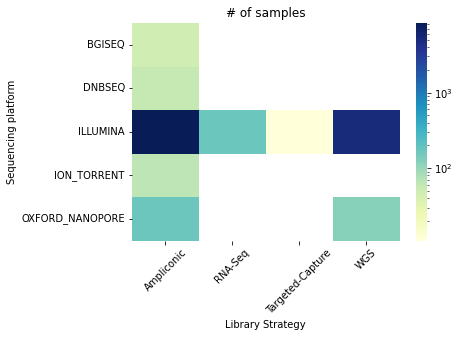
\includegraphics[width=0.7\textwidth]{figures/methods/datasets-heatmap.png}
                \captionof{figure}{Number of samples available for each sequencing platform and library preparation strategy for SARS-CoV-2 in wastewater according to ENA archive as of May 2022. BGISEQ, DNBSEQ, ILLUMINA, ION\_TORRENT, and OXFORD\_NANOPORE refer to corresponding sequencing technologies. Ampliconic library strategy refers to library preparation based on amplicons, while RNA-Seq, Targeted-Capture, and \acrshort{wgs} refer to types of metatranscriptomic-based library preparation strategy.}
                \label{fig:methods:data-heatmap}
            \end{figure}
       
        \subsubsection{Evaluation of the existing Galaxy workflows} \label{sec:methods:existing}
        Galaxy was used as a workflow manager for this thesis. The Galaxy facilitates open and accessible platforms that can ensure data analysis transparency and reproducibility. There are three global Galaxy instances where the workflow can be accessed immediately and for free. Thousands of users can run hundreds of thousands of analyses per month on each system. Using the service, the user will have access to as much computation as they need (with a limit on the number of simultaneous analyses) and 250GB of disk space, which can be increased based on usage. 

        Moreover, Galaxy provides infrastructure that already contains loads of existing tools, and tools can be added to Galaxy with the help of Planemo \cite{planemo}. It serves as a decent basis for workflow development. Additionally, Galaxy provides automated bots \cite{bots2022} for genome data surveillance which opens the opportunity to be used for SARS-CoV-2 wastewater surveillance workflows in order to analyze data regularly.
        
        The four existing workflows are taken as a basis for this thesis. Diagrams that show these workflows step by step are shown in \cref{fig:methods:artic-wf} and \cref{fig:methods:wgs-wf} for the one taken as basis in this thesis, and in \cref{fig:further:ont-wf} and \cref{fig:further:illumina-wf} in \cref{sec:appendix:figures:wfs} that were not taken as basis in this thesis. They show trustworthy results on clinical SARS-CoV-2 data and are expected to perform well on wastewater data. 
        
        Depending on available data and the prevalence of Illumina sequenced data, two out of four Galaxy existing workflows are improved: Illumina-ampliconic oriented (\cref{fig:methods:artic-wf}) and Illumina-metatranscriptomics oriented (\cref{fig:methods:wgs-wf}). 
        \begin{landscape}
        \centering\vspace*{\fill}
        \begin{figure}[ht!]
            \centering
            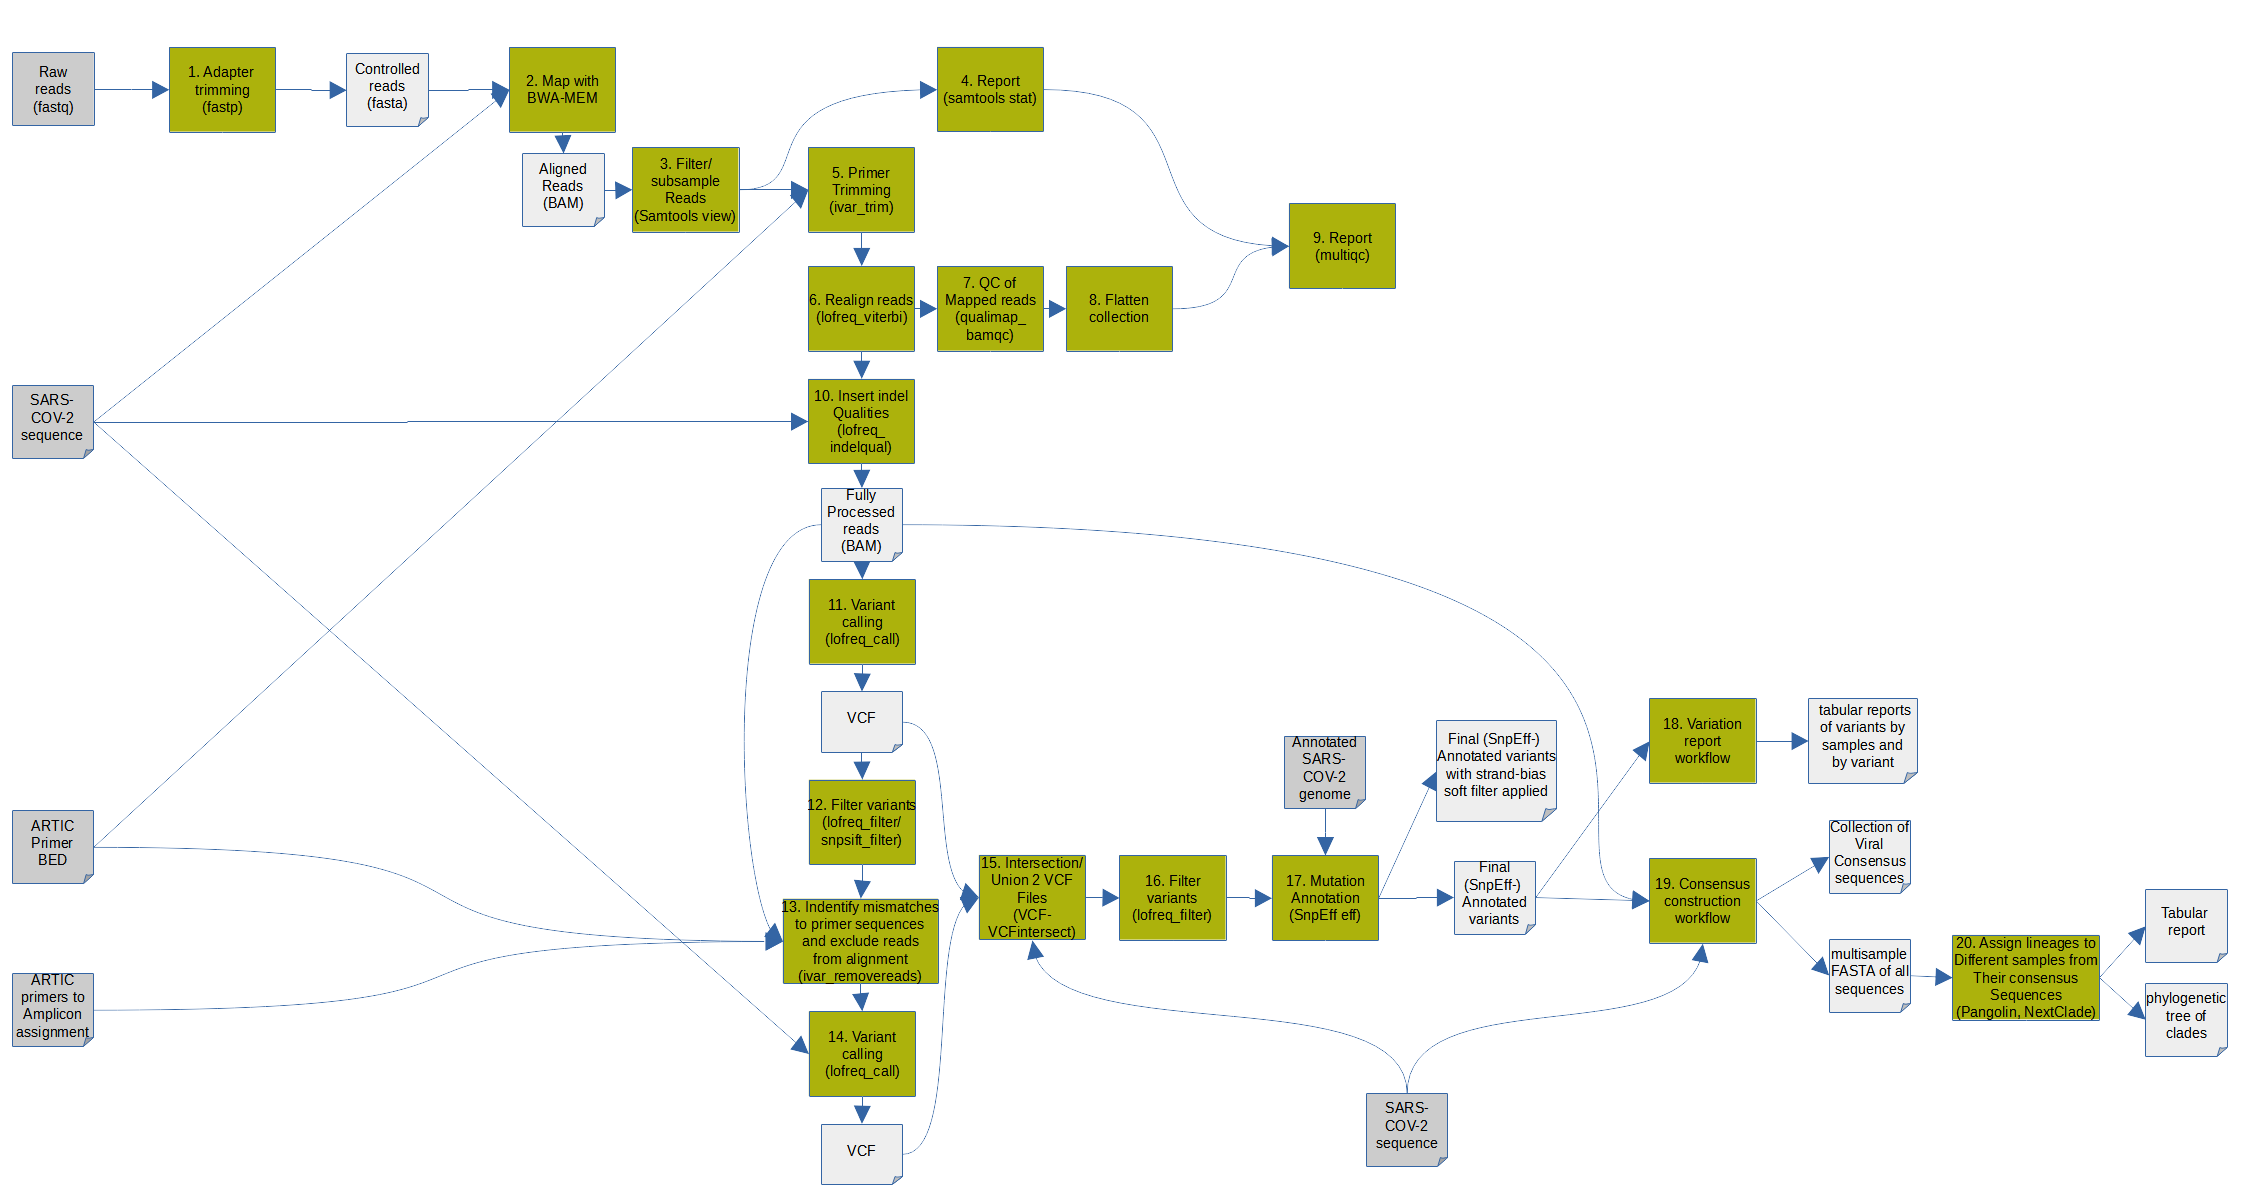
\includegraphics[width=1.4\textwidth]{figures/methods/artic-wf-before.png}
            \captionof{figure}{One of four existing Galaxy workflow for SARS-CoV-2 clinical data surveillance for paired-end reads data extracted with ampliconic-based technique and sequenced with Illumina sequencing approach.}
            \label{fig:methods:artic-wf}
        \end{figure}
        \begin{figure}[ht!]
            \centering
            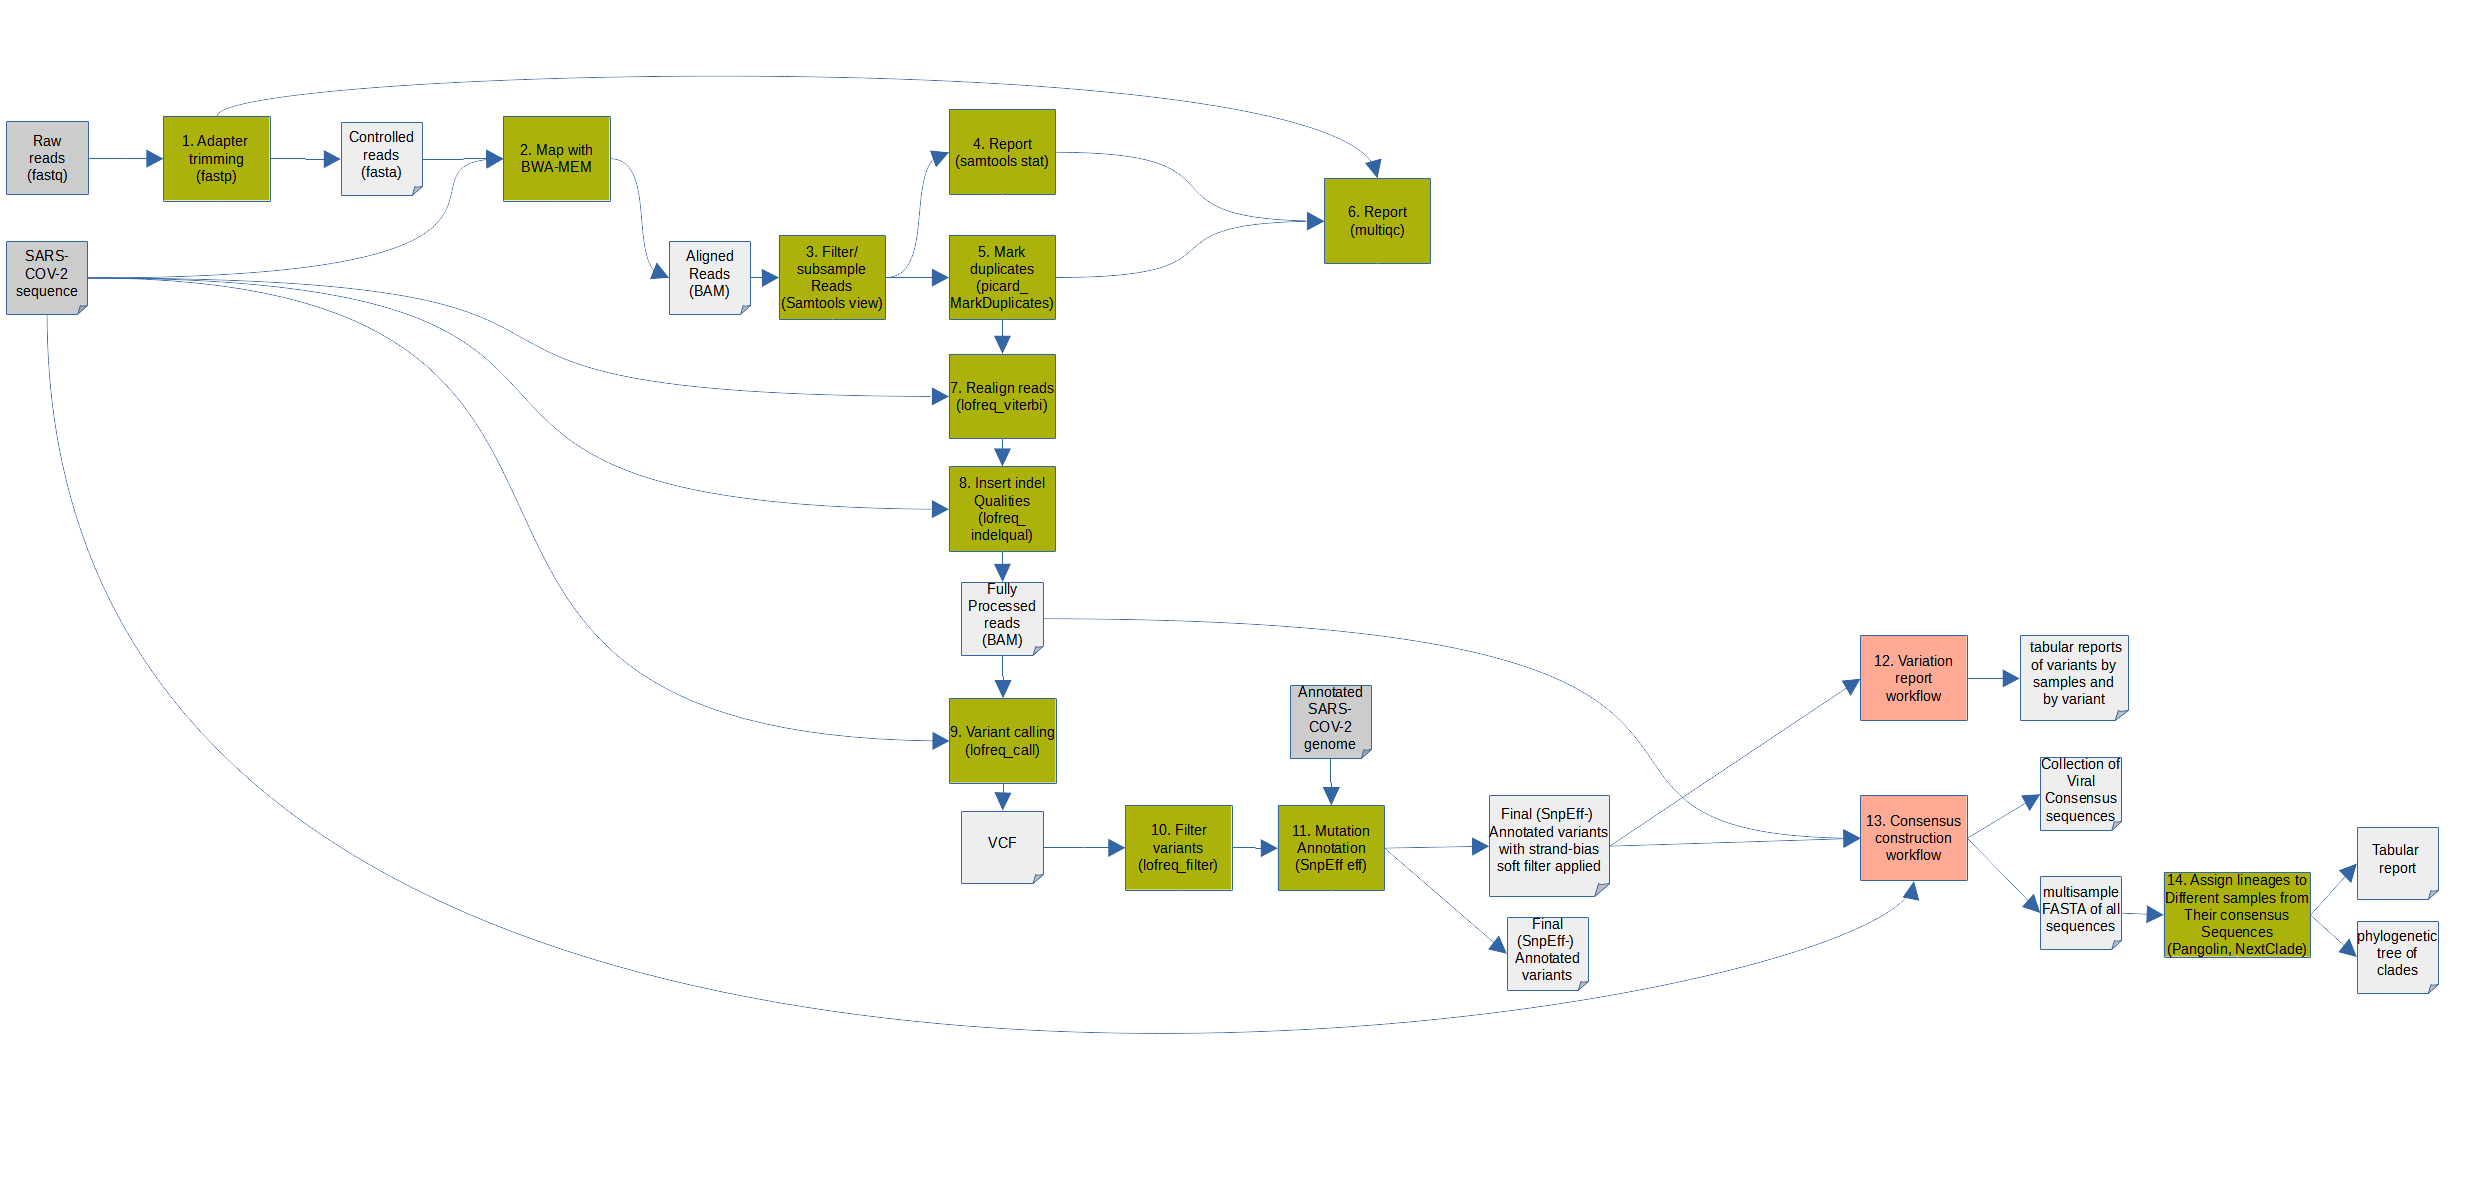
\includegraphics[width=1.4\textwidth]{figures/methods/metatranscriptomics-wf-before.png}
            \captionof{figure}{One of four existing Galaxy workflow for SARS-CoV-2 clinical data surveillance for paired-end reads data extracted with ampliconic-based technique and sequenced with Illumina sequencing approach.}
            \label{fig:methods:wgs-wf}
        \end{figure}
        \vfill
        \end{landscape}
        
        One of the main influences on the decision to take these workflows as a basis for the work in this thesis is preprocessing steps. Preprocessing steps from these workflows were used: i) quality control, ii) adapter trimming, iii) mapping to reference sequence, iv) primer trimming (for the one ampliconic-based where primers were used), v) steps that remove duplicate reads and realign them afterward with reference sequence to prepare data for vi) variant calling. In other words, the sub-workflow for preprocessing data until receiving the VCF file is taken to be: i) improved and ii) extended with the aim of delineating SARS-CoV-2 variants in wastewater samples.Tools differ for different types of datasets and depend on the library preparation approach and sequencing technique as well as on the types of reads obtained (paired-end or single-end). 
        
        In the following \cref{sec:methods:changes}, changes applied to existing Galaxy workflows will be shown, starting with expected input in \autoref{sec:methods:changes:input}, expected output in \autoref{sec:methods:changes:output}, followed by \autoref{sec:methods:changes:improvement} and \autoref{sec:methods:changes:wrappers} where new steps added will be described. Finally, \autoref{sec:methods:changes:step-by-step} will give a picture of workflows improved and repurposed for wastewater surveillance in accordance with the purpose of this thesis. 

        \subsubsection{Changes} \label{sec:methods:changes}
            \paragraph{Input data} \label{sec:methods:changes:input}
            Expected input for both ampliconic-based and metatranscriptomic-based workflows consists of i) a collection of paired-end reads samples of the considered dataset in \acrshort{fasta}/\acrshort{fastq} format; ii) \acrshort{fasta} file of reference SARS-CoV-2 sequence. Additionally, both workflows recommend providing, optionally, though: iii) UShER bar-codes file for lineage assignment used by Freyja; iv) descriptions of variants of concern in \acrshort{json} format used by COJAC. Inputs 3 and 4 are provided by a workflow as well. However, they can be outdated because the updates for both tools happen with a delay. It can happen in case of new variant appearance that up-to-date variants description files are required; hence, the opportunity of submitting them by hand directly to workflow is given.
    
            Moreover, for the workflow that is supposed to work with ampliconic-based datasets extracted using ARTIC protocol, the following input data is necessary: v) \acrshort{bed} file with ARTIC primers description; vi) description file of ARTIC primers to amplicon assignments that is ued by iVar trim and iVar removereads for assigning primers to amplicons. 

            \paragraph{Output data} \label{sec:methods:changes:output}
            In both (ampliconic-based and metatranscriptomic-based) workflows, two distinct branches are developed. The first branch focused on using Freyja tool and its outputs, while the second branch produces results based on COJAC tool usage. The user is provided to use only one of these branches as well as both of them simultaneously. Therefore, depending on the branch run in this workflow, different outputs will be obtained.
            
            The first option is based on Freyja tool for the delineation of SARS-CoV-2. Due to Freyja's use of the UShER phylogenetic tree, the output of the workflow is high-level rough reports, the proportions of specific lineages (e.g. Omicron, Delta, etc.), and their co-occurrences. Reports in this branch can be made in PDF and HTML interactive formats. Additionally, if the metadata file describing samples metadata (date of collection, viral load, etc.) is provided by a user, various plots show the dynamics of SARS-CoV-2 over time.
            
            The second branch, in turn, is based on COJAC tool for delineation. These tools provide more detailed information about variants of concern. It is possible to describe new variants in COJAC that can turn into \acrshort{vocs}. This feature makes it possible to use this tool and the COJAC-based workflow to connect with CoV-Spectrum. Even though the script for upload to CoV-Spectrum is not automated yet, it can be applied separately based on tabular output from COJAC. 

            \paragraph{Improvement of preprocessing subworkflows} \label{sec:methods:changes:improvement}
            The initial phase of workflows development in this thesis is to take subworkflows from existing workflows responsible for data preprocessing and improve them, taking into account the goal of wastewater surveillance. 

            One of the improvements made in workflows is the addition of a decontamination step. There were several reasons why a decontamination step was added to the workflow. The first and foremost reason is to eliminate any potential concerns about the anonymity of the host of the virus. Considering that SARS-CoV-2's hosts are predominantly humans and in this master thesis, I am working with wastewater which by default contains the human genome, that seemed to be a good idea to decontaminate samples from the human genome in the beginning. Additionally, this step is added to improve the runtime and accuracy of mapping from the sequence of a virus to a reference virus sequence. 
            
            Including decontamination in workflows relies on the fact that human contamination is inevitable in wastewater samples. ReadItAndKeep tool \cite{hunt2022} was added after adapter trimming (with Fastp tool) for both workflows to only keep reads matching the SARS-CoV-2 genome so that host reads could be removed from sequencing data for SARS-CoV-2. 
            
            Another step added to both workflows is a taxonomic analysis of reads that are unmapped to reference SARS-CoV-2.  I added two tools, Kraken 2 \cite{wood2014,wood2019,lu2020} and Visualization with Krona chart \cite{ondov2011,cuccuru2014}. 
            
            The tool Kraken 2 is a taxonomic sequence classifier that classifies reads according to their taxonomic labels. In order to accomplish this, it examines the k-mers within a read and queries a database with them. A taxonomic tree of all genomes that contain a given k-mer contains a mapping from Kraken's genomic library to its \acrfull{lca}. To create a taxonomic label for a read, the \acrshort{lca} taxa corresponding to its k-mers are analyzed. Labels can refer to any of the taxonomic nodes. In workflows, the viral genomes database was applied.
            
            The other tool, Krona chart, is an intuitive visualization tool that helps visualize relative abundances and confidences in multiple metagenomic classifications. Radial, space-filling displays are combined with parametric coloring and interactive zooming in polar coordinates in Krona. Using HTML5 and JavaScript, the charts can be interactively explored by any Web browser \cite{ondov2011}.
            
            It is possible to use these tools to learn about other species of bacteria that can be found in wastewater samples in addition to SARS-CoV-2. A taxonomical analysis, as well, opens the possibility of detecting newly emerged variants of SARS-CoV-2 because otherwise, they would not be able to match reference sequences and, therefore, will not be noticed. By taking this additional step, we close not only the interest in other species that wastewater samples contain and can be useful outside of SARS-CoV-2 topic but also contribute to the possibility of catching new variants of SARS-CoV-2. 
            
            One other step that should be mentioned is computing sequence depths with Samtools depth \cite{li2009}. It was added into both workflows after mapping to the reference step because the information about sequencing depths is required as input for the demixing command of Freyja tool.
            
            \paragraph{Tool integration} \label{sec:methods:changes:wrappers}
            Apart from the improvement of the existing preprocessing sub-workflow, new steps were added with the intention to reaching the goal of this thesis: to identify SARS-CoV-2 lineages in wastewater samples. In this regard, I have added delineating steps to both branches of the workflow based on Freyja and COJAC tools. These tools were chosen as individual tools that can be plugged into Galaxy workflow and represent different types of SARS-CoV-2 lineages abundances analysis and outputs that can be benchmarked afterward with each other as well as with outputs from the outside non-Galaxy standalone workflow for evaluation.

            To facilitate this master thesis, I developed Galaxy wrappers for tools that did not have one.  For that, I used Planemo \cite{planemo}, a command-line application for creating Galaxy tools, workflows, and training materials. Planemo is also used to deploy tools and workflows (tools to Galaxy ToolShed; workflows to Intergalactic Workflow Commission) as well as execute Galaxy-based analyses by command line if one prefers that interface to Galaxy's graphical interface.
            
            In designing both tools, detailed consideration was given to the user interfaces. A wrapper was designed not only to accommodate the needs of this master thesis research but also to be able to be used by researchers who are interested in using both tools independently on any Galaxy instance (e.g. \url{https://usegalaxy.eu/}, \url{https://usegalaxy.com/}, \url{https://usegalaxy.org.au/}, etc.) and also included in the specific workflow. While designing tool wrappers, enough effort was put in, in order to make the interface convenient as well as functional.
            
            For example, features like samples name autodetection and the option to provide samples names by the user, or the option to use variant descriptions of SARS-CoV-2 variants of concern cached in Galaxy as well as the option to provide the user's preferred list of variant descriptions were included. Another example is the ability to combine different types of output plots for Freyja. Additionally, for COJAC, the possibility of receiving various output tables (e.g. line-oriented, column-oriented, or multilevel-oriented) was provided. 
            
            Overall, for Freyja tool, there were four wrappers created: i) Freyja: Call variants and get sequencing depth information (\cref{list:methods:wrapper-freyja-call}), although, it was not needed for this thesis because Galaxy workflows are elaborated to call variants in a more precise way; ii) Freyja: Bootstrapping method (\cref{list:methods:wrapper-freyja-boot}), which was not used in this thesis either but was designed anyway for the perspective usage by interested users; iii) Freyja: Demix lineage abundances (\cref{list:methods:wrapper-freyja-demix}); iv) Freyja: Aggregate and visualize demixed results (\cref{list:methods:wrapper-freyja-agg}). Throughout this thesis, the last two tools were applied to both workflows. All Freyja tools are combined in the collection and maintained via macros (\cref{list:methods:wrapper-freyja-macros}).
            
            Withal, for COJAC tools, there were three wrappers designed: i) Cojac: mutbamscan scan an alignment file for mutation co-occurrences (\cref{list:methods:wrapper-cojac-mutbamcsan}), where the output is generated in \acrshort{json}, \acrshort{yaml}, and/or \acrshort{csv} table format; ii) Cojac: tabmut (\cref{list:methods:wrapper-cojac-tabmut}) export cooccurrence mutations as a table that interprets Cojac mutbamscan into nicer and readable tabular format; iii) Cojac: pubmut (\cref{list:methods:wrapper-cojac-pubmut}) render a \acrshort{json} or \acrshort{yaml} file to a pretty table that produces output in \acrshort{csv} and/or \acrshort{html} format which is pretty enough to be included in publications. All COJAC tools are combined in the collection and maintained via macros (\cref{list:methods:wrapper-cojac-macros}). Cojac: pubmut was added to Galaxy only for the case of potential interest in it outside workflows and was not directly used in the workflows developed to achieve the thesis's goal. Cojac: mutbamscan and Cojac: tabmut, in their turn, were used in the workflow corresponding to data obtained with the ampliconic library preparation method. Although COJAC can work with ampliconic data, it was not created to work with metatranscriptomic data. 
            
            Once wrappers are ready and tested, I contributed to galaxyproject/tools-iuc (available in the fork \url{https://github.com/PlushZ/tools-iuc}) to make Freyja and COJAC available to Galaxy. The tools were also added to usegalaxy.eu. 
            
            \paragraph{Workflows step by step} \label{sec:methods:changes:step-by-step}
            The final workflows developed in this master thesis are depicted in \cref{fig:methods:artic-wf-after} and \cref{fig:methods:wgs-wf-after} for Illumina ampliconic paired-end SARS-CoV-2 wastewater surveillance and for Illumina metatranscriptomic paired-end SARS-CoV-2 wastewater surveillance, respectively. In green, steps kept from existing Galaxy workflows for clinical SARS-CoV-2 data surveillance are depicted. Newly added steps for the target of this master thesis are indicated in orange. On the diagram, there is also a step called CoV-Spectrum colored pink. So far, this step is not automated and can be done only manually. Nonetheless, future improvements outside of this thesis could automate this step.
            \begin{landscape}
            \centering\vspace*{\fill}
            \begin{figure}[ht!]
                \centering
                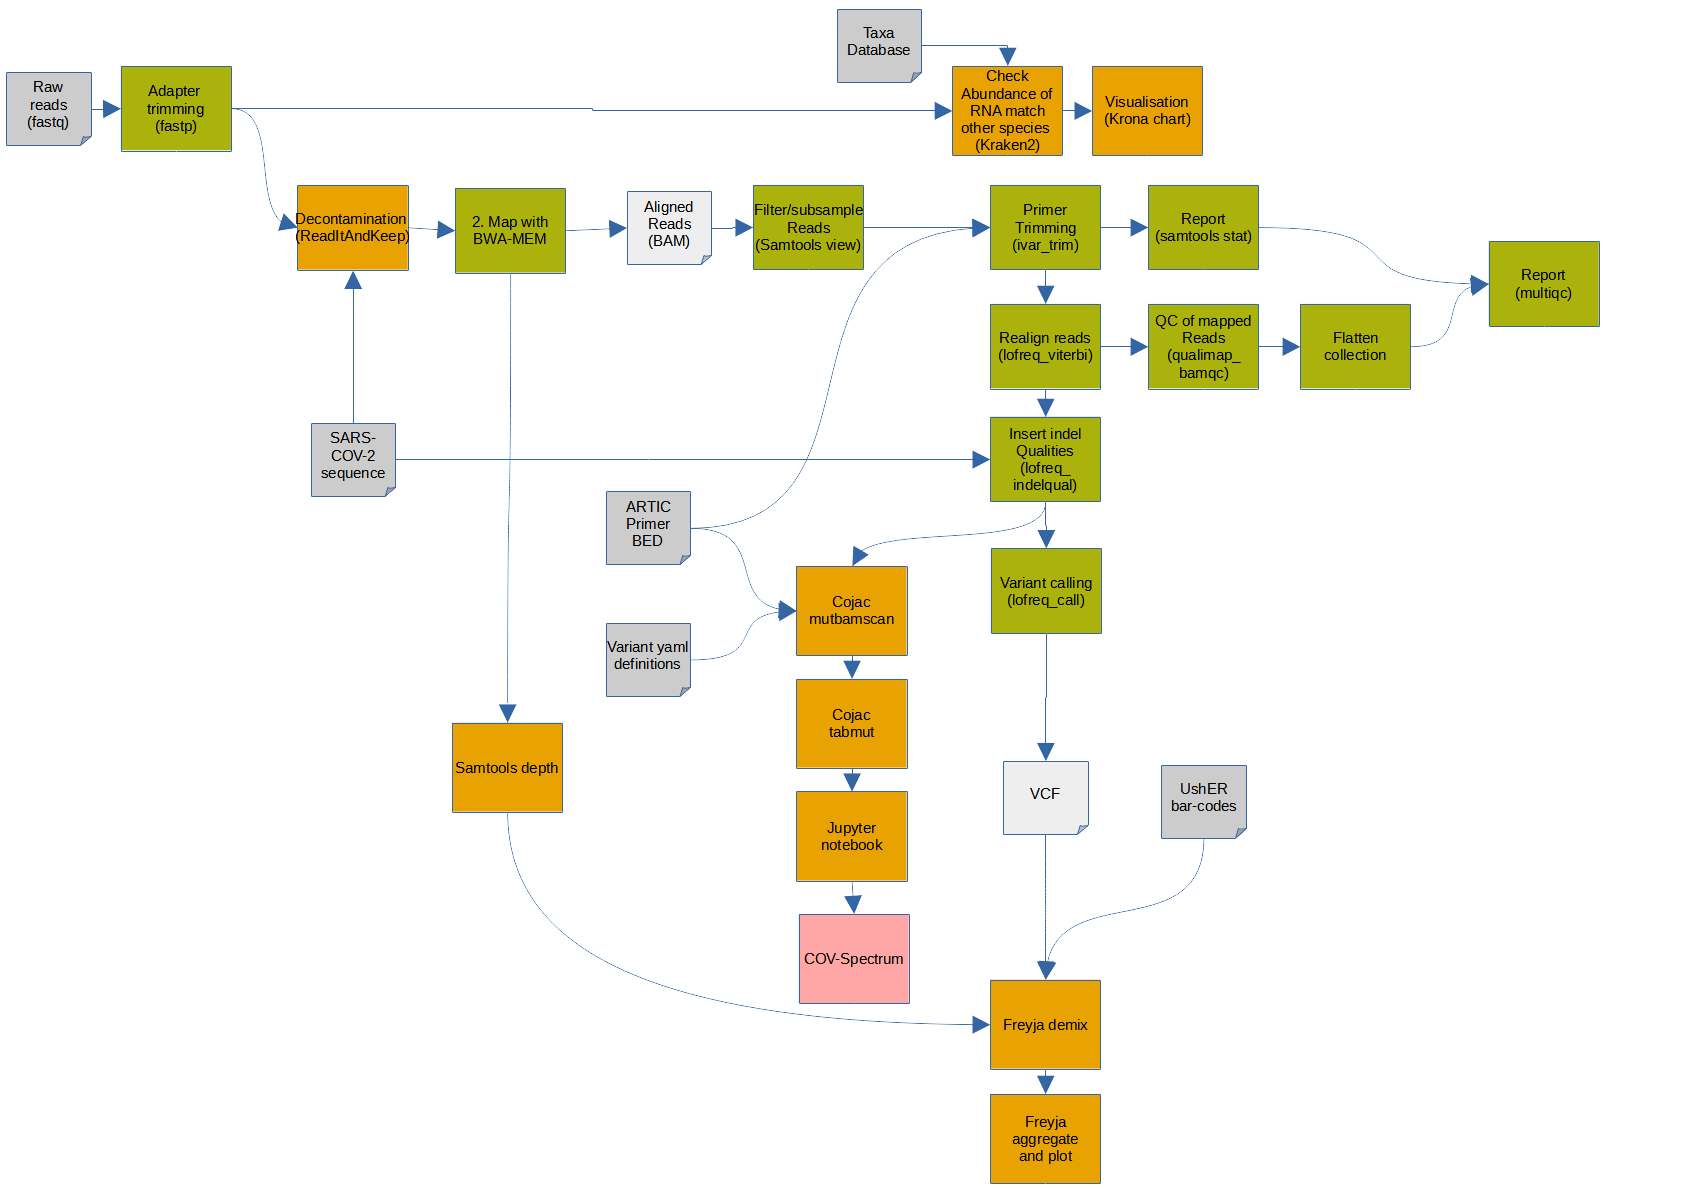
\includegraphics[width=1.2\textwidth]{figures/methods/artic-wf-after.png}
                \captionof{figure}{Improved and repurposed to SARS-CoV-2 wastewater surveillance Galaxy workflow for paired-end data extracted with ampliconic-based technique and sequenced with Illumina sequencing approach.}
                \label{fig:methods:artic-wf-after}
            \end{figure}
            \begin{figure}[ht!]
                \centering
                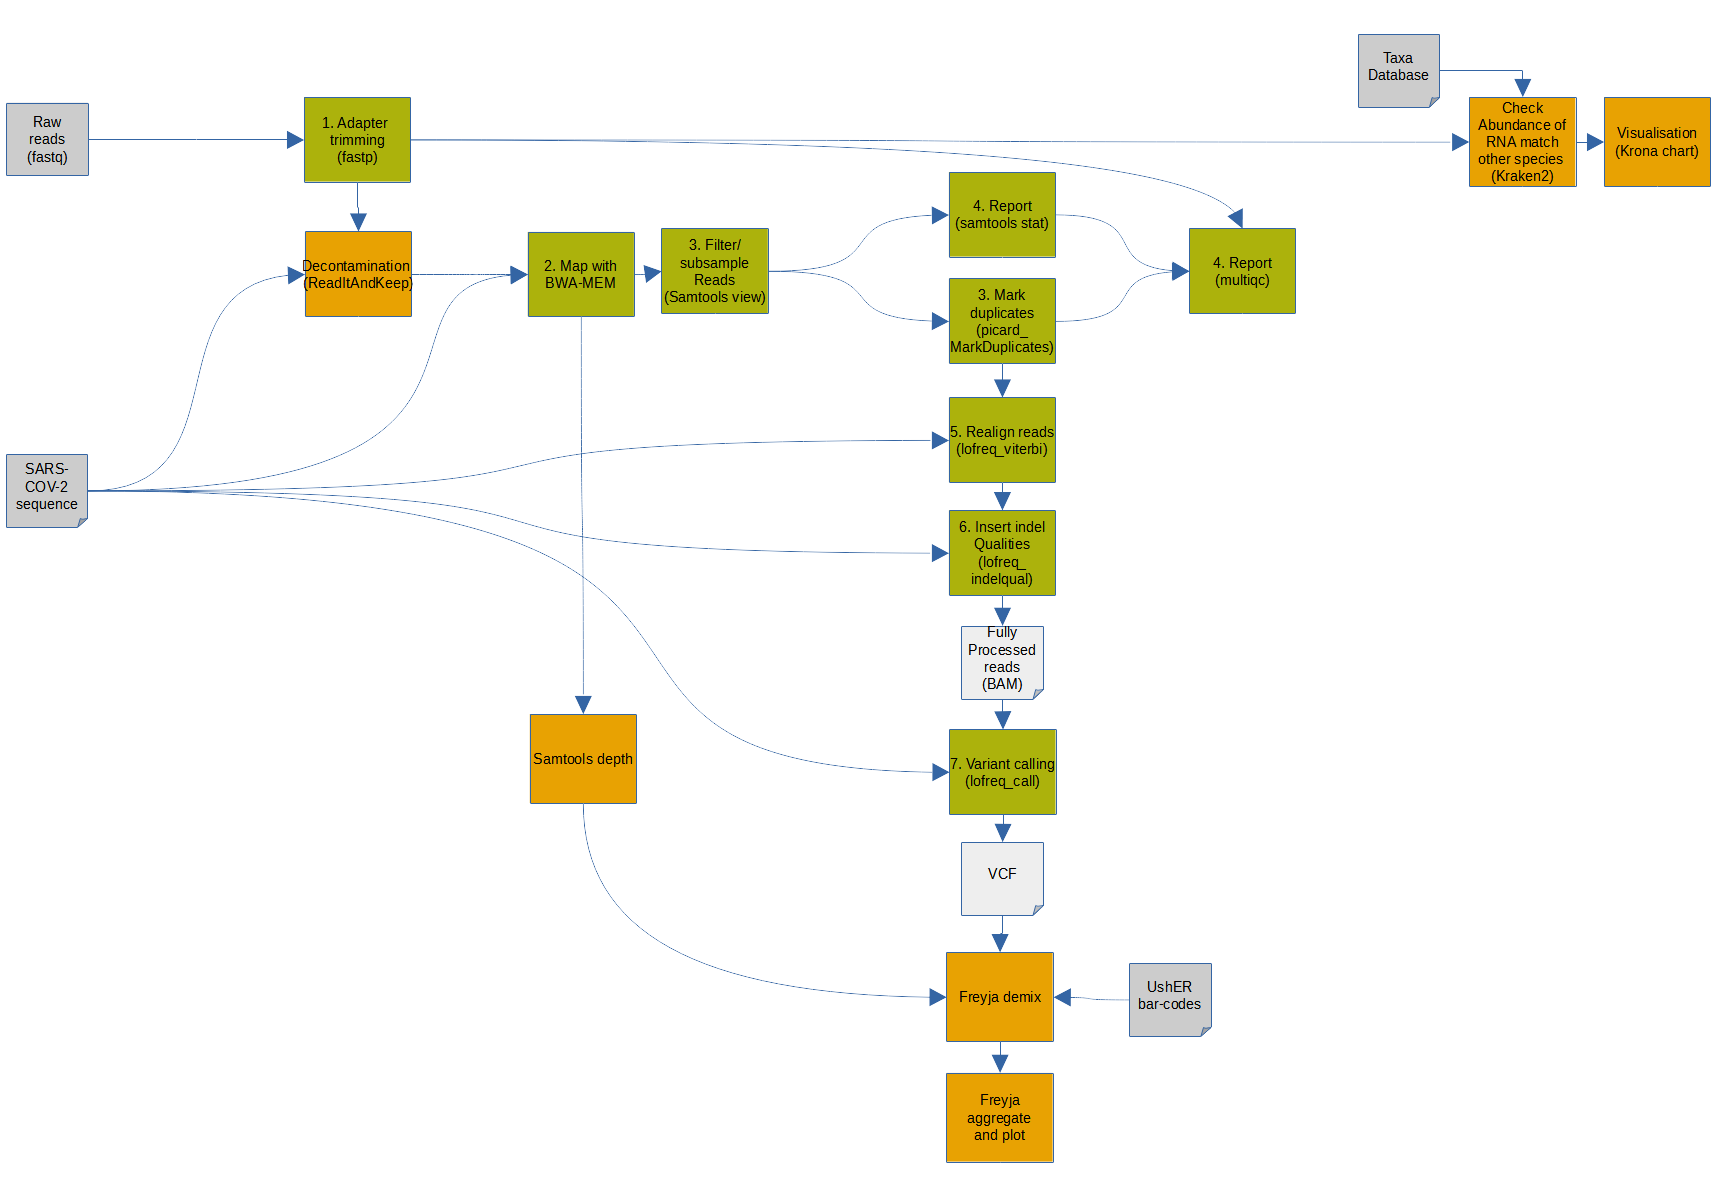
\includegraphics[width=1.3\textwidth]{figures/methods/metatranscriptomic-wf-after.png}
                \captionof{figure}{Improved and repurposed to SARS-CoV-2 wastewater surveillance Galaxy workflow for paired-end data extracted with metatranscriptomics-based technique and sequenced with Illumina sequencing approach.}
                \label{fig:methods:wgs-wf-after}
            \end{figure}
            \vfill
            \end{landscape}
        
    \subsection{Workflow evaluation} \label{sec:methods:evaluation}
    To assess the quality of developed workflows, I used a synthetically generated mock dataset and compared results obtained by the developed Galaxy workflow with expected ground truth results from the information about generated mock dataset. In addition, results from Galaxy workflow were benchmarked with the results from another solution, namely Lineagespot. Afterward, I launched both workflows on four real-world datasets mentioned in \cref{sec:methods:needs}.
        
        \subsubsection{Evaluation on mock data} \label{sec:methods:evaluation:mock}
            \paragraph{Generated mock datasets}
            Generated synthetic dataset was created by a working group and is uploaded in \href{https://github.com/suskraem/ww_benchmark}{Github repository} available under an open source license \cite{benchmarksamples}. Synthetic datasets were created by obtaining genomes from the Pango designation list. While generating synthetic mock data, the focus was on 3 real variants (BA.1, BA.2, Delta), one synthetic 'background' (BG) variant to mimic the effect of an unknown variant, as well as recombinant genomes (Omicron-Delta) \cite{simonloriere2011,variants}. Synthetic 'amplicons' were created using ARTIC v4.1 primers. Synthetic reads were created using error models based on 150 or 250bp NovaSeq reads. There were created samples belonging to groups of different classes such as: i) Single lineage, Two lineages, Three lineages; ii) High coverage, Low coverage; iii) Long reads, Short reads. In \cref{tab:methods:mock}, classes used to generate synthetic mock dataset are listed.
            
            \begin{table}[H]
            \centering
            \small
            \begin{tblr}{l|[dashed]llll}
            \textbf{Number}             & \textbf{Lineages}             & \textbf{Coverage}                   & \textbf{Read}          & \textbf{Number}  \\ 
            \textbf{of lineages}         &                              &                                     & \textbf{length, bp}           & \textbf{of samples} \\ \hline
            Single lineage          & BA.1                              & high                          & 150                               & 2 \\
                                    &                                   & low                           & 150                               & 2 \\
                                    &                                   &                               & 250                               & 2\\ \cline[dashed]{2-5}
                                    &  \textbf{BA.1 Total}              &                               &                                   & \textbf{8} \\\cline[dashed]{2-5}
                                    & BA.2                              & high                          & 150                               & 1 \\
                                    &                                   &                               & 250                               & 1 \\
                                    &                                   & low                           & 150                               & 1 \\
                                    &                                   &                               & 250                               & 1\\ \cline[dashed]{2-5}
                                    &  \textbf{BA.2 Total}              &                               &                                   & \textbf{4} \\\cline[dashed]{2-5}
                                    & Delta                              & high                          & 150                               & 1 \\
                                    &                                   &                               & 250                               & 1 \\
                                    &                                   & low                           & 150                               & 1 \\
                                    &                                   &                               & 250                               & 1\\ \cline[dashed]{2-5}
                                    &  \textbf{Delta Total}              &                               &                                   & \textbf{4} \\\cline[dashed]{2-5}
                                    &                                   &                               & 250                               & 1 \\
                                    &                                   &                               & 250                               & 1\\ \cline[dashed]{2-5}
                                    &  \textbf{Recombinant Total}       &                               &                                   & \textbf{2} \\\cline[dashed]{2-5}
                                    & Synthetic lineage                 & high                          & 150                               & 1 \\
                                    &                                   &                               & 250                               & 1 \\
                                    &                                   & low                           & 150                               & 1 \\
                                    &                                   &                               & 250                               & 1\\ \cline[dashed]{2-5}
                                    &  \textbf{Synthetic Total}         &                               &                                   & \textbf{4} \\\hline[dashed]
            \textbf{Single lineage Total} &                                  &                               &                                   & \textbf{22} \\ \hline
            Two                     & BA.1:BA.2                         & high                          & 250                               & 3 \\
             lineages               &                                   & low                           & 250                               & 3 \\\cline[dashed]{2-5}
                                    &  \textbf{BA.1:BA.2  Total}       &                               &                                   & \textbf{6} \\\cline[dashed]{2-5}
                                    & BA.1:Delta                         & high                          & 150                               & 7 \\
                                    &                                   &                               & 250                               & 14 \\
                                    &                                   & low                           & 150                               & 7 \\
                                    &                                   &                               & 250                               & 14\\ \cline[dashed]{2-5}
                                    &  \textbf{BA.1:Delta Total}        &                               &                                   & \textbf{42} \\\hline[dashed]
            \textbf{Two lineages}   &                                  &                               &                                   & \textbf{48} \\
            \textbf{Total}          &                                  &                               &                                   & \\\hline
             Two lineages           & BA.1:Delta:Synth                  & high                          & 250                               & 7 \\
            + Synthetic            &                                   & low                           & 250                               & 7 \\
             lineage               &                                   &                               &                                & \\ \hline[dashed]
                                    &  \textbf{BA.1:Delta:Synth Total}  &                               &                                   & \textbf{14} \\ \hline
            \end{tblr}
            \end{table}
            \begin{table}
            \begin{tblr}{l|[dashed]llll}
            \textbf{Number}             & \textbf{Lineages}             & \textbf{Coverage}                   & \textbf{Read}          & \textbf{Number}  \\ 
            \textbf{of lineages}         &                              &                                     & \textbf{length, bp}           & \textbf{of samples} \\ \hline
               Three                 &      BA.1:BA.2:Delta             &      high                         & 250                       & 4 \\
                lineages            &                                   &    low                           & 250                              & 4\\ \hline[dashed]
                                    &  \textbf{BA.1:BA.2:Delta Total}  &                               &                                   & \textbf{8} \\ \hline
                Three  lineages     &      BA.1:BA.2:Delta:Synth        &      high                     & 250                               & 4 \\
                + Synthetic          &                                   &    low                           & 250                           & 4\\ \hline[dashed]
                lineage              &  \textbf{BA.1:BA.2:Delta:Synth Total}  &                          &                                   & \textbf{8} \\ \hline
                \textbf{Total}      &                                    &                               &                                   & \textbf{100} \\ \hline

            \end{tblr}
                \caption{Overall numbers of samples, sorted by various groups of samples from the generated synthetically mock dataset. The table was created using a PivotTable in Google Sheets. Metadata about samples in the mock dataset was uploaded to Google Sheets, then, Pivot table was generated to analyze numerical data. First, data was sorted by Number of lineages, followed by sorting by exact Lineages combination, Coverage, and Read length. Next, the sum of samples for every class was calculated.} \label{tab:methods:mock}
            \end{table}

            Overall, the mock dataset contains 100 samples. More specifically, it contains 22 samples with single lineage, 42 with two distant lineages (BA.1 and Delta), 6 samples with two close lineages (BA.1 and BA.2), 14 samples with 2 known and one unknown lineage (synthetically generated), 8 samples with known lineages, and 8 samples with 3 known and one unknown lineages. In terms of coverage, the mock dataset contains 50 samples of low coverage and 50 samples of low coverage. In terms of read length, there are 24 samples of long reads (250 base pairs) and 76 samples of short reads (150 base pairs).
            
            In order to evaluate and draw conclusions about the performance and efficiency of developed workflows, the workflow for ampliconic-based data was run on a mock dataset along both branches: Freyja-based and COJAC-based. Aside from Galaxy, Lineagespot standalone workflow was launched in parallel on the same mock dataset for benchmarking all three methods' results.
            
            \paragraph{Comparison of proposed workflows} 
            To compare two branches of the proposed Galaxy workflow (with Freyja and with COJAC) and evaluate Galaxy workflow results, I examined them with the known expected results. Knowing the ground truth results allows me to draw conclusions about the performance of developed workflows and their accuracy. 
            
            For further evaluation, resulting data were divided according to the principle of belonging to a particular expected group. The groups of greatest interest were: Single lineage expected to be found in the sample and Two lineages.
            
            Even though both Freyja and COJAC methods found extra lineages that were not expected, I focused on their capability to detect expected lineages (Delta, BA.1, and BA.2) in abundance proportion closer to the expected proportion.

            
                \subparagraph{Preprocessing data} 
                Data obtained by Freyja and COJAC were preprocessed to make them comparable. Data from Freyja were obtained in \acrshort{tsv} (tabular) format (as shown for sample1 example in \cref{list:methods:freyja-s1}). To distinguish variants Delta, BA.1, and BA.2, which are focused on the mock dataset, a simple Python script (provided in \cref{list:methods:freyja-vocs-abundances}) was used considering that Delta lineage as B.1.617.2 and its sublineages starting with AY according to Pango designation \cite{otoole2021,covlineages}. In COJAC, in its turn, proportions of lineage abundances are computed for every amplicon, and for every lineage, a median of abundance proportion among different amplicons was computed.
                
                \begin{lstlisting}[language=xml, caption=Freyja output for sample 1 from mock dataset, label=list:methods:freyja-s1]
 Sample name	summarized	lineages	abundances	resid	coverage
 sample1 	[('Omicron', 0.6999889999983451), ('Delta', 0.22408099987442534), ('Other', 0.07552100018490182)]	BA.1.18 AY.4 BA.1.19 BA.1.1.13 BA.1.15.1 AY.38 BA.1.9 BA.1.16 B B.1.617.2 B.1.1.529 XS	0.23943700 0.11764700 0.11363600 0.10000000 0.09667000 0.06944400 0.06686400 0.06474800 0.06122400 0.03699000 0.01863400 0.01429700	7.611495978	99.95971667
                \end{lstlisting}
                
                To work with resulting output data from both branches of Galaxy workflow, they were stored in google sheets. Python pandas data analysis tool \cite{pandas2022} was used to access data and create dataframes from the data obtained. Dataframes were then used for downstream analysis.

                \subparagraph{Comparison}
                Parallel coordinates plot was created for detected proportions of different lineages using Python and Plotly graphing library \cite{plotly}. Three plots were generated for Delta, BA.1, and BA.2 lineages. First, I plotted all samples in one plot without their division into groups. All 100 samples were included in the first three plots in order to get an overall imagination of lineage proportion distribution among samples and their comparison to expected proportion values. Plots are available in \autoref{sec:appendix:figures:parallel-all} of \cref{sec:appendix}. The first axis is the Expected proportion, the second is the result obtained by COJAC, and finally, the third is Freyja’s proportion of the considered lineage of SARS-CoV-2. Additionally, I generated one plot per considered lineage (Delta, BA.1, or BA.2) and per group of samples (Single lineage expected, Two lineages expected). Overall, 6 plots were created. 

                To zoom up, the focus on one sample was done. Hence, there were generated for every sample: parallel coordinates plot and bar plot using Seaborn Python library, and line plot using Matplotlib (to look at absolute values of lineage proportion against scaled values in parallel coordinates). The comparison with expected lineage proportions was included in these plots.
                
                To compare Freyja and COJAC branches of workflow and to assess results with expected ones, I took a look at the distribution of Delta lineage proportion in the sample (obtained by Freyja, COJAC, and expected proportion) across all samples. The same comparison was made for BA.1 and BA.2 lineages.
                
                Other angle to look at results is to see a distribution of proportion of all three considered lineages across samples for both Freyja and COJAC. Thus, a distribution plot using Python and Seaborn library was generated. To be said, the similar distribution plot of proportion of all three considered lineages across samples for Lineagespot was generated analogously to plots for Freyja and COJAC.

                
            \paragraph{Comparison with lineagespot} \label{sec:methods:evaluation:mock:compare-ls}
            For the comparison of proposed Galaxy workflow results with Lineagespot results, the same synthetic mock dataset was used. Lineneagespot results on the mock dataset were obtained following private communication with F. Psomopoulos \cite{pechlivanis2022}. It was expected that the results of both branches of Galaxy workflow turned out to be different from the results of Lineagespot. That is because different approaches (sub-workflows) are used for the variant calling steps. In the case of Galaxy workflow, LoFreq variant caller is used preceding several steps for primer trimming, realignment, and insertion of indel qualities (using LoFreq\_insertindel). On the other hand, Lineagespot uses duplicates filtering with Picard tool, followed by variant calling with Freebayes tool. For lineage annotation, also different approaches are used. While for Galaxy workflow, Frejya or COJAC are options, Lineagespot pipeline uses its own approach for delineation. Thus, results from Galaxy workflow, whether Freyja-based or COJAC-based, are expected to differ.

            Data obtained from Lineagespot was already preprocessed, proportions of expected lineages were provided as well as assignments to certain lineages. To compare the results of Lineagespot and Galaxy workflows, Freyja-based or COJAC-based, against each other and against expected results, I focused specifically on two groups of samples from the mock dataset: the group where single lineage was expected (22 samples) and the group where two lineages were expected (48 samples). 

            
                \subparagraph{Single lineage group of samples} 
                For a single lineage group of samples, four characteristics were used. I intended to learn in which samples were detected: i) expected lineage; ii) expected+unexpected lineages; iii) unexpected lineage; iv) nothing. For each of these characteristics, bar plots were created separately, as well as a combined barplot that shows the number of samples that satisfy each characteristic. Also, a barplot was generated showing the percentage of samples that belong to each characteristic.

                Further, considering only samples where expected lineage was detected, the distribution of lineage proportion detected by Freyja and COJAC among samples of the Single lineage group was plotted with Python with the help of Seaborn library. Only Freyja and COJAC were compared. I do not consider Lineagespot here because in the results of Lineagespot I do not have a clean proportion distribution between lineages. There is no information about other lineages detected (aside from BA.1, BA.2, Delta), while the sum of proportions of these three is not equal to 1 in Lineagespot.
                
                To better understanding relationships between sets of different methods (Freyja, COJAC, Lineagespot) results, Venn Upset diagram was generated. The goal was to look at intersections between sets of results and which samples were detected correctly (in terms of lineages expected) by which tool and to find similarities in tools performance.

            
                \subparagraph{Two lineages group of samples}
                As for the group of samples where two lineages are expected to be found, I defined 5 characteristics depending on what was detected in samples: i) both expected lineages; ii) only one expected lineage; iii) one expected+unexpected lineages; iv) both expected+unexpected lineages; v) nothing. Similarly to the single lineage group of samples analysis, for each of these characteristics, barplots were created using Python separately as well as a combined barplot that shows the number of samples that satisfy each characteristic. Additionally, there was a barplot created showing the percentage of samples that belong to each characteristic.

                To zoom in, analysis was done for the most interesting sub-group of the group of samples where two lineages are expected to be detected. In this sub-group, there are two types of samples where both expected lineages are detected, and both expected + unexpected lineages are detected. To compare results, it is reasonable to look at the correlation between specific lineages, such as Delta, BA.1, and BA.2, as in this mock dataset, only three known lineages were used. The first option is to look at the ratio between BA.1 and BA.2 lineages. The second option is the relation between BA.1 and Delta lineages. The third is BA.2 and Delta relation. However, the third option does not make sense in this mock dataset because there are no samples in the group of two lineages where these two appear together at the same time.
                
                Therefore, in total, 6 cases were considered: i) BA1 > BA2; ii) BA1 = BA2; iii) BA1 < BA2; iv) BA1 > Delta;  v) BA1 = Delta;  vi) BA1 < Delta. 
                I looked at every case where this relation was expected and compared obtained results from Freyja, COJAC, and Lineagespot regarding the relation between two certain lineages (BA.1/BA.2 relation and BA.1/Delta relation). To visualize results, 6 bar plots were generated and explained in \cref{sec:results}.
                
                To better understand relationships between sets of different methods (Freyja, COJAC, Lineagespot) outputs, Venn Upset diagram was generated. The goal was to look at intersections between sets of results and in which samples both lineages were detected correctly (compared to expected ones) by which tool and to find similarities in tools' performance.
                
                All plots are shown in \cref{sec:results}.

        
        \subsubsection{Evaluation on real-world data} \label{sec:methods:evaluation:real}
        
            \paragraph{Chosen real-world datasets} 
            In order to provide a fairly comprehensive analysis, real-world datasets for experiments in this thesis were selected in such a way that they cover a variety of locations in the world and different time points of collecting samples. In this way, it was expected to obtain data on the evolution of SARS-CoV-2 over time, as well as data on which variants prevailed in which countries at these time points. This variety of datasets considered in this thesis can be in the future regularly analyzed using automatized Galaxy bot like it is currently managed for clinical data. 

            Choice of my thesis fell on the four datasets: i) one dataset from California (PRJNA661613)\cite{critschristoph} where the samples were collected in 2020 at a wastewater interceptor (labeled Berkeley, Berkeley Hills, Oakland, and Marin, according to the municipal areas each serves); ii) a dataset from the UK (PRJEB42191) \cite{hillary2021}, with data collected in sewage across six major urban centers in the UK (with a total population equivalent of 3 million) around the same time period (late spring - early summer of 2020) as the previous dataset  in order to show different proportions of different variants of the virus; iii) a dataset from wastewater treatment facilities across Ontario, Canada collected by Canadian Research Institute for Food Safety (PRJNA824537), which is interesting to analyze because it contains  one of the most recent datasets, the last sample was published in June of 2022; iv) a dataset from the US (PRJNA765346) collected by the FDA Center for Food Safety and Applied Nutrition \cite{nutrition2022}, one of the most extensive dataset with more than 340 samples already and regularly new samples are being added (last samples being from October of 2022). The exact data sources will be listed below.
            
            More metadata about datasets can be found in \cref{tab:methods:real-datasets}. Additionally, links to public Galaxy histories where datasets were analyzed with the proposed method are listed in \cref{sec:appendix:galaxy-hist}.
            \begin{landscape}
            \centering\vspace*{\fill}
                \begin{table}[ht!]
                \tiny
                \begin{tabular}{l|l|l|l|l|l|l|l|l|l|l|l}
                    \textbf{Location}&\textbf{Accession}&\textbf{Project}&\textbf{Description}&\textbf{Center name}&\multicolumn{1}{m{2cm}|}{\textbf{Sequencing platform}}&\multicolumn{1}{m{2cm}|}{\textbf{Library Strategy}}&\multicolumn{1}{m{2cm}|}{\textbf{Number of samples}}&\multicolumn{1}{m{2cm}|}{\textbf{\% of SARS-COV-2 on 3 randome samples}}&\multicolumn{1}{m{2cm}}{\textbf{Collection period}} \\
                    \hline 
                    \multicolumn{1}{m{1.5cm}|}{California, US}&SRP280174&\href{https://www.ebi.ac.uk/ena/browser/view/PRJNA661613}{PRJNA661613}&\multicolumn{1}{m{2cm}|}{California sewage metatranscriptomes enriched for respiratory viruses}&\multicolumn{1}{m{2cm}|}{Jill Banfield's Lab at Berkeley}&ILLUMINA&\multicolumn{1}{m{2cm}|}{Targeted-Capture}&11 (PE)&\multicolumn{1}{m{2cm}|}{0.74; 0.64; 0}&\multicolumn{1}{m{2cm}}{13.05.2020-30.06.2020} \\ \hline
                    \multicolumn{1}{m{1.5cm}|}{Wales and Northwest England, UK}&ERP126028&\href{https://www.ebi.ac.uk/ena/browser/view/PRJEB42191}{PRJEB42191}&\multicolumn{1}{m{2cm}|}{Monitoring SARS-CoV-2 in municipal wastewater to evaluate the success of lockdown measures for controlling COVID-19 in the UK}&\multicolumn{1}{m{2cm}|}{BANGOR UNIVERSITY}&ILLUMINA&\multicolumn{1}{m{2cm}|}{Ampliconic}&\multicolumn{1}{m{2cm}|}{340 (170-SE, 170-PE)}&\multicolumn{1}{m{2cm}|}{86.77; 95.15; 83.69}&\multicolumn{1}{m{2cm}}{30.03.2020-12.05.2020} \\\hline
                    \multicolumn{1}{m{1.5cm}|}{Ontario, Canada}&SRP368140&\href{https://www.ebi.ac.uk/ena/browser/view/PRJNA824537?show=reads}{PRJNA824537}&\multicolumn{1}{m{2cm}|}{Metagenomics analysis of wastewater influents from wastewater treatment facilities across Ontario}&\multicolumn{1}{m{2cm}|}{Canadian Research Institute for Food Safety}&ILLUMINA&\multicolumn{1}{m{2cm}|}{Ampliconic}&48 (PE)&\multicolumn{1}{m{2cm}|}{14.09}&\multicolumn{1}{m{2cm}}{29.11.2021-09.02.2022} \\\hline
                    \multicolumn{1}{m{1.5cm}|}{Washington, US}&SRP354651&\href{https://www.ebi.ac.uk/ena/browser/view/PRJNA765346}{PRJNA765346}&\multicolumn{1}{m{2cm}|}{GenomeTrakr wastewater project: Washington State Department of Health}&\multicolumn{1}{m{2cm}|}{FDA Center for Food Safety and Applied Nutrition}&ILLUMINA&\multicolumn{1}{m{2cm}|}{Ampliconic}&346 (PE)&\multicolumn{1}{m{2cm}|}{23.29; 18.79; 14.52}&\multicolumn{1}{m{2cm}}{25.11.2021-19.08.2022} \\
                    \hline
                \end{tabular}
                \caption{Real-world datasets used for this master thesis experiments. Datasets were downloaded from ENA database \cite{ena} with filters: i) sars-cov-2 and ii) wastewater. Four datasets, presented in this table, were chosen to be analyzed in this thesis considering a variety of locations and sample collection time.} \label{tab:methods:real-datasets}
                \end{table}
                \vfill
            \end{landscape}
            
            \paragraph{Comparison of proposed workflows}
            Both, Freyja and COJAC, generate a table-formatted file with results. Freyja, additionally, produces non-interactive and interactive plots. Non-interactive plots include 1) bar plots that show a fractional abundance estimate for all aggregated samples; 2) bar plots with sample collection time information with month binning and daily binning (when collection dates are provided)

            Freyja’s visualization has limitations. Freyja uses the UShER database to find lineages. Freyja creates plots based on WHO designations, like Omicron, Delta, etc. However, in the Californian (PRJNA661613) dataset, there are no exact WHO names defined in UShER. That means that for aggregation tables and for plotting Freyja uses the label “Other”. When detecting lineages that are considered by Freyja as “Other” designated name, the result bar plots are non-informative since they contain only one group of lineage - “Other”. Moreover, trying to produce an interactive dashboard, Freyja can meet an issue with “too many lineages to plot”. Freyja was able to produce interactive plots only for the UK (PRJEB42191) dataset, while for the rest, 3 out of 4 chosen real-world datasets, California (PRJNA661613), Canada (PRJNA824537), and US (PRJNA765346) ones, the issue with “too many lineages to plot” appeared.
            
            COJAC does not produce plots automatically, so bar plots similar to Freyja bar plots were generated using Python Matplotlib library to make a comparison for this thesis.

%%%%%%%%%%%%%%%%%%%%%%%%%%%%%%%%%%%%%%%%%%
% Master Thesis 
% Polina Polunina
% October 2022 
%
% License:
% CC-BY-SA 4.0 -- Creative Commons Attribution-ShareAlike 4.0 International
% https://creativecommons.org/licenses/by-sa/4.0/legalcode
%%%%%%%%%%%%%%%%%%%%%%%%%%%%%%%%%%%%%%%%%%
\section{Results}

\clearpage

%%%%%%%%%%%%%%%%%%%%%%%%%%%%%%%%%%%%%%%%%%
% Master Thesis 
% Polina Polunina
% October 2022 
%
% License:
% CC-BY-SA 4.0 -- Creative Commons Attribution-ShareAlike 4.0 International
% https://creativecommons.org/licenses/by-sa/4.0/legalcode
%%%%%%%%%%%%%%%%%%%%%%%%%%%%%%%%%%%%%%%%%%
\section{Discussion and Outlook}

\clearpage

%%%%%%%%%%%%%%%%%%%%%%%%%%%%%%%%%%%%%%%%%%
% Master Thesis 
% Polina Polunina
% October 2022 
%
% License:
% CC-BY-SA 4.0 -- Creative Commons Attribution-ShareAlike 4.0 International
% https://creativecommons.org/licenses/by-sa/4.0/legalcode
%%%%%%%%%%%%%%%%%%%%%%%%%%%%%%%%%%%%%%%%%%
\section{Appendix} \label{sec:appendix}
    \subsection{Galaxy histories} \label{sec:appendix:galaxy-hist}
    \subsubsection{Galaxy history links for Freyja-based branch on real datasets}
    California, US (PRJNA661613): \\
   \url{https://usegalaxy.eu/u/polina/h/sf-dataset-prjna661613-covid-19-variation-analysis-on-wgs-pe-data}\\
    Wales and Northwest England, UK (PRJEB42191): \\
    \url{https://usegalaxy.eu/u/polina/h/uk-dataset-COJAC-prjeb42191-covid-19-variation-analysis-on-artic-pe-data-1}\\
    Ontario, Canada (PRJNA824537): \\
    \url{https://usegalaxy.eu/u/polina/h/ca-dataset-freyja-prjna824537-covid-19-variation-analysis-on-artic-pe-data}\\
    Washington, US (PRJNA765346): \\
    \url{https://usegalaxy.eu/u/polina/h/us-dataset-freyja-prjna765346-covid-19-variation-analysis-on-artic-pe-data-1-1-1-1}

    \subsubsection{Galaxy history links for COJAC-based branch on real datasets}
    Wales and Northwest England, UK (PRJEB42191): \\
    \url{https://usegalaxy.eu/u/polina/h/uk-dataset-COJAC-prjeb42191-covid-19-variation-analysis-on-artic-pe-data-1}\\
    Ontario, Canada (PRJNA824537): \\
    \url{https://usegalaxy.eu/u/polina/h/ca-dataset-COJAC-prjna824537-covid-19-variation-analysis-on-artic-pe-data}\\
    Washington, US (PRJNA765346): \\
    \url{https://usegalaxy.eu/u/polina/h/us-dataset-COJAC-prjna765346-covid-19-variation-analysis-on-artic-pe-data}
    
    \subsection{Listings}
\begin{lstlisting}[language=bash, caption=macros for collection of related Freyja tool wrappers, label=list:methods:wrapper-freyja-macros]
<?xml version="1.0"?>
<macros>
    <token name="@TOOL_VERSION@">1.3.8</token>
    <token name="@VERSION_SUFFIX@">0</token>
    <token name="@PROFILE@">21.01</token>
    <xml name="biotools">
        <xrefs>
            <xref type="bio.tools">freyja</xref>
        </xrefs>
    </xml>
    <xml name="requirements">
        <requirements>
            <requirement type="package" version="@TOOL_VERSION@">freyja</requirement>
            <yield/>
        </requirements>
    </xml>
    <xml name="version">
        <version_command>freyja --version</version_command>
    </xml>
    <token name="@RUN_FREYJA_UPDATE_COMMAND@"><![CDATA[
#if $usher_update_option.choice == 'update'
    freyja update &&
#end if
]]></token>
    <token name="@PREPROCESS_VCF_INPUT@"><![CDATA[
ln -s '$variants_file' 'variants_file.vcf' &&
]]></token>
    <token name="@STANDARD_INPUT_FOR_BOOT@"><![CDATA[
#if $variants_file.ext == 'vcf'
    'variants_file.vcf'
#else
    '$variants_file'
#end if
'$depth_file'
#if $eps
    --eps '${eps}'
#end if
#if $meta
    --meta '${meta}'
#end if
$confirmedonly
]]></token>
    <token name="@CUSTOM_BARCODES_COMMAND@"><![CDATA[
#if $usher_update_option.choice == 'custom'
    --barcodes '${usher_update_option.usher_barcodes}'
#end if
]]></token>
    <token name="@DASH_COMMAND@"><![CDATA[
echo '${plot_format.plot_title}' > plot_title.txt &&
echo '${plot_format.plot_intro}' > plot_intro.txt &&
freyja dash
    #if $need_aggregation.choice == 'no'
        '$tsv_aggregated'
    #else
        'aggregated.tsv'
    #end if
    '$plot_format.csv_meta'
    plot_title.txt
    plot_intro.txt
    --output abundances_dashboard.html
]]></token>
    <token name="@PLOT_COMMAND@"><![CDATA[
freyja plot
    #if $need_aggregation.choice == 'no'
        '$tsv_aggregated'
    #else
        'aggregated.tsv'
    #end if
    --output abundances_plot.pdf
    #if $plot_format.csv_meta
        --times '${plot_format.csv_meta}'
    #end if
    #if $plot_format.interval == 'MS'
        --interval MS
    #else
        --interval D
        --windowsize 70
    #end if
]]></token>
    <token name="@PLOT_AND_DASH_COMMAND@"><![CDATA[
#if $plot_format.choice == 'dash'
    @DASH_COMMAND@
#else if $plot_format.choice == 'plot'
    freyja plot
    #if $need_aggregation.choice == 'no'
        $tsv_aggregated
    #else
        aggregated.tsv
    #end if
    --output abundances_plot.pdf
    #if $plot_format.need_metadata.choice == 'yes'
        --times '${plot_format.need_metadata.csv_meta}'
        #if $plot_format.need_metadata.interval == 'MS'
            --interval MS
        #else
            --interval D
            --windowsize 70
        #end if
    #end if
#else if $plot_format.choice == 'plot_and_dash'
    @DASH_COMMAND@ &&
    @PLOT_COMMAND@
#end if
]]></token>
    <xml name="demixing_common_options">
        <param name="depth_file" type="data" format="tabular" label="Sequencing depth file"/>
        <conditional name="usher_update_option">
            <param name="choice" type="select" label="Source of UShER barcodes data"
                   help="Freyja ships with an usher_barcodes.csv file, which the tool can access internally. Since this file gets updated rather frequently, you can also download the latest version of the file from https://github.com/andersen-lab/Freyja/raw/main/freyja/data/usher_barcodes.csv, set the dataset's datatype to csv and use it as a custom barcodes file.">
                <option value="repo" selected="true">Use data shipped with the tool (can be
                    outdated)
                </option>
                <option value="custom">Provide a custom barcodes file</option>
                <!--<option value="update">Get updated versions of the curated lineage file as well as the UShER global phylogenetic tree (can cause tool to run slowly)</option>-->
            </param>
            <when value="repo"/>
            <when value="custom">
                <param name="usher_barcodes" type="data" format="csv" label="UShER barcodes file"/>
            </when>
            <!--<when value="update" />-->
        </conditional>
        <param argument="--meta" type="data" format="json" optional="true"
               label="Custom lineage metadata file"
               help="For additional flexibility and reproducibility of analyses, a custom lineage-to-contellation mapping metadata file can be provided."/>
        <param argument="--eps" type="float" optional="true"
               label="Minimum lineage abundance tp include"
               help="e.g. 0.0001."/>
        <param argument="--confirmedonly" type="boolean" truevalue="--confirmedonly" falsevalue=""
               checked="false"
               label="Remove unconfirmed lineages from the analysis"
               help="If the UShER tree includes proposed lineages, the --confirmedonly flag removes unconfirmed lineages from the analysis."/>
    </xml>
    <token name="@HELP_HEADER@"><![CDATA[
What it does
============
Freyja is a tool to recover relative lineage abundances from mixed SARS-CoV-2 samples from a sequencing dataset (BAM aligned to the Hu-1 reference).
General information
===================
Freyja is a tool to recover relative lineage abundances from mixed SARS-CoV-2 samples from a sequencing dataset (BAM aligned to the Hu-1 reference). The method uses lineage-determining mutational "barcodes" derived from the UShER global phylogenetic tree as a basis set to solve the constrained (unit sum, non-negative) de-mixing problem.
Freyja is intended as a post-processing step after primer trimming and variant calling in iVar (Grubaugh and Gangavaparu et al., 2019). From measurements of SNV freqency and sequencing depth at each position in the genome, Freyja returns an estimate of the true lineage abundances in the sample.
]]></token>
    <xml name="citations">
        <citations>
            <citation type="doi">10.5281/zenodo.6585067</citation>
        </citations>
    </xml>
</macros>
\end{lstlisting}
\begin{lstlisting}[language=bash, caption=tool wrapper for Freyja: Call variants and get
sequencing depth information, label=list:methods:wrapper-freyja-call]
<tool id="freyja_variants" name="Freyja: Call variants"
      version="@TOOL_VERSION@+galaxy@VERSION_SUFFIX@"
      profile="@PROFILE@">
    <description>
        and get sequencing depth information
    </description>
    <macros>
        <import>macros.xml</import>
    </macros>
    <expand macro="biotools"/>
    <expand macro="requirements"/>
    <expand macro="version"/>
    <command detect_errors="exit_code"><![CDATA[
ln -s '$bam_file' 'bam_file' &&
ln -s '$ref_file' 'ref_file' &&
freyja variants 
    'bam_file'
    --variants variants 
    --depths '$depths'
    --ref 'ref_file'
    ]]></command>
    <inputs>
        <param name="bam_file" type="data" format="bam" label="BAM file"
               help="After primer trimming and alignment to reference genome."/>
        <param name="ref_file" argument="--ref" type="data" format="fasta"
               label="Reference sequence file"
               help="Note that the reference should match the fasta file used for alignment."/>
    </inputs>
    <outputs>
        <data name="variants" format="tabular" label="${tool.name} on ${on_string}: Variant call"
              from_work_dir="variants.tsv">
        </data>
        <data name="depths" format="tabular" label="${tool.name} on ${on_string}: Sequencing depth"
              from_work_dir="depths.tsv">
        </data>
    </outputs>
    <tests>
        <test expect_num_outputs="2">
            <param name="bam_file" value="test.bam"/>
            <param name="ref_file" value="NC_045512_Hu-1.fasta"/>
            <output name="variants" ftype="tabular">
                <assert_contents>
                    <has_text text="REF_CODON"/>
                    <has_text text="NC_045512.2"/>
                </assert_contents>
            </output>
            <output name="depths" ftype="tabular">
                <assert_contents>
                    <has_text text="NC_045512.2"/>
                </assert_contents>
            </output>
        </test>
    </tests>
    <help><![CDATA[
@HELP_HEADER@
Information about **freyja variants** method
============================================
The method uses both samtools and iVar. 
.. class:: warningmark
   Note that the reference should match the fasta file used for alignment. 
Outputs
=======
We get both variant call and sequencing depth information with this command.
    ]]></help>
    <expand macro="citations"/>
</tool>
\end{lstlisting}
\begin{lstlisting}[language=bash, caption=tool wrapper for Freyja: Bootstrapping method, label=list:methods:wrapper-freyja-boot]
<tool id="freyja_boot" name="Freyja: Bootstrapping" version="@TOOL_VERSION@+galaxy@VERSION_SUFFIX@"
      profile="@PROFILE@">
    <description>
        method
    </description>
    <macros>
        <import>macros.xml</import>
    </macros>
    <expand macro="biotools"/>
    <expand macro="requirements"/>
    <expand macro="version"/>
    <command detect_errors="exit_code"><![CDATA[
@RUN_FREYJA_UPDATE_COMMAND@
@PREPROCESS_VCF_INPUT@
freyja boot
    @STANDARD_INPUT_FOR_BOOT@
    --nt \${GALAXY_SLOTS:-4}
    #if $nb
        --nb $nb
    #end if
    --output_base 'boot_output'
    @CUSTOM_BARCODES_COMMAND@
    $boxplot_pdf
    ]]></command>
    <inputs>
        <param name="variants_file" type="data" format="tabular" label="Variants file"/>
        <expand macro="demixing_common_options"/>
        <param argument="--nb" type="integer" optional="true" label="Number of bootstraps"/>
        <param name="boxplot_pdf" argument="--boxplot pdf" type="boolean" truevalue="--boxplot pdf"
               falsevalue=""
               checked="false" label="Generate boxplot"/>
    </inputs>
    <outputs>
        <data name="boot_lineages" format="csv" label="${tool.name} on ${on_string}: Lineages"
              from_work_dir="boot_output_lineages.csv"/>
        <data name="boot_summarized" format="csv" label="${tool.name} on ${on_string}: Summarized"
              from_work_dir="boot_output_summarized.csv">
        </data>
        <data name="boot_lineages_plot" format="pdf"
              label="${tool.name} on ${on_string}: Lineages boxplot"
              from_work_dir="boot_output_lineages.pdf">
            <filter>boxplot_pdf</filter>
        </data>
        <data name="boot_summarized_plot" format="pdf"
              label="${tool.name} on ${on_string}: Summarized boxplot"
              from_work_dir="boot_output_summarized.pdf">
            <filter>boxplot_pdf</filter>
        </data>
    </outputs>
    <tests>
        <!-- Test 01: test tsv input files and plots -->
        <test expect_num_outputs="4">
            <conditional name="usher_update_option">
                <param name="choice" value="repo"/>
            </conditional>
            <param name="variants_file" value="variants.tsv"/>
            <param name="depth_file" value="depths.tsv"/>
            <param name="confirmedonly" value="false"/>
            <param name="nb" value="10"/>
            <param name="boxplot_pdf" value="true"/>
            <output name="boot_lineages" ftype="csv">
                <assert_contents>
                    <has_text text="B.1.617.2"/>
                </assert_contents>
            </output>
            <output name="boot_summarized" ftype="csv">
                <assert_contents>
                    <has_text text="Delta"/>
                </assert_contents>
            </output>
            <output name="boot_lineages_plot" ftype="pdf">
                <assert_contents>
                    <has_text text="Matplotlib"/>
                </assert_contents>
            </output>
            <output name="boot_summarized_plot" ftype="pdf">
                <assert_contents>
                    <has_text text="Matplotlib"/>
                </assert_contents>
            </output>
        </test>
        <!-- Test 02: test VCF input file -->
        <test expect_num_outputs="2">
            <conditional name="usher_update_option">
                <param name="choice" value="repo"/>
            </conditional>
            <param name="variants_file" value="test.vcf"/>
            <param name="depth_file" value="depths.tsv"/>
            <param name="confirmedonly" value="false"/>
            <param name="nb" value="10"/>
            <param name="boxplot_pdf" value="false"/>
            <output name="boot_lineages" ftype="csv">
                <assert_contents>
                    <has_text text="B.1.617.2"/>
                </assert_contents>
            </output>
            <output name="boot_summarized" ftype="csv">
                <assert_contents>
                    <has_text text="Delta"/>
                </assert_contents>
            </output>
        </test>
    </tests>
    <help><![CDATA[
@HELP_HEADER@
Information about **freyja boot** method
========================================
A fast bootstrapping method for freyja.
Outputs
=======
Bootstrapping method results:
1. Bootstrap lineages: the 0.025, 0.05,0.25,0.5 (median),0.75, 0.95, and 0.975 percentiles for each lineage;
2. Bootstrap summarized: WHO designated VOI/VOC
    ]]></help>
    <expand macro="citations"/>
</tool>
\end{lstlisting}
\begin{lstlisting}[language=bash, caption=tool wrapper for Freyja: Demix lineage abundances, label=list:methods:wrapper-freyja-demix]
<tool id="freyja_demix" name="Freyja: Demix" version="@TOOL_VERSION@+galaxy@VERSION_SUFFIX@"
      profile="@PROFILE@">
    <description>
        lineage abundances
    </description>
    <macros>
        <import>macros.xml</import>
    </macros>
    <expand macro="biotools"/>
    <expand macro="requirements">
        <requirement type="package" version="4.7">sed</requirement>
    </expand>
    <expand macro="version"/>
    <command detect_errors="exit_code"><![CDATA[
@RUN_FREYJA_UPDATE_COMMAND@
#if str($sample_name.source) == 'auto':
    #set $sn = $variants_in.element_identifier
#else:
    #set $sn = str($sample_name.name)
#end if
#set $in_file = $sn.replace(' ', '_') + '.' + $variants_in.ext
ln -s '$variants_in' $in_file &&
freyja demix
    '$in_file'
    '$depth_file'
    #if $eps
        --eps $eps
    #end if
    #if $meta
        --meta '$meta'
    #end if
    $confirmedonly
    @CUSTOM_BARCODES_COMMAND@
    --covcut $depth_cutoff
    --output abundances_raw.tsv &&
sed 's/$in_file/$sn/' abundances_raw.tsv > abundances.tsv
    ]]></command>
    <inputs>
        <param name="variants_in" type="data" format="tabular"
               label="Dataset with input variant calls"
               help="This can be a VCF dataset, or the tabular calls output of freayja call or ivar variants."/>
        <conditional name="sample_name">
            <param name="source" type="select" label="Set sample name"
                   help="Select autodetect to have the dataset or collection element name used as the sample name, or, for a single input dataset, provide an explicit sample name.">
                <option value="auto">Autodetect sample name</option>
                <option value="manual">Specify sample name explicitly</option>
            </param>
            <when value="auto"/>
            <when value="manual">
                <param name="name" type="text" label="Name of the sample"/>
            </when>
        </conditional>
        <expand macro="demixing_common_options"/>
        <param name="depth_cutoff" argument="--covcut" type="integer" min="0" value="10"
               multiple="true"
               label="Depth cutoff for coverage estimate"
               help="In the result file the coverage value will provide the 10x coverage estimate (percent of sites with 10 or greater reads- 10 is the default but can be modfied in this field. "/>
    </inputs>
    <outputs>
        <data name="abundances" format="tabular"
              label="${tool.name} on ${on_string}: Lineages abundances summary"
              from_work_dir="abundances.tsv"/>
    </outputs>
    <tests>
        <!-- Test 01: manual name sample -->
        <test expect_num_outputs="1">
            <param name="variants_in" value="variants.tsv"/>
            <param name="depth_file" value="depths.tsv"/>
            <conditional name="usher_update_option">
                <param name="choice" value="repo"/>
            </conditional>
            <conditional name="sample_name">
                <param name="source" value="manual"/>
                <param name="name" value="samplename"/>
            </conditional>
            <output name="abundances" ftype="tabular">
                <assert_contents>
                    <has_text text="samplename"/>
                </assert_contents>
            </output>
        </test>
        <!-- Test 02: autoname sample -->
        <test expect_num_outputs="1">
            <param name="variants_in" value="variants.tsv"/>
            <param name="depth_file" value="depths.tsv"/>
            <conditional name="usher_update_option">
                <param name="choice" value="repo"/>
            </conditional>
            <conditional name="sample_name">
                <param name="source" value="auto"/>
            </conditional>
            <output name="abundances" ftype="tabular">
                <assert_contents>
                    <has_text text="summarized"/>
                </assert_contents>
            </output>
        </test>
    </tests>
    <help><![CDATA[
@HELP_HEADER@
**Freyja demix** estimates lineage abundances in a potentially multi-lineage input sample.
Inputs
======
The tool requires as input a dataset with called variants and a dataset with genome-wide sequencing depth information.
Both types of data can be produced with *Freyja call*, but the tool accepts variant calls also in VCF format.
Note
----
For single samples it is recommended to select "Specify sample name explicitly"
under "Set sample name".
To use this tool on multiple samples in parallel, please provide two
collections in the same sample sort order - one with the variant calls, the
other one with the sequencing depths - and select "Autodetect sample name",
which will use collection element identifiers as the names of the samples.
This will produce a new collection of demixing reports that can be passed to
*Freyja: Aggregate and visualize* with sample names preserved.
Selection of multiple regular called variants and depth datasets is discouraged
since proper dataset pairing cannot be guaranteed!
Outputs
=======
The tool produces tabular output that includes the lineages detected in the sample, their corresponding abundances, and a lineage summary by constellation.
Example output:
========== ===================================================
           filename
summarized [('Delta', 0.65), ('Other', 0.25), ('Alpha', 0.1')] 
lineages   ['B.1.617.2' 'B.1.2' 'AY.6' 'Q.3']
abundances "[0.5 0.25 0.15 0.1]"
resid      3.14159
coverage   95.8
========== ===================================================
Where *summarized* denotes a sum of all lineage abundances in a particular WHO designation (i.e. B.1.617.2 and AY.6 abundances are summed in the above example), otherwise they are grouped into "Other". The *lineage* array lists the identified lineages in descending order, and *abundances* contains the corresponding abundances estimates. The value of *resid* corresponds to the residual of the weighted least absolute devation problem used to estimate lineage abundances. The *coverage* value provides the 10x coverage estimate (percent of sites with 10 or greater reads- 10 is the default but can be modfied using the *--covcut* option).
    ]]></help>
    <expand macro="citations"/>
</tool>
\end{lstlisting}
\begin{lstlisting}[language=bash, caption=tool wrapper for Freyja: Aggregate and visualize demixed results, label=list:methods:wrapper-freyja-agg]
<tool id="freyja_aggregate_plot" name="Freyja: Aggregate and visualize"
      version="@TOOL_VERSION@+galaxy@VERSION_SUFFIX@"
      profile="@PROFILE@">
    <description>
        demixed results
    </description>
    <macros>
        <import>macros.xml</import>
    </macros>
    <expand macro="biotools"/>
    <expand macro="requirements"/>
    <expand macro="version"/>
    <command detect_errors="exit_code"><![CDATA[
#if $need_aggregation.choice == 'yes'
    #set demix_dir = 'demix_outputs/'
    #set file_paths1 = []
    mkdir -p demix_outputs &&
    #for $input_file in $demix_file
        #set $file_path = $demix_dir + $input_file.element_identifier
        ln -s '$input_file' '$file_path' &&
        $file_paths1.append($file_path)
    #end for
    freyja aggregate
        '$demix_dir'
        --output aggregated.tsv
    #if $plot_format.choice != 'none'
        &&
    #end if
#end if
@PLOT_AND_DASH_COMMAND@
    ]]></command>
    <inputs>
        <conditional name="need_aggregation">
            <param name="choice" type="select"
                   label="Aggregate demixed data or provide aggregated data file?">
                <option value="yes">aggregate demixed data</option>
                <option value="no">provide aggregated data file</option>
            </param>
            <when value="yes">
                <param name="demix_file" type="data" format="tabular" multiple="true"
                       label="Lineages abundances summary file(s)" help="One file per one sample."/>
            </when>
            <when value="no">
                <param name="tsv_aggregated" type="data" format="tabular"
                       label="Provide aggregated data"/>
            </when>
        </conditional>
        <conditional name="plot_format">
            <param name="choice" type="select" label="Report(s) to generate">
                <option value="plot">non-interactive plot</option>
                <option value="dash">interactive dashboard (html)</option>
                <option value="plot_and_dash">plot and dashboard</option>
                <option value="none">no plots, just aggregated data table</option>
            </param>
            <when value="plot">
                <conditional name="need_metadata">
                    <param name="choice" type="select"
                           label="Provide a sample metadata file for plotting data over time?">
                        <option value="yes">Yes</option>
                        <option value="no">No</option>
                    </param>
                    <when value="yes">
                        <param name="csv_meta" type="data" format="csv"
                               label="Provide time(s) metadata file"
                               help="See info box below to learn more about the form of meta-file. Accepts only CSV (.csv) files"/>
                        <param name="interval" type="select" label="Choose interval" display="radio"
                               help="Used for pdf format.">
                            <option value="MS" selected="true">month bins</option>
                            <option value="D">day bins</option>
                        </param>
                    </when>
                    <when value="no"/>
                </conditional>
            </when>
            <when value="dash">
                <param name="csv_meta" type="data" format="csv"
                       label="Provide sample(s) metadata file"
                       help="See info box below to learn more about the form of meta-file. Accepts only CSV (.csv) files"/>
                <param name="plot_title" type="text" value="" optional="true" label="Title"/>
                <param name="plot_intro" type="text" value="" optional="true" label="Introduction"/>
            </when>
            <when value="plot_and_dash">
                <param name="csv_meta" type="data" format="csv"
                       label="Provide sample(s)/time(s) metadata file"
                       help="See info box below to learn more about the form of meta-file. Accepts only CSV (.csv) files"/>
                <param name="plot_title" type="text" value="" optional="true" label="Title"
                       help="Used for interactive dashboard."/>
                <param name="plot_intro" type="text" value="" optional="true" label="Introduction"
                       help="Used for interactive dashboard."/>
                <param name="interval" type="select" label="Choose interval" display="radio"
                       help="Used for pdf non-interactive plot.">
                    <option value="MS" selected="true">month bins</option>
                    <option value="D">day bins</option>
                </param>
            </when>
            <when value="none"/>
        </conditional>
    </inputs>
    <outputs>
        <!-- outputs for aggregate command -->
        <data name="aggregated" format="tabular"
              label="${tool.name} on ${on_string}: Aggregated data"
              from_work_dir="aggregated.tsv">
            <filter>need_aggregation['choice'] == 'yes'</filter>
        </data>
        <!-- outputs for dash command -->
        <data name="abundances_dashboard" format="html"
              label="${tool.name} on ${on_string}: Lineages abundances dashboard"
              from_work_dir="abundances_dashboard.html">
            <filter>plot_format['choice'] == 'dash' or plot_format['choice'] == 'plot_and_dash'
            </filter>
        </data>
        <!-- outputs for plot command -->
        <data name="abundances_plot" format="pdf"
              label="${tool.name} on ${on_string}: Lineages abundances plot"
              from_work_dir="abundances_plot.pdf">
            <filter>plot_format['choice'] == 'plot' or plot_format['choice'] == 'plot_and_dash'
            </filter>
        </data>
    </outputs>
    <tests>
        <!-- Test 01: aggregate command -->
        <test expect_num_outputs="1">
            <conditional name="need_aggregation">
                <param name="choice" value="yes"/>
                <param name="demix_file"
                       value="abundances.tsv,abundances2.tsv,abundances3.tsv,abundances4.tsv"/>
            </conditional>
            <conditional name="plot_format">
                <param name="choice" value="none"/>
            </conditional>
            <output name="aggregated" ftype="tabular">
                <assert_contents>
                    <has_text text="summarized"/>
                    <has_text text="abundances"/>
                    <has_text text="B.1.617.2"/>
                </assert_contents>
            </output>
        </test>
        <!-- Test 02: dash command -->
        <test expect_num_outputs="1">
            <conditional name="need_aggregation">
                <param name="choice" value="no"/>
                <param name="tsv_aggregated" value="bunch_of_files.tsv"/>
            </conditional>
            <conditional name="plot_format">
                <param name="choice" value="dash"/>
                <param name="csv_meta" value="csv_sample_meta.csv"/>
                <param name="plot_title" value="This is title"/>
                <param name="plot_intro" value="Local WW Dashboard"/>
            </conditional>
            <output name="abundances_dashboard" ftype="html">
                <assert_contents>
                    <has_text text="Local WW Dashboard"/>
                </assert_contents>
            </output>
        </test>
        <!-- Test 03: plot command -->
        <test expect_num_outputs="1">
            <conditional name="need_aggregation">
                <param name="choice" value="no"/>
                <param name="tsv_aggregated" value="bunch_of_files.tsv"/>
            </conditional>
            <conditional name="plot_format">
                <param name="choice" value="plot"/>
                <conditional name="need_metadata">
                    <param name="choice" value="yes"/>
                    <param name="csv_meta" value="times_metadata.csv"/>
                    <param name="interval" value="D"/>
                </conditional>
            </conditional>
            <output name="abundances_plot" ftype="pdf">
                <assert_contents>
                    <has_text text="Matplotlib"/>
                </assert_contents>
            </output>
        </test>
        <!-- Test 04: aggregate and dash commands -->
        <test expect_num_outputs="2">
            <conditional name="need_aggregation">
                <param name="choice" value="yes"/>
                <param name="demix_file" value="abundances.tsv,abundances2.tsv,abundances3.tsv"/>
            </conditional>
            <conditional name="plot_format">
                <param name="choice" value="dash"/>
                <param name="csv_meta" value="csv_sample_meta2.csv"/>
                <param name="plot_title" value="This is title"/>
                <param name="plot_intro" value="Local WW Dashboard"/>
            </conditional>
            <output name="aggregated" ftype="tabular">
                <assert_contents>
                    <has_text text="summarized"/>
                    <has_text text="abundances"/>
                    <has_text text="B.1.617.2"/>
                </assert_contents>
            </output>
            <output name="abundances_dashboard" ftype="html">
                <assert_contents>
                    <has_text text="Local WW Dashboard"/>
                </assert_contents>
            </output>
        </test>
        <!-- Test 05: aggregate and plot commands -->
        <test expect_num_outputs="2">
            <conditional name="need_aggregation">
                <param name="choice" value="yes"/>
                <param name="demix_file" value="abundances.tsv,abundances2.tsv,abundances3.tsv"/>
            </conditional>
            <conditional name="plot_format">
                <param name="choice" value="plot"/>
                <conditional name="need_metadata">
                    <param name="choice" value="yes"/>
                    <param name="csv_meta" value="csv_sample_meta2.csv"/>
                    <param name="interval" value="D"/>
                </conditional>
            </conditional>
            <output name="aggregated" ftype="tabular">
                <assert_contents>
                    <has_text text="summarized"/>
                    <has_text text="abundances"/>
                    <has_text text="B.1.617.2"/>
                </assert_contents>
            </output>
            <output name="abundances_plot" ftype="pdf">
                <assert_contents>
                    <has_text text="Matplotlib"/>
                </assert_contents>
            </output>
        </test>
        <!-- Test 06: aggregate, dash and plot commands -->
        <test expect_num_outputs="3">
            <conditional name="need_aggregation">
                <param name="choice" value="yes"/>
                <param name="demix_file" value="abundances.tsv,abundances2.tsv,abundances3.tsv"/>
            </conditional>
            <conditional name="plot_format">
                <param name="choice" value="plot_and_dash"/>
                <param name="csv_meta" value="csv_sample_meta2.csv"/>
                <param name="plot_title" value="This is title"/>
                <param name="plot_intro" value="Local WW Dashboard"/>
                <param name="interval" value="D"/>
            </conditional>
            <output name="aggregated" ftype="tabular">
                <assert_contents>
                    <has_text text="summarized"/>
                    <has_text text="abundances"/>
                    <has_text text="B.1.617.2"/>
                </assert_contents>
            </output>
            <output name="abundances_plot" ftype="pdf">
                <assert_contents>
                    <has_text text="Matplotlib"/>
                </assert_contents>
            </output>
            <output name="abundances_dashboard" ftype="html">
                <assert_contents>
                    <has_text text="Local WW Dashboard"/>
                </assert_contents>
            </output>
        </test>
    </tests>
    <help><![CDATA[
@HELP_HEADER@

Information about **freyja aggregate** method
=============================================

Method for manipulating the "demixed" output files. 

Outputs
-------

This resulting aggregated data can analyzed directly as a tsv file, or can be visualized using *freyja plot* and *freyja dash*.

Information about **freyja plot** method
========================================

Method provides a fractional abundance estimate for all aggregated samples.

A **time(s) metadata CSV file** should have this form:

*Sample,sample_collection_datetime*  

*sample_0.tsv,03/01/21*  

*sample_1.tsv,03/03/21*  
 
*sample_2.tsv,03/08/21*  

*sample_3.tsv,03/10/21*  

*sample_4.tsv,03/12/21*  

*sample_5.tsv,03/14/21*  

*sample_6.tsv,03/17/21*  

*sample_7.tsv,03/20/21*  

*sample_8.tsv,03/25/21*  

*sample_9.tsv,03/30/21*  

*sample_10.tsv,03/31/21*  

*sample_11.tsv,04/04/21*


Information about **freyja dash** method
========================================

Functionality to rapidly prepare a dashboard web page, directly from aggregated freyja output.

A **sample(s) metadata CSV file** should have this form:

*Sample,sample_collection_datetime,viral_load*  

*sample_0.tsv,03/01/21,460326*  

*sample_1.tsv,03/03/21,176645.1*  

*sample_2.tsv,03/08/21,449891.7*  

*sample_3.tsv,03/10/21,361699.5*  

*sample_4.tsv,03/12/21,658923.9*  

*sample_5.tsv,03/14/21,500432.8*  

*sample_6.tsv,03/17/21,791406.4*  

*sample_7.tsv,03/20/21,628119.9*  

*sample_8.tsv,03/25/21,810673.9*  

*sample_9.tsv,03/30/21,1263564.4*  

*sample_10.tsv,03/31/21,1627556.3*  

*sample_11.tsv,04/04/21,1528006.4*


    ]]></help>
    <expand macro="citations"/>
</tool>
\end{lstlisting}

\begin{lstlisting}[language=bash, caption=macros for collection of related Freyja tool wrappers, label=list:methods:wrapper-cojac-macros]
<?xml version="1.0"?>
<macros>
    <token name="@TOOL_VERSION@">0.2</token>
    <token name="@VERSION_SUFFIX@">0</token>
    <token name="@PROFILE@">21.01</token>
    <xml name="biotools">
        <xrefs>
            <xref type="bio.tools">cojac</xref>
        </xrefs>
    </xml>
    <xml name="requirements">
        <requirements>
            <requirement type="package" version="@TOOL_VERSION@">cojac</requirement>
            <yield/>
        </requirements>
    </xml>
    <xml name="version">
        <version_command>echo @TOOL_VERSION@</version_command>
    </xml>
    <xml name="vocdir_input">
        <conditional name="vocdir_option">
            <param name="choice" type="select"
                   label="Source of YAML files with definition of the variant of concerns"
                   help="Cojac ships with a directory with variant definitions yaml files (https://github.com/cbg-ethz/cojac/tree/master/voc), which the tool can access internally. You can also download the latest version of the yaml files from https://github.com/phe-genomics/variant_definitions and use it as a custom yamls defining the variant of concerns.">
                <option value="cache">Definitions shipped with the tool (can be outdated)</option>
                <option value="custom">From history</option>
            </param>
            <when value="cache"/>
            <when value="custom">
                <param name="voc_file" type="data" format="yaml" multiple="true"
                       label="YAML defining the variant of concern"/>
            </when>
        </conditional>
    </xml>
    <token name="@VOCDIR_COMMAND@"><![CDATA[
#if $vocdir_option.choice == 'custom'
    #set vocdir = 'voc/'
    #set file_paths1 = []
    mkdir -p voc &&
    #for $input_file in $voc_file
        #set $file_path = $vocdir + $input_file.element_identifier
        ln -s '$input_file' '$file_path' &&
        $file_paths1.append($file_path)
    #end for
#else
    DB_PATH="\$(dirname "\$(dirname "\$(which cooc-mutbamscan)")")/share/cojac" &&
    ln -s "\$DB_PATH" db &&
    #set $vocdir = 'db/voc'
#end if
]]></token>
    <token name="@HELP_HEADER@"><![CDATA[
What it does
============

The cojac package comprises a set of command-line tools to analyse co-occurrence of mutations on amplicons. It is useful, for example, for early detection of viral variants of concern (e.g. Alpha, Delta, Omicron) in environmental samples, and has been designed to scan for multiple SARS-CoV-2 variants in wastewater samples.
]]></token>
    <xml name="citations">
        <citations>
            <citation type="doi">10.1101/2021.01.08.21249379</citation>
        </citations>
    </xml>
</macros>
\end{lstlisting}
\begin{lstlisting}[language=bash, caption=tool wrapper for Cojac: mutbamscan, label=list:methods:wrapper-cojac-mutbamcsan]
<tool id="cooc_mutbamscan" name="Cojac: mutbamscan" version="@TOOL_VERSION@+galaxy@VERSION_SUFFIX@"
      profile="@PROFILE@">
    <description>
        scan an alignment file for mutation co-occurrences
    </description>
    <macros>
        <import>macros.xml</import>
    </macros>
    <expand macro="biotools"/>
    <expand macro="requirements"/>
    <expand macro="version"/>
    <command detect_errors="exit_code"><![CDATA[
ln -s '$bed_file' 'bed_file' &&
@VOCDIR_COMMAND@
#import re
#set identifier = re.sub('[^\s\w\-\\.]', '_', str($bam_file.element_identifier))
ln -s '$bam_file' ${identifier}.bam &&
ln -s '${bam_file.metadata.bam_index}' ${identifier}.bai &&
cooc-mutbamscan
    -a '${identifier}.bam'
    -b 'bed_file'
    -m '$vocdir'
    -y cooc.yaml
    -j cooc.json
    #if $amplicons_file.choice == 'build'
        -A amplicons.yaml
    #else
        -Q '$amplicons_file.in_amp'
    #end if
    -t cooc.tsv
    --cooc $cooc
    ]]></command>
    <inputs>
        <expand macro="vocdir_input"/>
        <param name="bed_file" type="data" format="bed"
               label="BED file defining the amplicons"/>
        <param name="bam_file" type="data" format="bam,cram,sam"
               label="Alignment BAM/CRAM/SAM file"/>
        <param argument="--cooc" type="integer" min="1" value="2"
               label="Minimum number of cooccurence mutations on the same amplicon"/>
        <conditional name="amplicons_file">
            <param name="choice" type="select" label="Source of amplicons YAML file">
                <option value="build">Build from BED + set of YAMLs for variants of concern</option>
                <option value="custom">From history</option>
            </param>
            <when value="build"/>
            <when value="custom">
                <param name="in_amp" type="data" format="yaml"
                       label="YAML file to query amplicons"/>
            </when>
        </conditional>
        <param name="output_files" type="select" display="checkboxes"
               multiple="true" label="Output files">
            <option value="yaml" selected="true">YAML</option>
            <option value="json">JSON</option>
            <option value="tabular">tabular</option>
        </param>
    </inputs>
    <outputs>
        <data name="cooc_yaml" format="yaml"
              label="${tool.name} on ${on_string}: Mutation cooccurrence (yaml)"
              from_work_dir="cooc.yaml">
            <filter>'yaml' in output_files</filter>
        </data>
        <data name="cooc_json" format="json"
              label="${tool.name} on ${on_string}: Mutation cooccurrence (json)"
              from_work_dir="cooc.json">
            <filter>'json' in output_files</filter>
        </data>
        <data name="cooc_tsv" format="tabular"
              label="${tool.name} on ${on_string}: Mutation cooccurrence (tabular)"
              from_work_dir="cooc.tsv">
            <filter>'tabular' in output_files</filter>
        </data>
        <data name="amplicons" format="yaml"
              label="${tool.name} on ${on_string}: Amplicons (yaml)"
              from_work_dir="amplicons.yaml">
            <filter>amplicons_file['choice'] == 'build'</filter>
        </data>
    </outputs>
    <tests>
        <!-- Test 1: build yaml for amplicons from bed and voc/ -->
        <test expect_num_outputs="4">
            <conditional name="vocdir_option">
                <param name="choice" value="custom"/>
                <param name="voc_file" value="omicron_ba1_mutations.yaml"/>
            </conditional>
            <param name="bam_file" value="tbam11.bam"/>
            <param name="bed_file" value="nCoV-2019.insert.V3.bed"/>
            <conditional name="amplicons_file">
                <param name="choice" value="build"/>
            </conditional>
            <param name="output_files" value="yaml,json,tabular"/>
            <output name="cooc_yaml" ftype="yaml">
                <assert_contents>
                    <has_text text="76_om1"/>
                    <has_text text="81_om1"/>
                </assert_contents>
            </output>
            <output name="cooc_json" ftype="json">
                <assert_contents>
                    <has_text text="76_om1"/>
                    <has_text text="81_om1"/>
                </assert_contents>
            </output>
            <output name="cooc_tsv" ftype="tabular">
                <assert_contents>
                    <has_text text="76_om1"/>
                    <has_text text="81_om1"/>
                </assert_contents>
            </output>
            <output name="amplicons" ftype="yaml">
                <assert_contents>
                    <has_text text="76_om1"/>
                    <has_text text="81_om1"/>
                </assert_contents>
            </output>
        </test>
        <!-- Test 2: supply yaml for amplicons and voc/ from cache -->
        <test expect_num_outputs="2">
            <conditional name="vocdir_option">
                <param name="choice" value="cache"/>
            </conditional>
            <param name="bam_file" value="tbam11.bam"/>
            <param name="bed_file" value="nCoV-2019.insert.V3.bed"/>
            <conditional name="amplicons_file">
                <param name="choice" value="custom"/>
                <param name="in_amp" value="amplicons111.yaml"/>
            </conditional>
            <param name="output_files" value="yaml,tabular"/>
            <output name="cooc_yaml" ftype="yaml">
                <assert_contents>
                    <has_text text="76_om1"/>
                    <has_text text="81_om1"/>
                </assert_contents>
            </output>
            <output name="cooc_tsv" ftype="tabular">
                <assert_contents>
                    <has_text text="76_om1"/>
                    <has_text text="81_om1"/>
                </assert_contents>
            </output>
        </test>
    </tests>
    <help><![CDATA[
@HELP_HEADER@

Information about **cooc-mutbamscan** method
============================================

The method scans an alignment BAM/CRAM/SAM file for mutation co-occurrences and output a JSON or YAML file.

    ]]></help>
    <expand macro="citations"/>
</tool>
\end{lstlisting}
\begin{lstlisting}[language=bash, caption=tool wrapper for Cojac: tabmut, label=list:methods:wrapper-cojac-tabmut]
<tool id="cooc_tabmut" name="Cojac: tabmut" version="@TOOL_VERSION@+galaxy@VERSION_SUFFIX@"
      profile="@PROFILE@">
    <description>
        export cooccurrence mutations as a table
    </description>
    <macros>
        <import>macros.xml</import>
    </macros>
    <expand macro="biotools"/>
    <expand macro="requirements"/>
    <expand macro="version"/>
    <command detect_errors="exit_code"><![CDATA[
#for $input_file in $cooc_file
    #set $cooc_ext = $input_file.ext
#end for
cooc-tabmut
    #if $cooc_ext == 'json'
        -j '$cooc_file'
    #else if $cooc_ext == 'yaml'
        -y '$cooc_file'
    #end if
    -o cooc-table.csv
    #if $table_orientation.choice == 'lines'
        -l
    #else if $table_orientation.choice == 'multiindex'
        -m
    #end if
    -q
    ]]></command>
    <inputs>
        <param name="cooc_file" type="data" format="json,yaml" multiple="true"
               label="Results generated by mutbamscan"/>
        <conditional name="table_orientation">
            <param name="choice" type="select" label="Output table orientation">
                <option value="columns">Column-oriented table (default)</option>
                <option value="lines">Line-oriented table</option>
                <option value="multiindex">Multi-level indexing (amplicons and counts
                    categories)
                </option>
            </param>
            <when value="columns"/>
            <when value="lines"/>
            <when value="multiindex"/>
        </conditional>
    </inputs>
    <outputs>
        <data name="table" format="csv"
              label="${tool.name} on ${on_string}: Mutation cooccurrence (CSV table)"
              from_work_dir="cooc-table.csv">
        </data>
    </outputs>
    <tests>
        <test expect_num_outputs="1">
            <param name="cooc_file" value="cooc-test111.json"/>
            <conditional name="table_orientation">
                <param name="choice" value="columns"/>
            </conditional>
            <output name="table" ftype="csv">
                <assert_contents>
                    <has_text text="A76_om1.count"/>
                    <has_text text="A76_om1.mut_oneless"/>
                </assert_contents>
            </output>
        </test>
    </tests>
    <help><![CDATA[
@HELP_HEADER@

Information about **cooc_tabmut** method
========================================

The method exports a JSON or YAML file as a CSV/TSV table for downstream analysis (e.g.: RStudio).

    ]]></help>
    <expand macro="citations"/>
</tool>
\end{lstlisting}
\begin{lstlisting}[language=bash, caption=tool wrapper for Cojac: pubmut, label=list:methods:wrapper-cojac-pubmut]
<tool id="cooc_pubmut" name="Cojac: pubmut" version="@TOOL_VERSION@+galaxy@VERSION_SUFFIX@"
      profile="@PROFILE@">
    <description>
        render a JSON or YAML file to a pretty table
    </description>
    <macros>
        <import>macros.xml</import>
    </macros>
    <expand macro="biotools"/>
    <expand macro="requirements">
        <requirement type="package" version="2.12">pandoc</requirement>
    </expand>
    <expand macro="version"/>
    <command detect_errors="exit_code"><![CDATA[
@VOCDIR_COMMAND@
#for $input_file in $cooc_file
    #set $cooc_ext = $input_file.ext
#end for
cooc-pubmut
    -m '$vocdir'
    -a '$amplicons'
    #if $cooc_ext == 'json'
        -j '$cooc_file'
    #else if $cooc_ext == 'yaml'
        -y '$cooc_file'
    #end if
    -o cooc-table.csv
    -q
    $escape
    #if $add_html
        && pandoc cooc-table.csv -o cooc-table.html
        && mkdir -p '$html.files_path'
        && cp cooc-table.html '$html.files_path'
    #end if
    ]]></command>
    <inputs>
        <expand macro="vocdir_input"/>
        <param name="amplicons" type="data" format="yaml" label="List of query amplicons"
               help="File generated by the Cojac mutbamscan tool"/>
        <param name="cooc_file" type="data" format="json,yaml" multiple="true"
               label="Results generated by mutbamscan"/>
        <param argument="--escape" type="boolean" truevalue="--escape" falsevalue=""
               checked="false" label="Use escape characters for newlines"/>
        <param name="add_html" type="boolean" checked="false"
               label="Convert CSV output table to HTML format"/>
    </inputs>
    <outputs>
        <data name="table" format="csv"
              label="${tool.name} on ${on_string}: Mutation cooccurrence (CSV table)"
              from_work_dir="cooc-table.csv">
        </data>
        <data name="html" format="html"
              label="${tool.name} on ${on_string}: Mutation cooccurrence (HTML)"
              from_work_dir="cooc-table.html">
            <filter>add_html</filter>
        </data>
    </outputs>
    <tests>
        <test expect_num_outputs="1">
            <conditional name="vocdir_option">
                <param name="choice" value="custom"/>
                <param name="voc_file" value="omicron_ba1_mutations.yaml"/>
            </conditional>
            <param name="amplicons" value="amplicons111.yaml"/>
            <param name="cooc_file" value="cooc-test111.json"/>
            <output name="table" ftype="csv">
                <assert_contents>
                    <has_text text="Amplicon 76"/>
                    <has_text text="Amplicon 81"/>
                </assert_contents>
            </output>
        </test>
    </tests>
    <help><![CDATA[
@HELP_HEADER@

Information about **cooc-pubmut** method
========================================

The method renders a JSON or YAML file to a table as in the publication.
You need to open the output CSV in a spreadsheet that understands linebreaks.

    ]]></help>
    <expand macro="citations"/>
</tool>
\end{lstlisting}







\begin{lstlisting}[language=python, caption=python script to compute the overall lineage abundances proportions of considered lineages in mock dataset for Freyja output, label=list:methods:freyja-vocs-abundances]
#create a dataframe of lineage abundances for freyja
df_fr = (pd.read_csv("data/galaxy-data/freyja_aggregated_data.tsv", sep='\t')
             # remove columns
             .drop((['summarized','resid', 'coverage']), axis=1))
            
df_fr.insert(3,'fr_delta', 0.0)
df_fr.insert(4,'fr_ba1', 0.0)
df_fr.insert(5,'fr_ba2', 0.0)
df_fr.insert(6,'fr_other', 0.0)

#compute the overall lineage abundances proportions for delta, BA1, BA2, and other for Freyja output
delta = ['B.1.617.2', 'AY']
fr_dic = {}

for ind in df_fr.index:
    ab_d = 0.0
    ab_ba1 = 0.0
    ab_ba2 = 0.0
    ab_o = 0.0
    l = df_fr['lineages'][ind]
    a = df_fr['abundances'][ind]
    dic = dict(zip(l.split(), [float(i) for i in a.split()]))
    for i, j in dic.items():
        if any(x in i for x in delta):
            ab_d += j
            x = {'delta': ab_d}
            fr_dic.update(x)
            df_fr['fr_delta'][ind] = ab_d
        elif 'BA.1' in i:
            ab_ba1 += j
            x = {'ba1': ab_ba1}
            fr_dic.update(x)
            df_fr['fr_ba1'][ind] = ab_ba1
        elif 'BA.2' in i:
            ab_ba2 += j
            x = {'ba2': ab_ba2}
            fr_dic.update(x)
            df_fr['fr_ba2'][ind] = ab_ba2
        else:
            ab_o += j
            x = {'other': ab_o}
            fr_dic.update(x)
            df_fr['fr_other'][ind] = ab_o
        
df_fr = df_fr.drop((['lineages','abundances']), axis=1)
\end{lstlisting}
    \subsection{Further figures}
        \subsubsection{Existing Galaxy workflows that were not changed} \label{sec:appendix:figures:wfs}
        Other existing Galaxy workflows for SARS-CoV-2 clinical data surveillanve that were not taken as a basis for improvement and repurposing in this thesis are presented in \cref{fig:further:ont-wf} and \cref{fig:further:illumina-wf}.
        \begin{landscape}
        \centering\vspace*{\fill}
        \begin{figure}[ht!]
        	\centering
            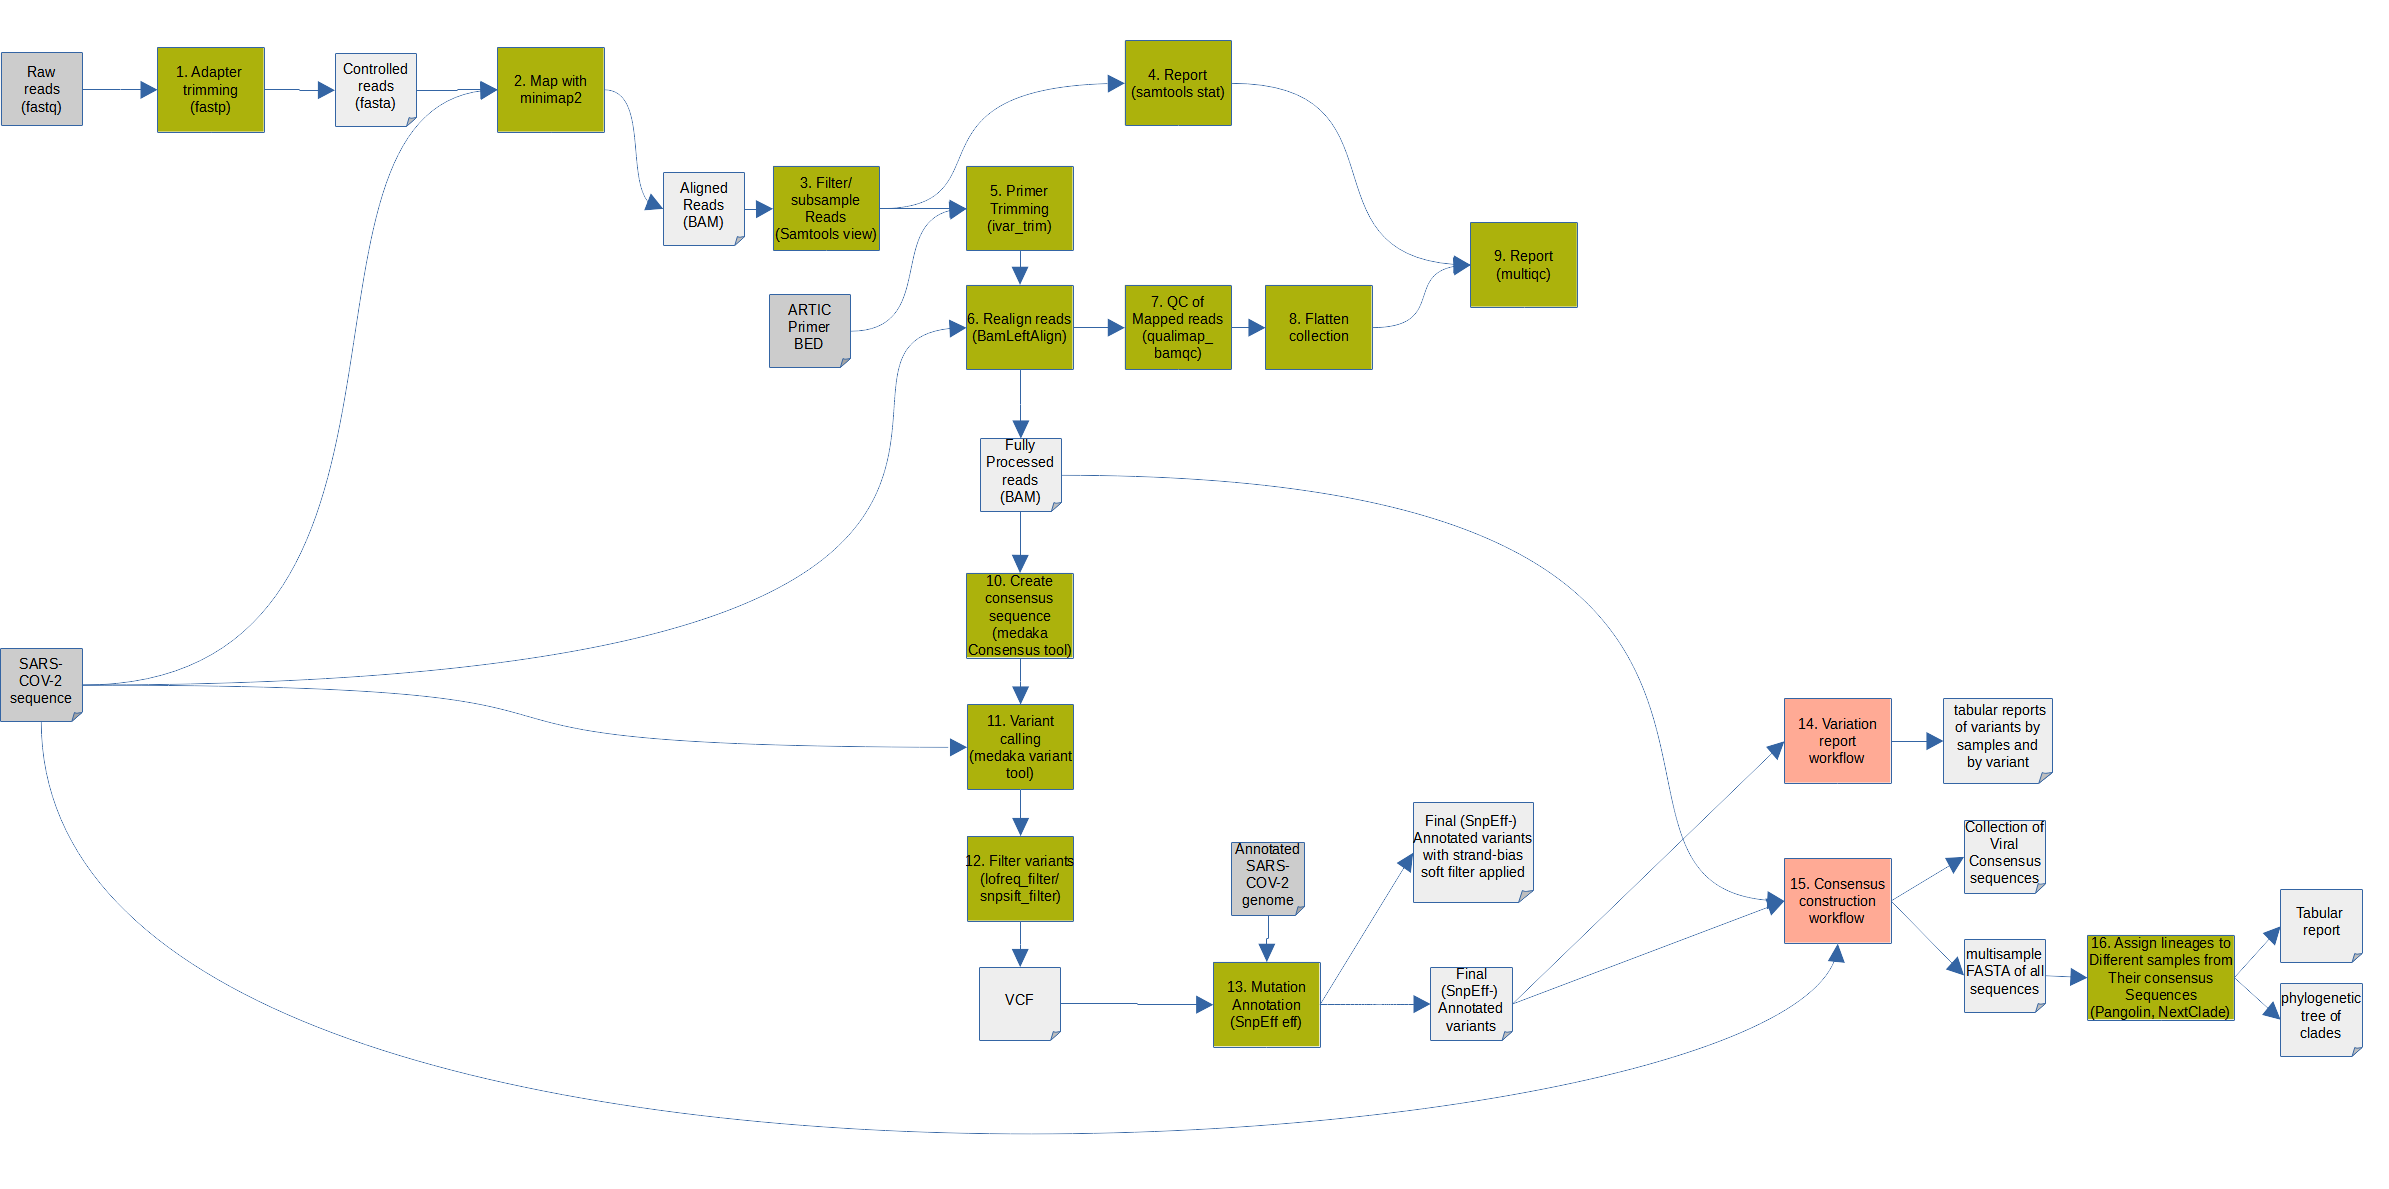
\includegraphics[width=1.4\textwidth]{figures/further/further-ont-wf.png}
            \captionof{figure}{One of four existing Galaxy workflow for SARS-CoV-2 clinical data surveillance for single-end reads data extracted with amplicon-based technique and sequenced with Nanopore sequencing approach.}
            \label{fig:further:ont-wf}
        \end{figure}
        \begin{figure}[ht!]
        	\centering
            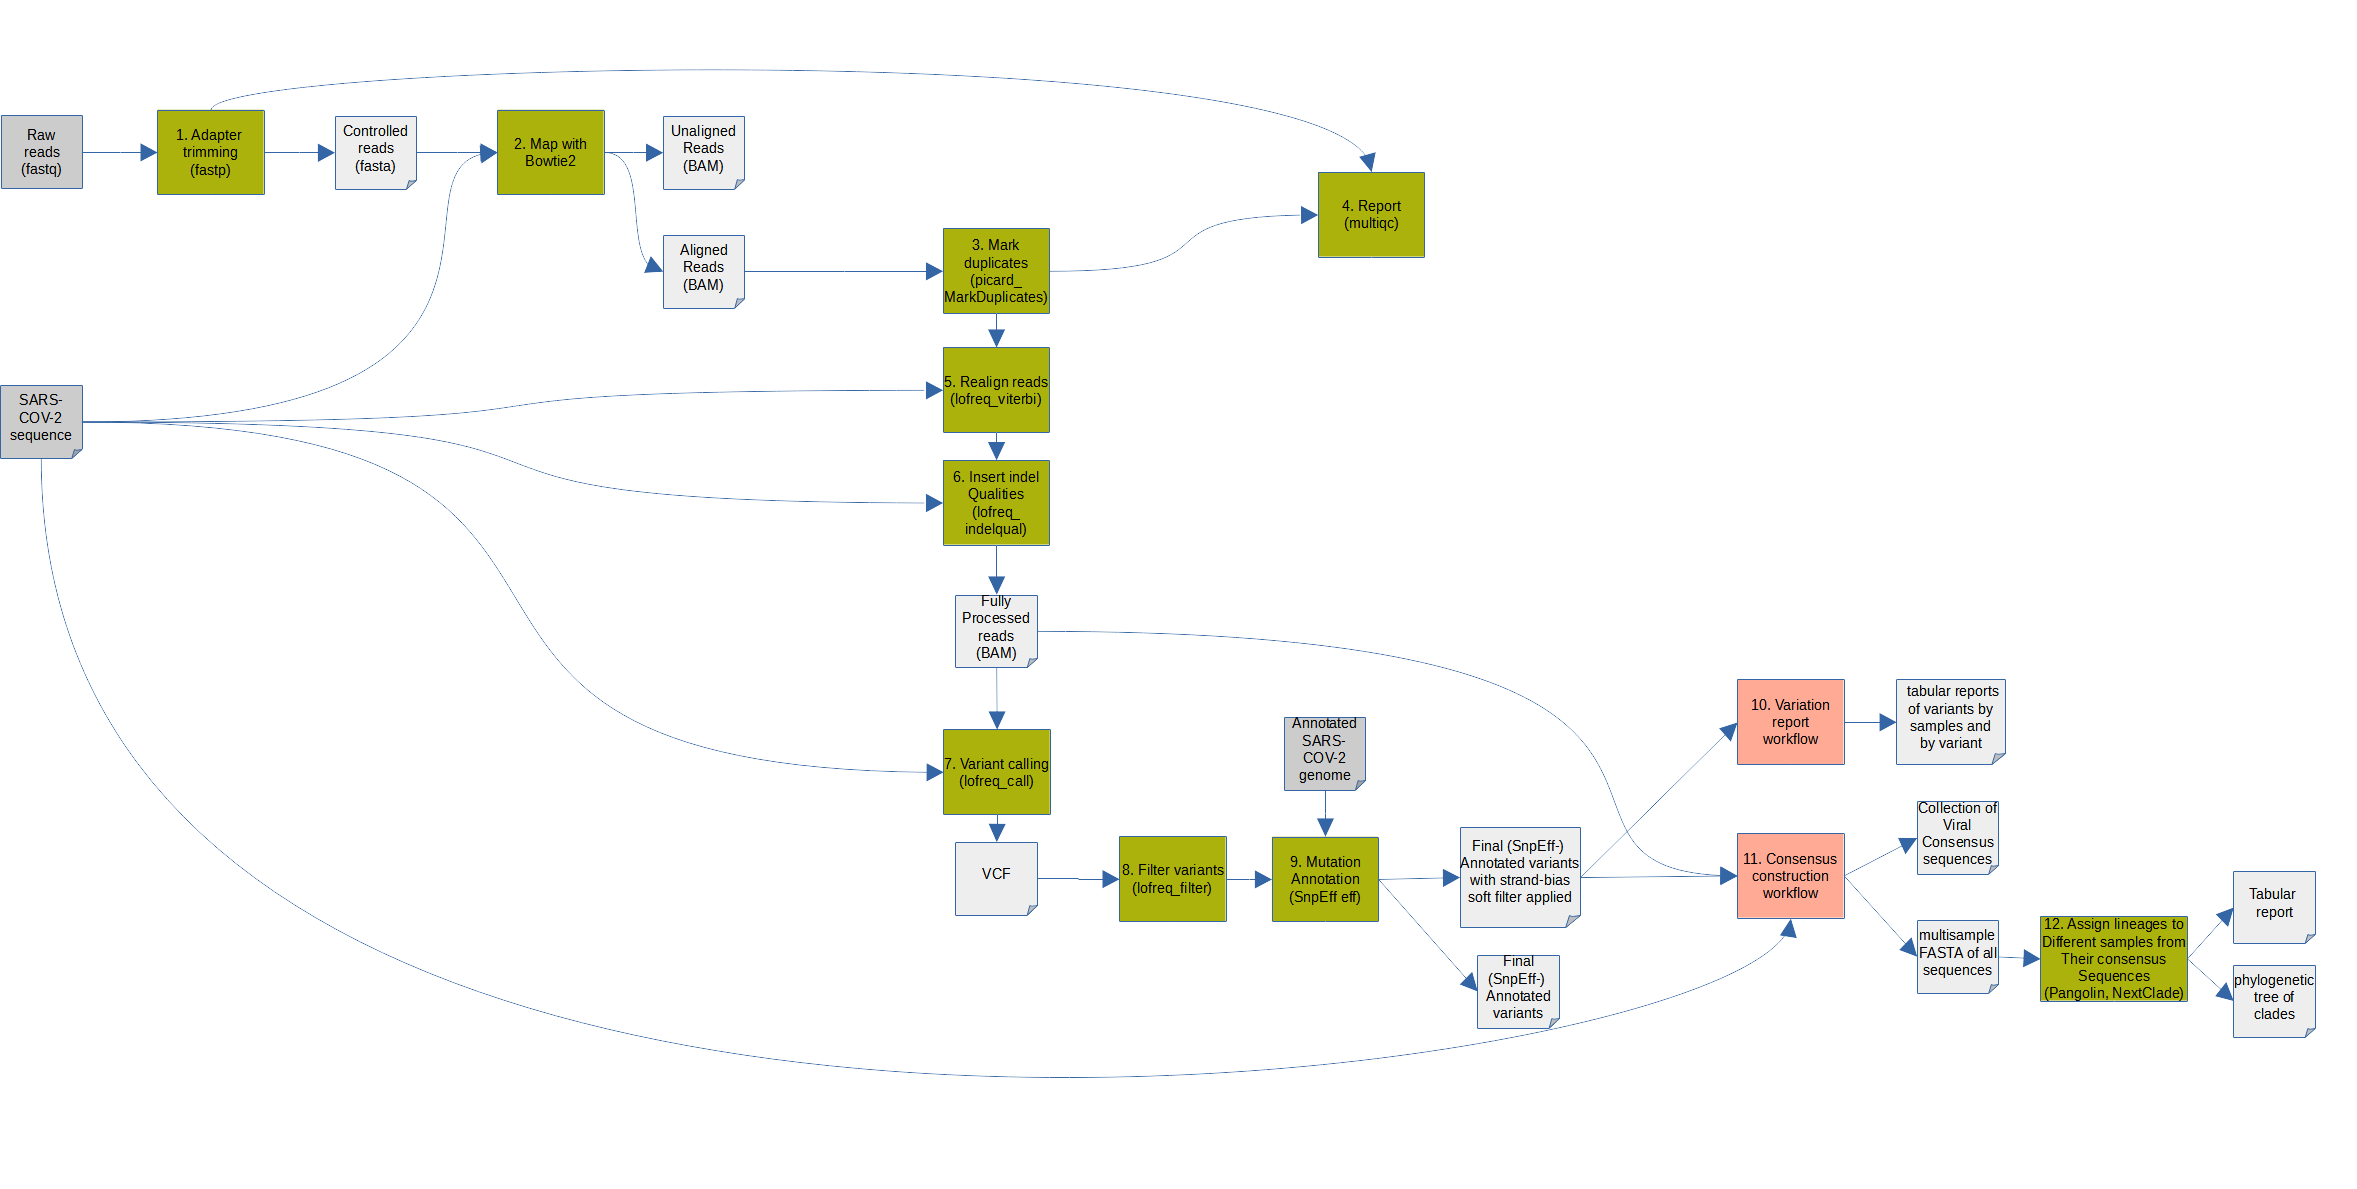
\includegraphics[width=1.4\textwidth]{figures/further/further-illumina-wf.png}
            \captionof{figure}{One of four existing Galaxy workflow for SARS-CoV-2 clinical data surveillance for single-end reads data extracted with metatranscriptomic-based technique and sequenced with Illumina sequencing approach.}
            \label{fig:further:illumina-wf}
        \end{figure}
        \vfill
        \end{landscape}
        
        \subsubsection{Parallel coordinates} 
        \paragraph{Parallel coordinates for all mock samples} \label{sec:appendix:figures:parallel-all}
        \Cref{fig:further:parallel-delta-all}, \cref{fig:further:parallel-ba1-all} and \cref{fig:further:parallel-ba2-all} depict parallel coordinates for all samples considering only detection of Delta, BA.1, and BA.2 lineage respectively by Freyja and COJAC.
        \begin{figure}[H]
        	\centering
            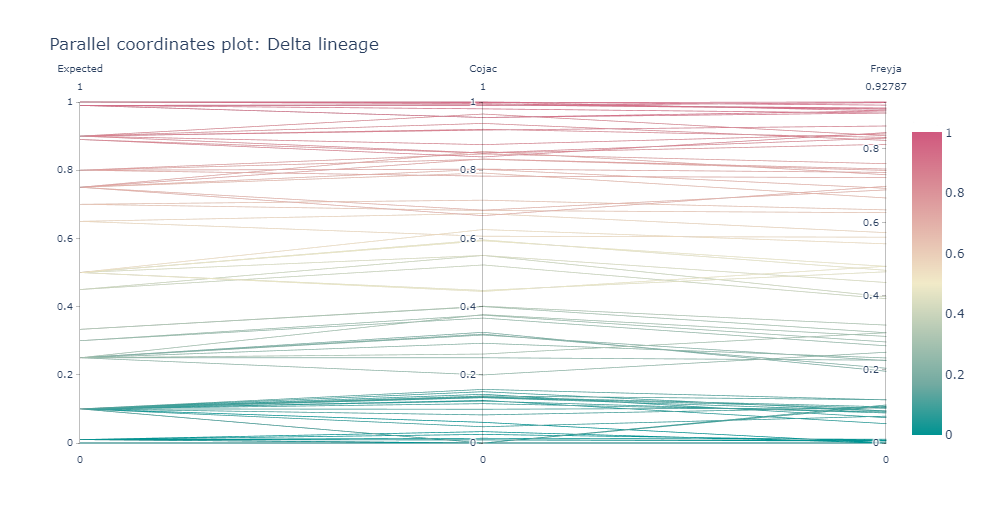
\includegraphics[width=0.8\textwidth]{figures/further/pc-delta-all.png}
            \captionof{figure}{Parallel coordinates plot for all samples that compare Delta lineage proportions detected by Freyja and COJAC with each other as well as with expected proportion. Left axis represents expected proportion of Delta, middle axis represents proportion of Delta lineage detected by COJAC, while right axis represents proportion of Delta lineage detected by Freyja}
            \label{fig:further:parallel-delta-all}
        \end{figure}
        \begin{figure}[H]
        	\centering
            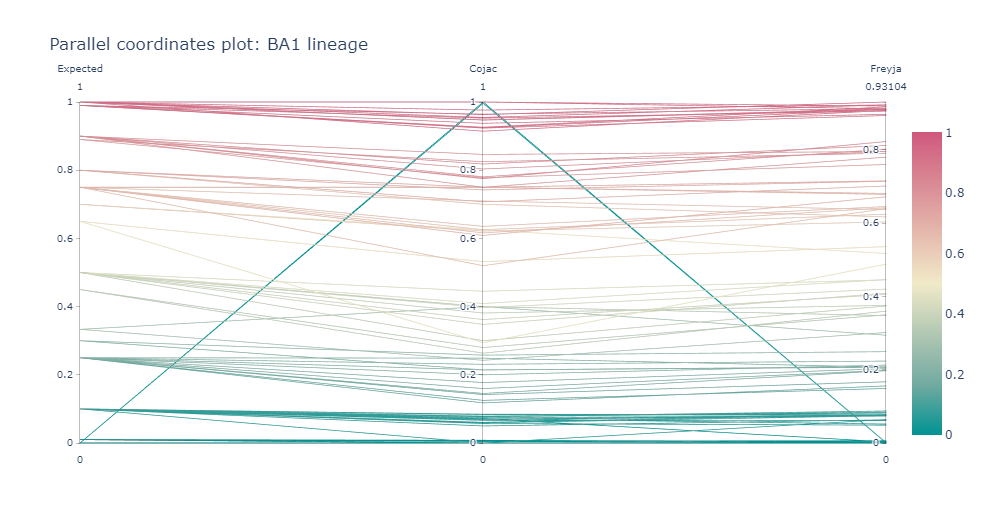
\includegraphics[width=0.8\textwidth]{figures/further/pc-ba1-all.png}
            \captionof{figure}{Parallel coordinates plot for all samples that compare BA.1 lineage proportions detected by Freyja and COJAC with each other as well as with expected proportion. Left axis represents expected proportion of BA.1, middle axis represents proportion of BA.1 lineage detected by COJAC, while right axis represents proportion of BA.1 lineage detected by Freyja}
            \label{fig:further:parallel-ba1-all}
        \end{figure}
        \begin{figure}[H]
        	\centering
            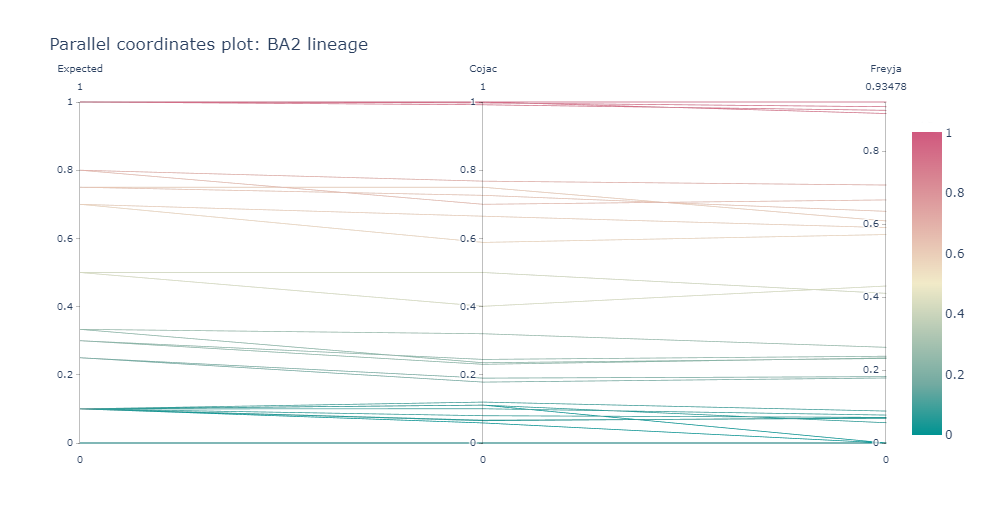
\includegraphics[width=0.8\textwidth]{figures/further/pc-ba2-all.png}
            \captionof{figure}{Parallel coordinates plot for all samples that compare BA.2 lineage proportions detected by Freyja and COJAC with each other as well as with expected proportion. Left axis represents expected proportion of BA.2, middle axis represents proportion of BA.2 lineage detected by COJAC, while right axis represents proportion of BA.2 lineage detected by Freyja}
            \label{fig:further:parallel-ba2-all}
        \end{figure}
        
        \paragraph{Parallel coordinates for mock samples with two lineages expected} \label{sec:appendix:figures:parallel-twolin}
        \Cref{fig:further:parallel-delta-twolin}, \cref{fig:further:parallel-ba1-twolin} and \cref{fig:further:parallel-ba2-twolin} depict parallel coordinates for "two lineages" group of samples considering only detection of Delta, BA.1, and BA.2 lineage respectively by Freyja and COJAC. Although, for the "two lineages" group of samples, it is not that reasonable to separate graphs into different lineages but focus on the ratio between two expected lineages. Even though, detected proportion of certain expected lineage was worthwhile to to have a look at. Thus, parallel coordinates graphs were generated in the way of one graph per lineage.
        \begin{figure}[H]
        	\centering
            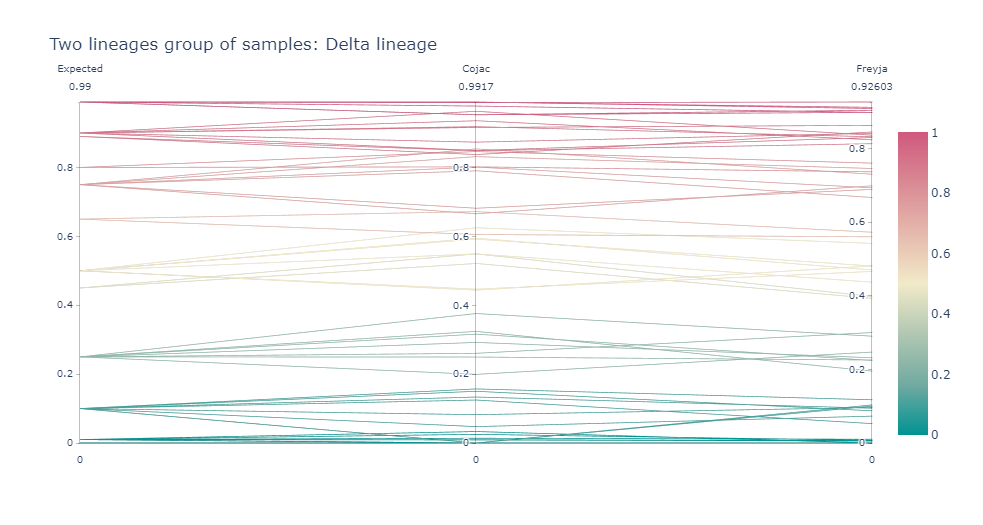
\includegraphics[width=0.8\textwidth]{figures/further/pc-twolin-delta.png}
            \captionof{figure}{Parallel coordinates plot for "two lineages group" of samples that compare Delta lineage proportions detected by Freyja and COJAC with each other as well as with expected proportion. Left axis represents expected proportion of Delta, middle axis represents proportion of Delta lineage detected by COJAC, while right axis represents proportion of Delta lineage detected by Freyja}
            \label{fig:further:parallel-delta-twolin}
        \end{figure}
        \begin{figure}[H]
        	\centering
            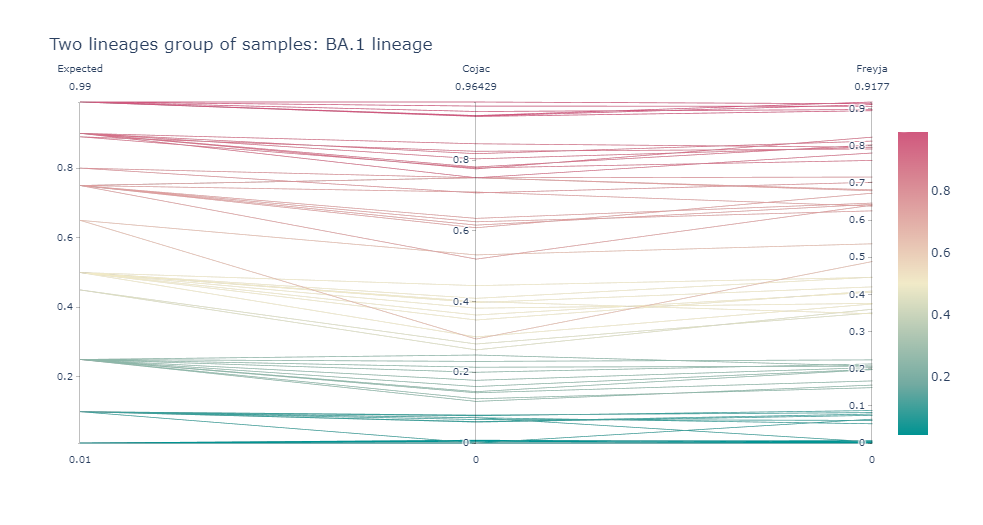
\includegraphics[width=0.8\textwidth]{figures/further/pc-twolin-ba1.png}
            \captionof{figure}{Parallel coordinates plot for "two lineages group" of samples that compare BA.1 lineage proportions detected by Freyja and COJAC with each other as well as with expected proportionfor "two lineages group" of samples. Left axis represents expected proportion of BA.1, middle axis represents proportion of BA.1 lineage detected by COJAC, while right axis represents proportion of BA.1 lineage detected by Freyja}
            \label{fig:further:parallel-ba1-twolin}
        \end{figure}
        \begin{figure}[H]
        	\centering
            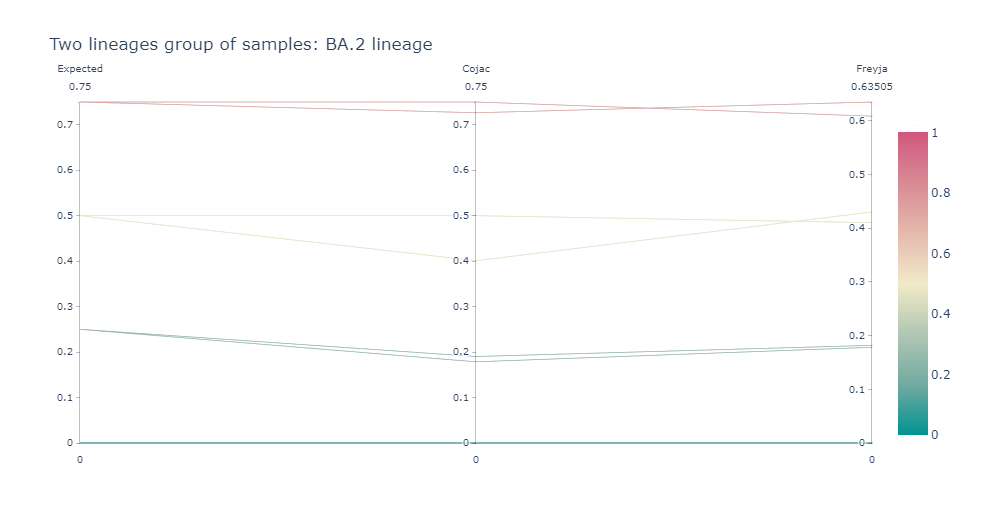
\includegraphics[width=0.8\textwidth]{figures/further/pc-twolin-ba2.png}
            \captionof{figure}{Parallel coordinates plot for "two lineages group" of samples that compare BA.2 lineage proportions detected by Freyja and COJAC with each other as well as with expected proportion for "two lineages group" of samples. Left axis represents expected proportion of BA.2, middle axis represents proportion of BA.2 lineage detected by COJAC, while right axis represents proportion of BA.2 lineage detected by Freyja}
            \label{fig:further:parallel-ba2-twolin}
        \end{figure}
        
        \subsubsection{Example of different types of plots for one mock sample} 
        \Cref{fig:further:bar-s1}, \cref{fig:further:pc-s1} and \cref{fig:further:line-s1} show plots generated per sample to make detailed observations. The example for the sample1 is provided below. However, these graphs were constructed for every sample during this master thesis. Types of plots that were generated per one sample: i) bar plot (\cref{fig:further:bar-s1}); ii) parallel coordinates plot (\cref{fig:further:pc-s1}); iii) line plot (\cref{fig:further:line-s1}), to look at absolute values of lineage proportion against scaled values in parallel coordinates. The comparison with expected lineage proportions was included in these plots.
.
        \begin{figure}[H]
        	\centering
            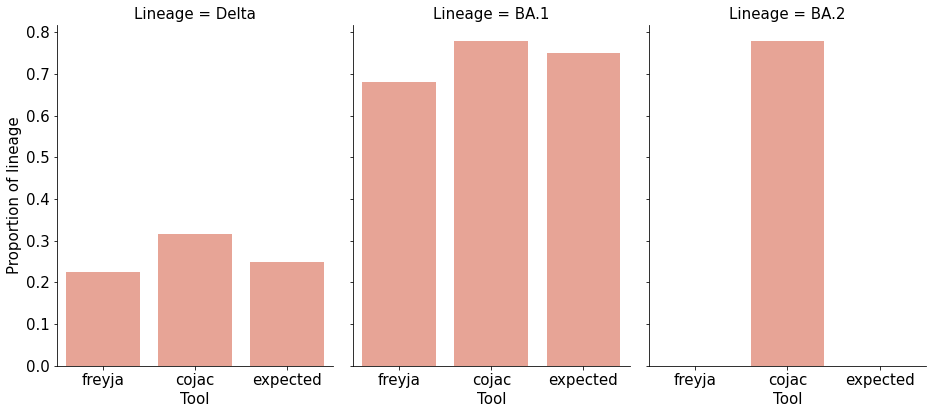
\includegraphics[width=0.8\textwidth]{figures/further/bar-s1.png}
            \captionof{figure}{Bar plot for sample 1.}
            \label{fig:further:bar-s1}
        \end{figure}
        \begin{figure}[H]
        	\centering
            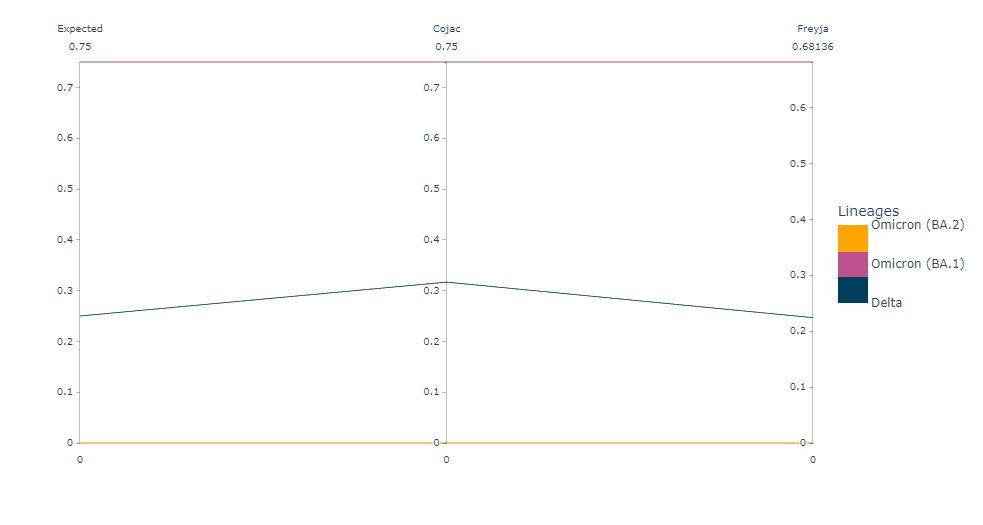
\includegraphics[width=0.8\textwidth]{figures/further/pc-s1.png}
            \captionof{figure}{Parallel coordinates plot for sample 1}
            \label{fig:further:pc-s1}
        \end{figure}
        \begin{figure}[H]
        	\centering
            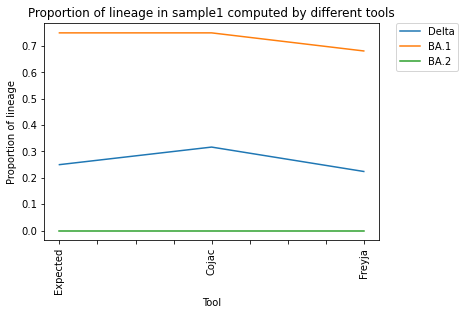
\includegraphics[width=0.8\textwidth]{figures/further/line-s1.png}
            \captionof{figure}{Line plot for sample 1}
            \label{fig:further:line-s1}
        \end{figure}
        
        \subsubsection{Collection of bar plots across all mock samples} \label{sec:appendix:figures:bars-all}
        \Cref{fig:further:bars-delta-all}, \cref{fig:further:bars-ba1-all} and \cref{fig:further:bars-ba2-all} depict barplots for all samples considering only detection of Delta, BA.1, and BA.2 lineage respectively.
        
        \begin{figure}[H]
        	\centering
            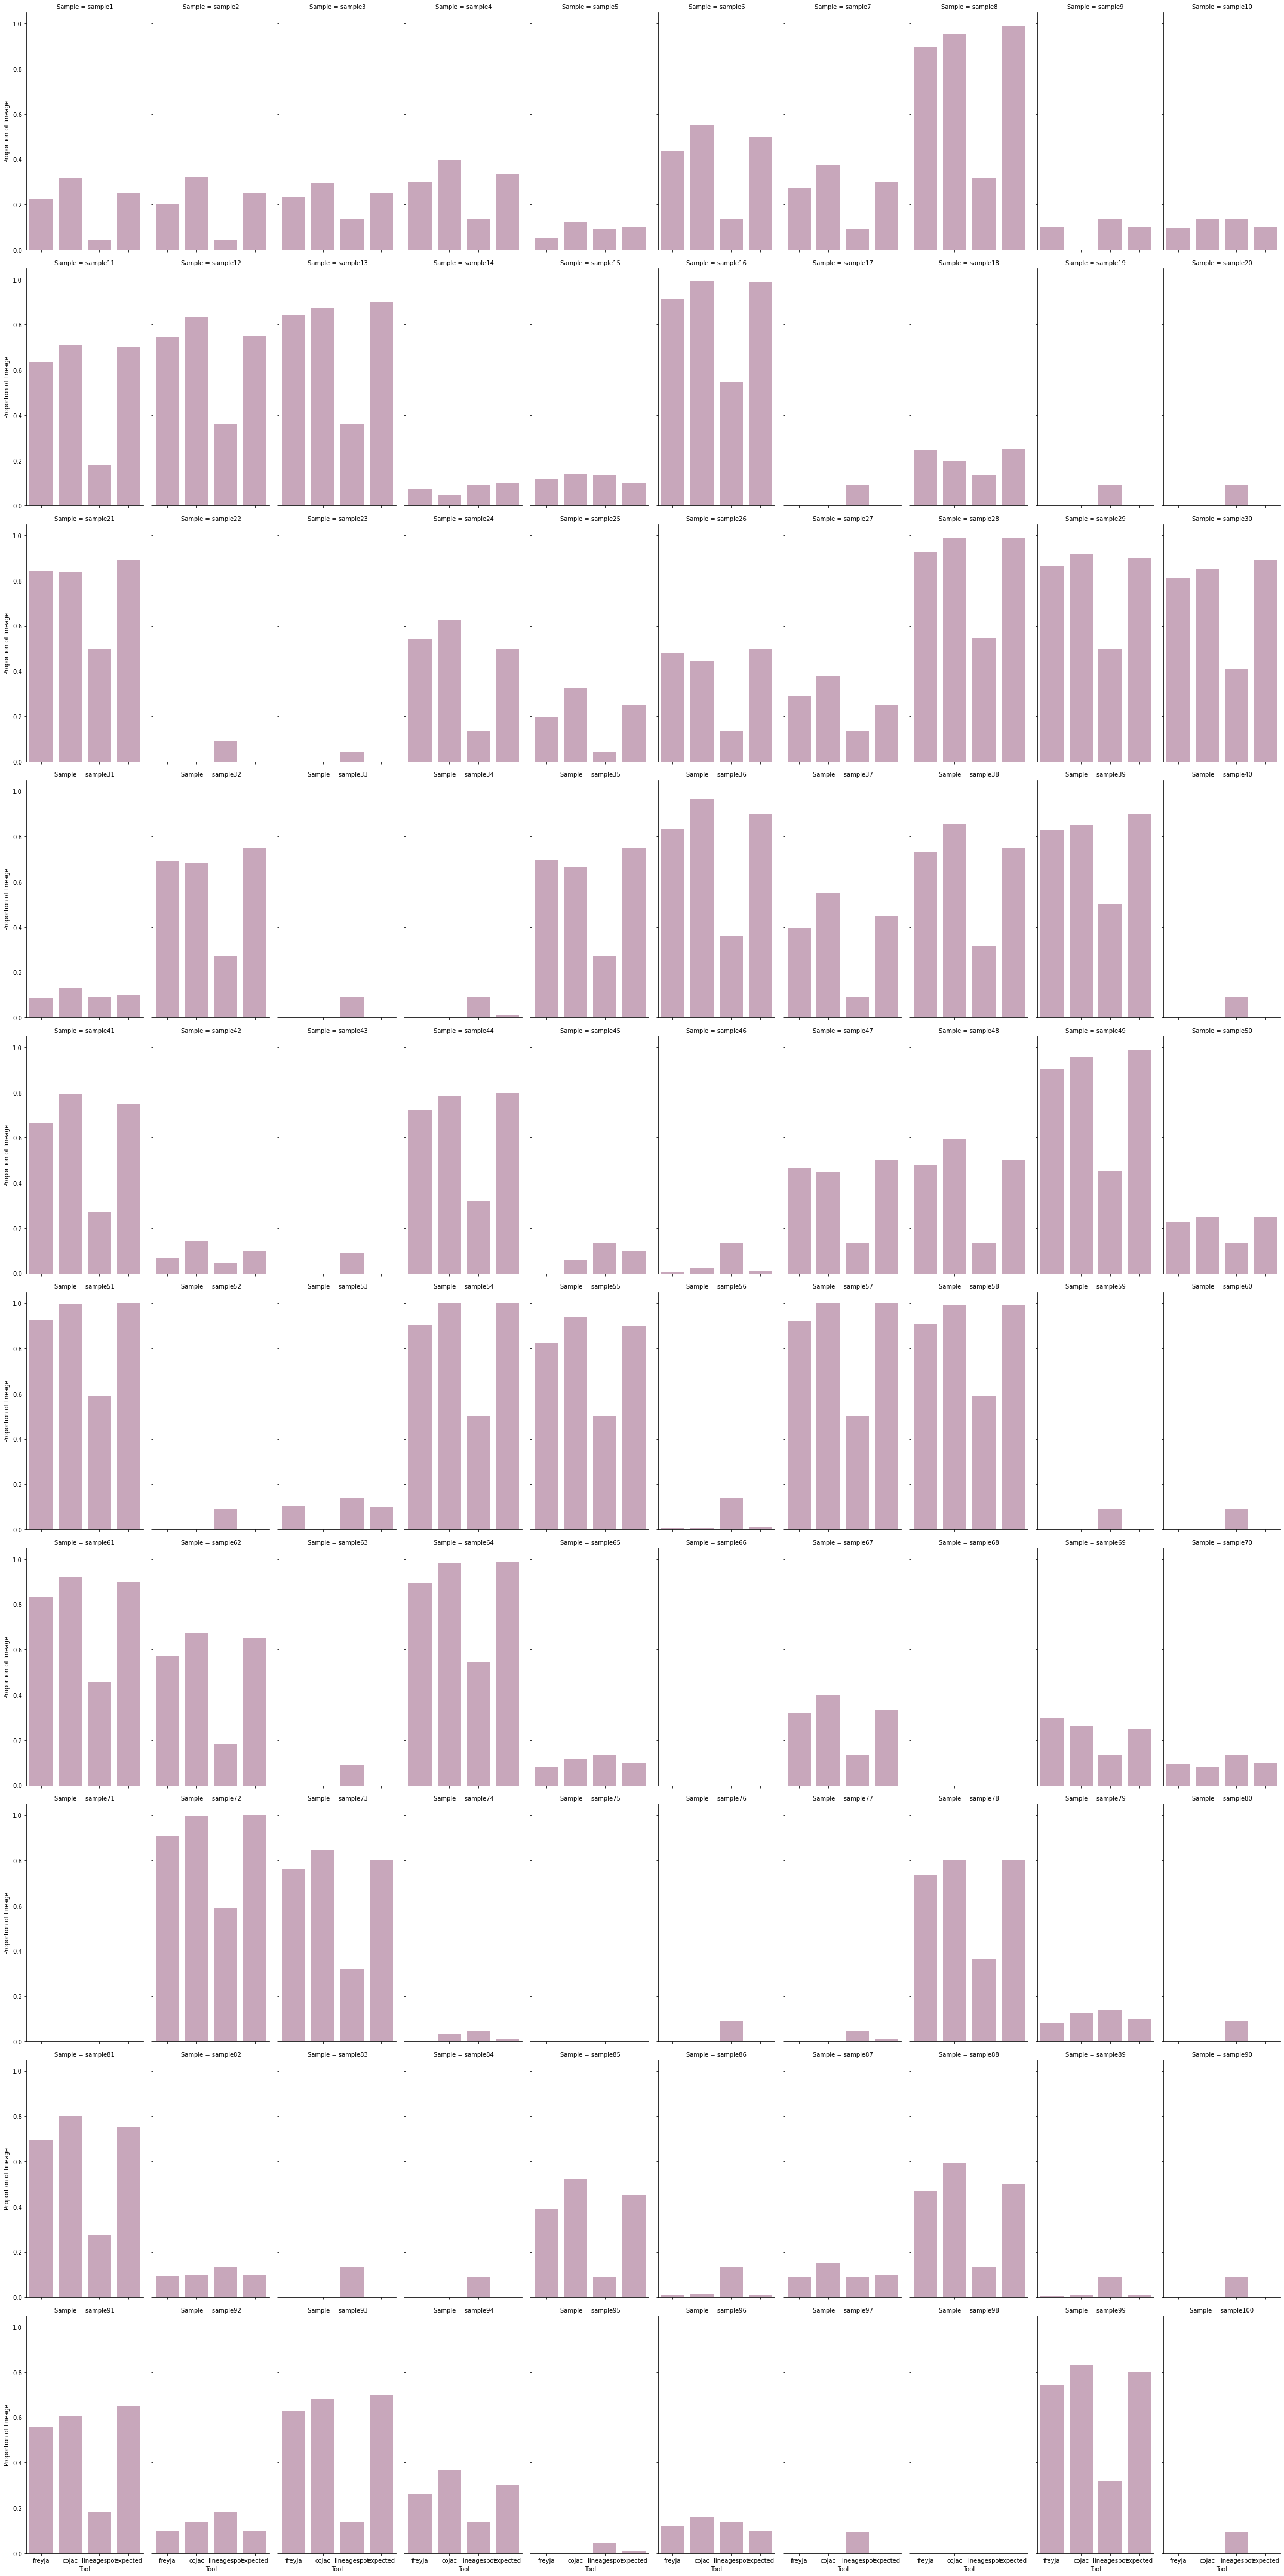
\includegraphics[width=0.7\textwidth]{figures/further/bars-delta-all.png}
            \captionof{figure}{Bar plots that compare Delta lineage proportions detected by Freyja and COJAC with each other as well as with expected proportion.}
            \label{fig:further:bars-delta-all}
        \end{figure}
        \begin{figure}[H]
        	\centering
            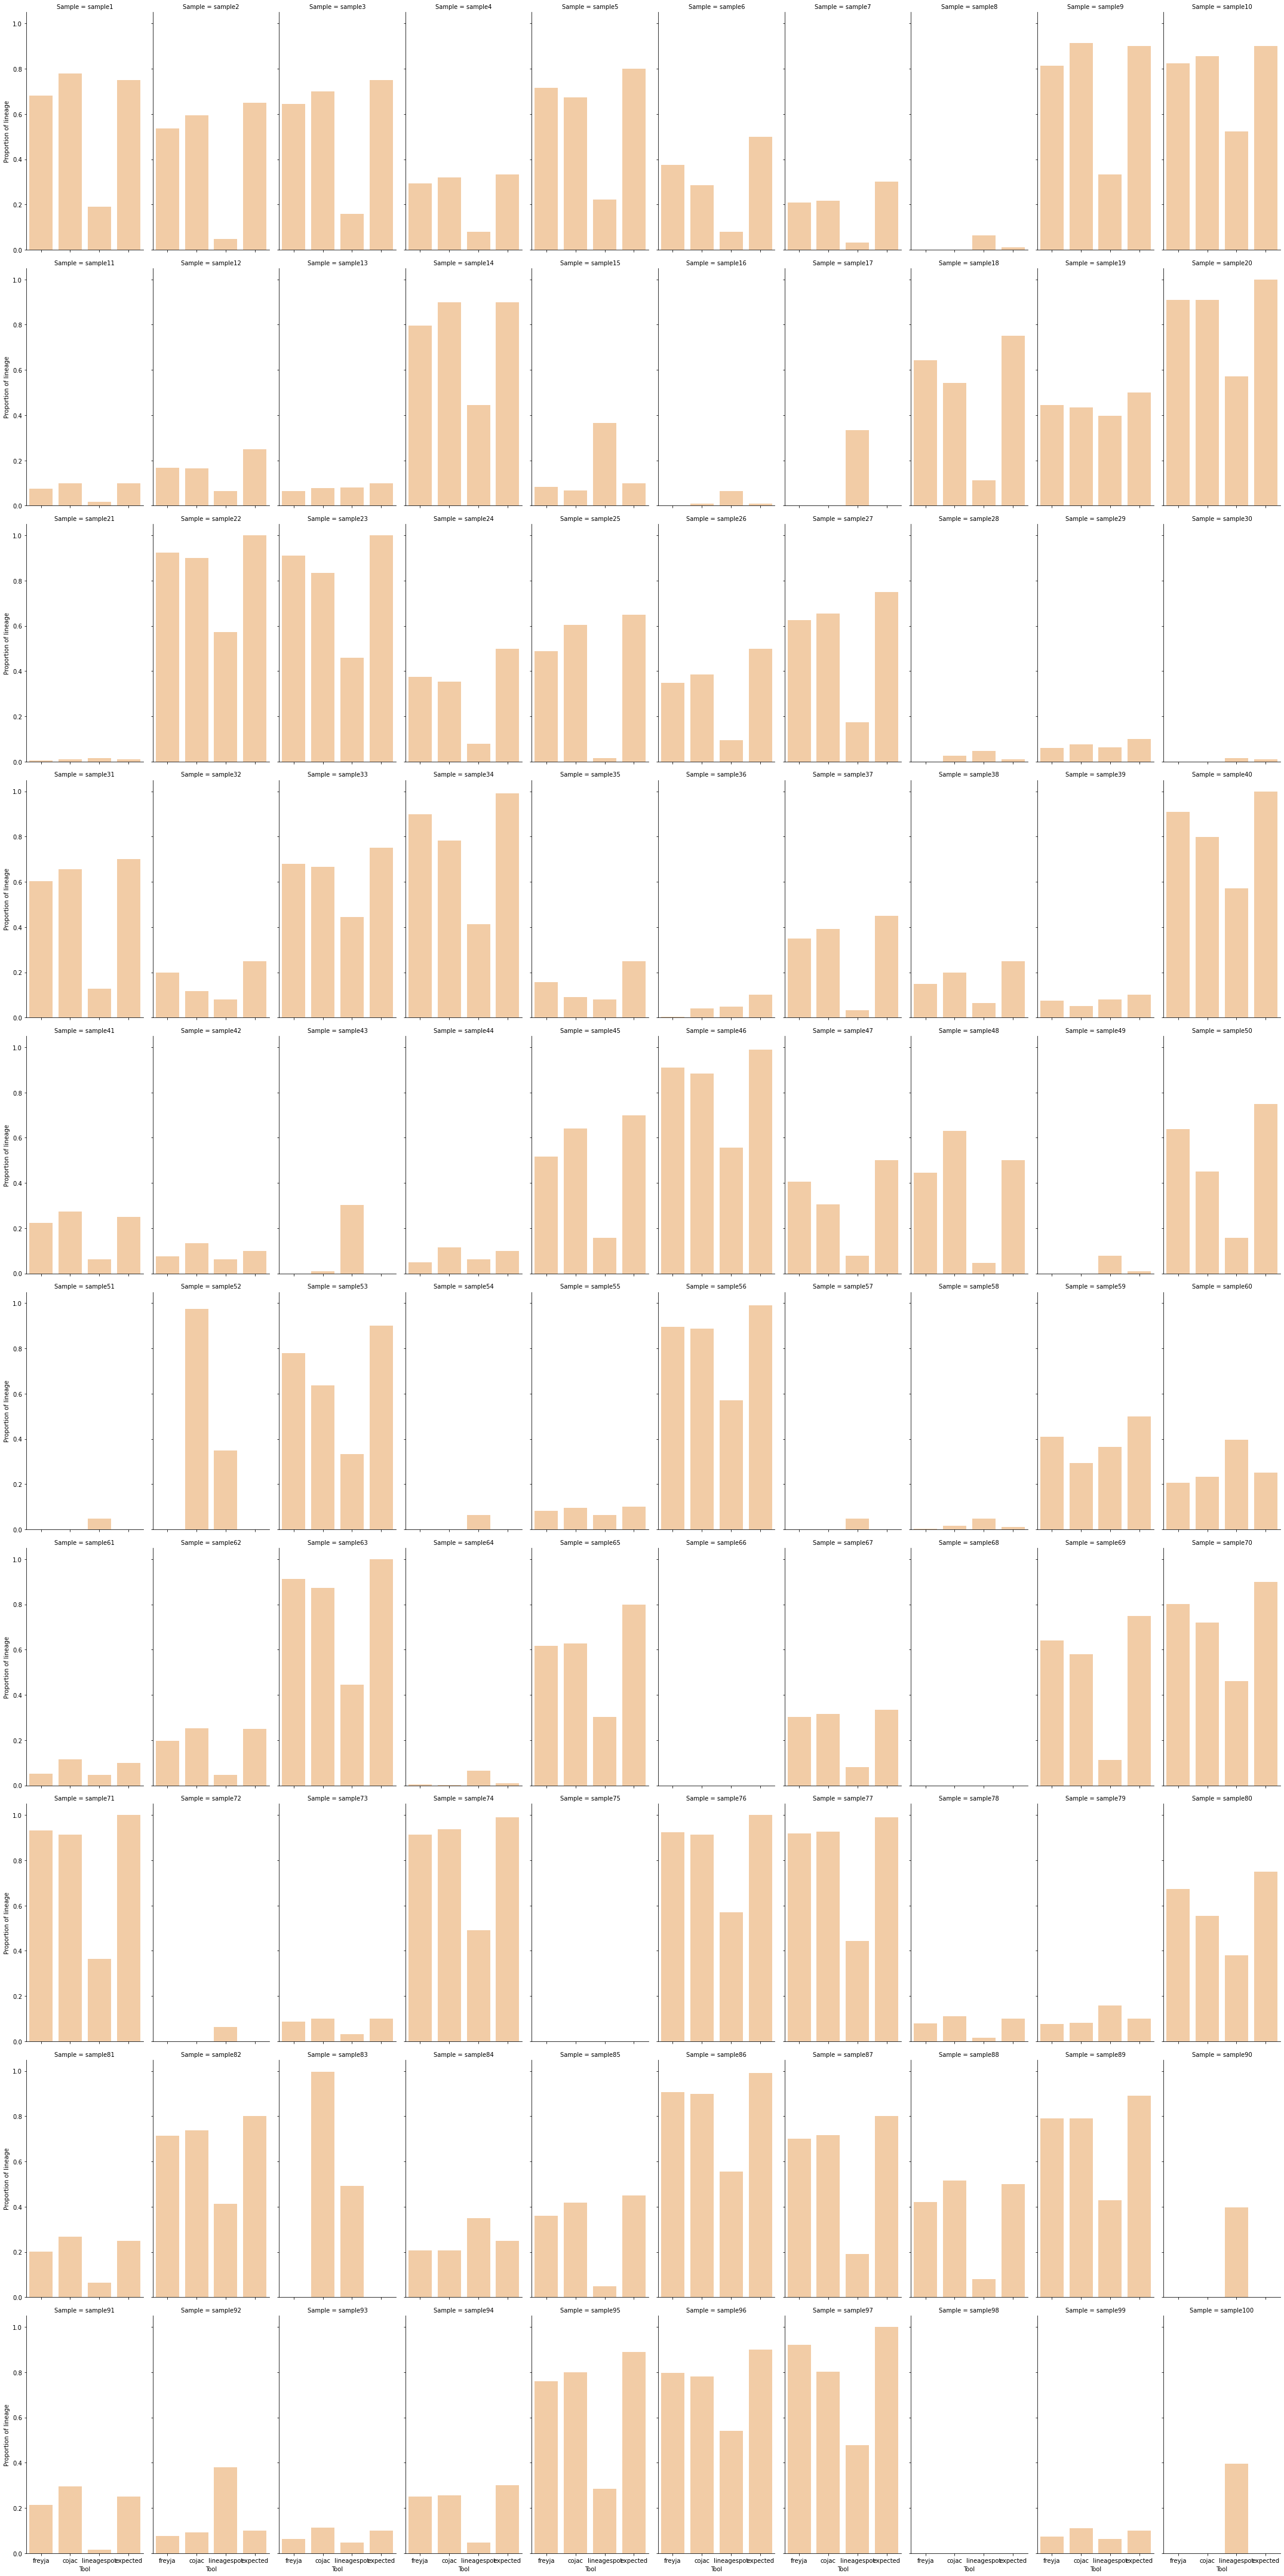
\includegraphics[width=0.7\textwidth]{figures/further/bars-ba1-all.png}
            \captionof{figure}{Bar plots that compare BA.1 lineage proportions detected by Freyja and COJAC with each other as well as with expected proportion}
            \label{fig:further:bars-ba1-all}
        \end{figure}
        \begin{figure}[H]
        	\centering
            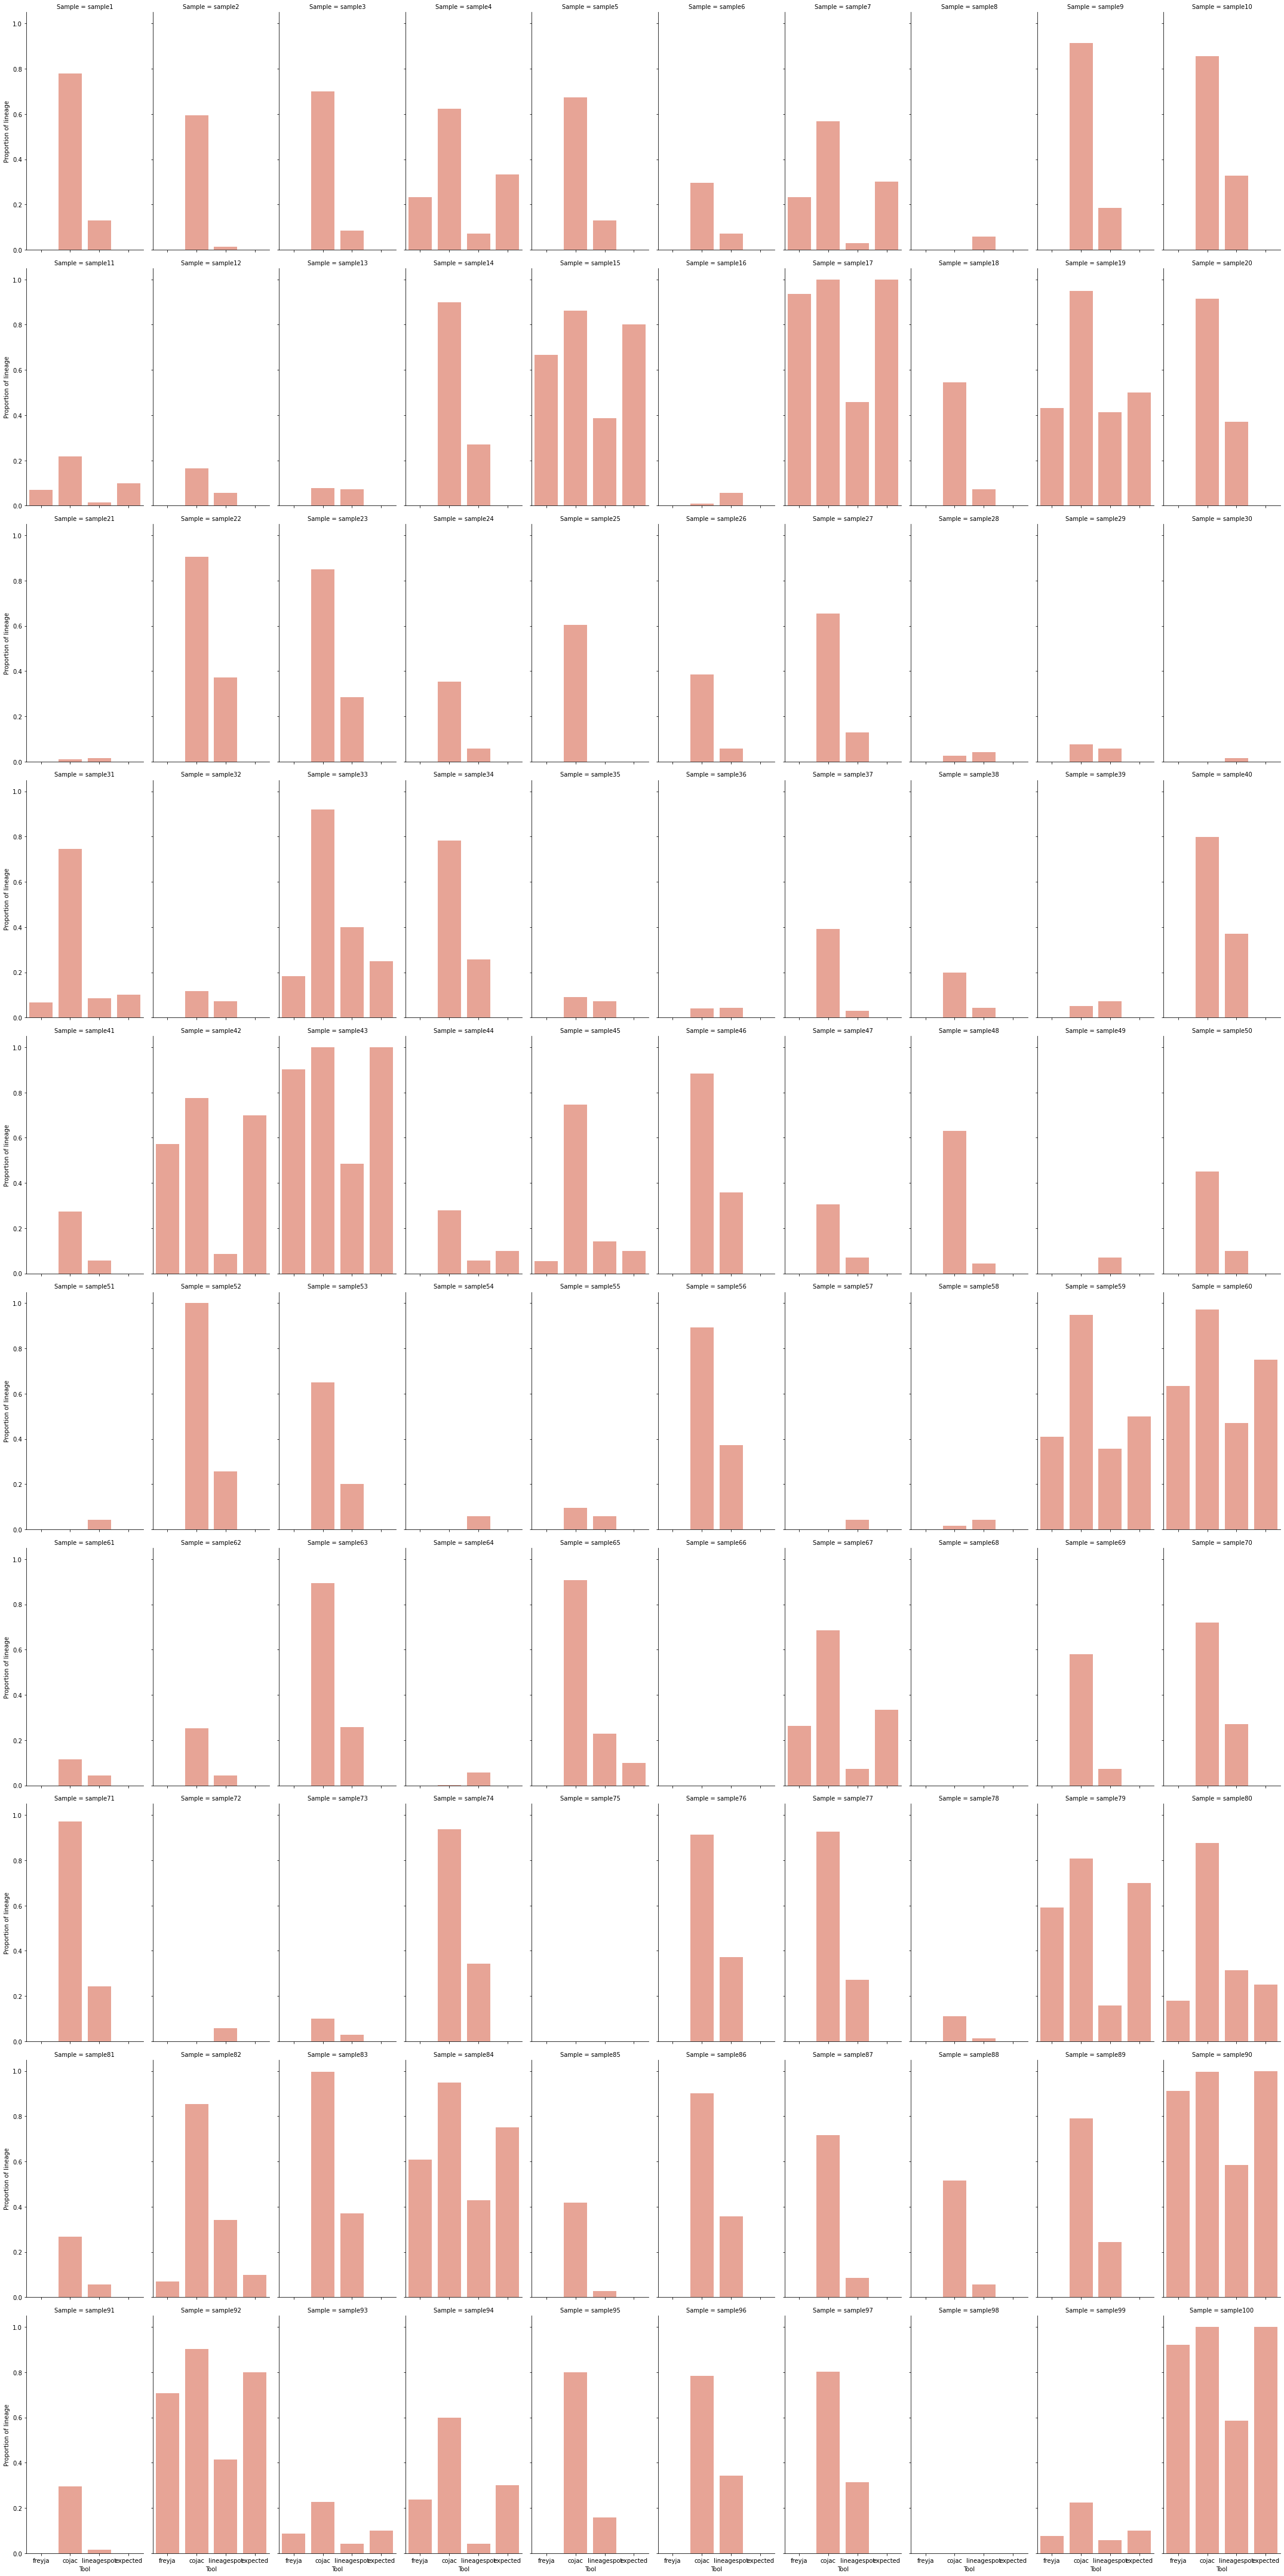
\includegraphics[width=0.7\textwidth]{figures/further/bars-ba2-all.png}
            \captionof{figure}{Bar plots that compare BA.2 lineage proportions detected by Freyja and COJAC with each other as well as with expected proportion.}
            \label{fig:further:bars-ba2-all}
        \end{figure}
        
       \subsubsection{Distribution of lineages proportions detected by Lineagespot across all mock samples}  
        \Cref{fig:further:dist-ls} represents the proportions of every lineage detected by Lineagespot on mock dataset. Observed that most of the samples, more than 50\%, according to Lineagespot, carry a small proportion, no more than 0.15, of lineage abundance, while higher proportions of all 3 lineages are present in less amount of samples.
        \begin{figure}[H]
        	\centering
            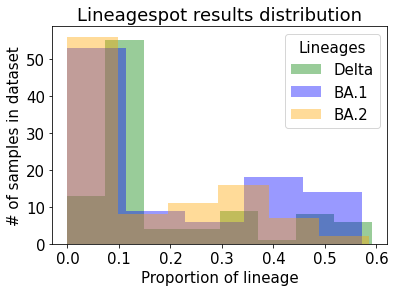
\includegraphics[width=0.5\textwidth]{figures/further/distr-lineagespot.png}
            \captionof{figure}{All three considered lineages (Delta, BA.1, BA.2) proportion distribution among results detected by Lineagespot on mock dataset.}
            \label{fig:further:dist-ls}
        \end{figure}
        
    \subsection{Supplementary tables}
        \subsubsection{Freyja aggregated demixed data} \label{sec:appendix:tabs:freyja}
\begin{landscape}
            \centering\vspace*{\fill}
                \begin{table}[ht!]
                \tiny
                \begin{tabular}{l|l|l|l|l|l}
                            &summarized&lineages&abundances&resid&coverage\\ \hline
                SRR12596165.fastq&"[('Other', 0.9999999999972105)]"&\multicolumn{1}{m{5cm}|}{B.10 B.47 B.23 B.26 B.1.14 B.20 B}&\multicolumn{1}{m{5cm}|}{0.14285714 0.14285714 0.14285714 0.14285714 0.14285714 0.14285714 0.14285714}&2.63E-12&1.926550271\\ \hline
                SRR12596166.fastq&"[('Other', 0.9999999999983175)]"&\multicolumn{1}{m{5cm}|}{B.1.1.174 B.10 B.47 B.23 B.26 B.1.14 B.20 B}&\multicolumn{1}{m{5cm}|}{0.55555600 0.06349200 0.06349200 0.06349200 0.06349200 0.06349200 0.06349200 0.06349200}&1.162673375&1.926550271\\ \hline
                SRR12596167.fastq&"[('Other', 0.9999999999996593)]"&\multicolumn{1}{m{5cm}|}{B.10 B.47 B.23 B.26 B.1.14 B.20 B}&\multicolumn{1}{m{5cm}|}{0.14285714 0.14285714 0.14285714 0.14285714 0.14285714 0.14285714 0.14285714}&0.75&1.926550271\\ \hline
                SRR12596168.fastq&"[('Other', 0.9999999999582964)]"&\multicolumn{1}{m{5cm}|}{B.1.1.174 B.1.1.161 B.1.564 B.1.12 B.1.607 B.1.413 B.1.324 B.1.453 B.1.1.372 B.1.1 B.1.1.92 B.1.1.294 B.1.1.180 B.1.1.43 B.1.1.59 B.1.1.463 B.1.1.402 B.1.1.10 B.1.1.208 B.1.1.61 B.10 B.47 B.23 B.26 B.1.14 B.20 B}&\multicolumn{1}{m{5cm}|}{0.27027000 0.08080800 0.05555550 0.05555550 0.05555550 0.05555550 0.05555550 0.05555550 0.02377383 0.02377383 0.02377383 0.02377383 0.02377383 0.02377383 0.02377383 0.02377383 0.02377383 0.02377383 0.02377383 0.02377383 0.00432900 0.00432900 0.00432900 0.00432900 0.00432900 0.00432900 0.00432900}&0.4968557797&1.926550271\\ \hline
                SRR12596169.fastq&"[('Other', 0.9999999999979102)]"&\multicolumn{1}{m{5cm}|}{B.1.111 B.1.1.174 B.1.479 B.1.22 B.1.533 B.1.12 B.1.607 B.1.453 B.1.324 B.1.413 B.1.564 B.1.199 B.1.378 B.1.201 B.1.215 B.1}&\multicolumn{1}{m{5cm}|}{0.14432305 0.14285700 0.09853229 0.06999717 0.05158700 0.04640292 0.04640292 0.04640292 0.04640292 0.04640292 0.04640292 0.04285720 0.04285720 0.04285720 0.04285720 0.04285720}&0.7140985235&1.926550271\\ \hline
                SRR12596170.fastq&"[('Other', 0.9999999999987905)]"&\multicolumn{1}{m{5cm}|}{B.1.533 B.1.370 B.1.301 B.1.424 B.1.111 B.1.479 B.1.201 B.1.378 B.1.199 B.1.215 B.1 B.1.22 B.1.453 B.1.324 B.1.413 B.1.607 B.1.12 B.1.564 B.1.1.161 B.10 B.47 B.23 B.26 B.1.14 B.20 B}&\multicolumn{1}{m{5cm}|}{0.15773800 0.11717199 0.11641401 0.11641400 0.05154872 0.03906387 0.03904760 0.03904760 0.03904760 0.03904760 0.03904760 0.03189755 0.01718081 0.01718081 0.01718081 0.01718081 0.01718081 0.01718081 0.00892900 0.00892857 0.00892857 0.00892857 0.00892857 0.00892857 0.00892857 0.00892857}&0.4778312073&1.926550271\\ \hline
                SRR12596171.fastq&"[('Other', 0.9979179208943117)]"&\multicolumn{1}{m{5cm}|}{B.1.509 B.1.12 B.1.607 B.1.453 B.1.324 B.1.413 B.1.564 B.10 B.47 B.23 B.26 B.1.14 B.20 B}&\multicolumn{1}{m{5cm}|}{0.87096800 0.01560282 0.01560282 0.01560282 0.01560282 0.01560282 0.01560282 0.00476186 0.00476186 0.00476186 0.00476186 0.00476186 0.00476186 0.00476186}&0.3834278298&1.926550271\\ \hline
                SRR12596172.fastq&"[('Other', 0.9999999999983878)]"&\multicolumn{1}{m{5cm}|}{B.1.301 B.1.424 B.1.370 B.1.1.174 B.1.453 B.1.12 B.1.607 B.1.324 B.1.413 B.1.564 B.47 B.20 B.1.14 B.26 B.23 B B.10 B.1.533 B.1.111 B.1.22 B.1.479}&\multicolumn{1}{m{5cm}|}{0.27497564 0.27497564 0.27312572 0.03731300 0.01588226 0.01588226 0.01588226 0.01588226 0.01588226 0.01588226 0.00529100 0.00529100 0.00529100 0.00529100 0.00529100 0.00529100 0.00529100 0.00367100 0.00125773 0.00118732 0.00116342}&0.54272957&1.926550271\\ \hline
                SRR12596173.fastq&"[('Other', 0.9999999999972105)]"&\multicolumn{1}{m{5cm}|}{B.10 B.47 B.23 B.26 B.1.14 B.20 B}&\multicolumn{1}{m{5cm}|}{0.14285714 0.14285714 0.14285714 0.14285714 0.14285714 0.14285714 0.14285714}&2.63E-12&1.926550271\\ \hline
                SRR12596174.fastq&"[('Other', 0.999999999979265)]"&\multicolumn{1}{m{5cm}|}{B.1.509 B.1.2 B.1.370 B.1.301 B.1.424 B.1.324 B.1.564 B.1.413 B.1.453 B.1.607 B.1.12 B.1.596 B.47 B.20 B.1.14 B.26 B.23 B B.10 B.1 B.1.215 B.1.201 B.1.378 B.1.199}&\multicolumn{1}{m{5cm}|}{0.28000000 0.20118712 0.06037074 0.06035913 0.06035913 0.04567167 0.04567167 0.04567167 0.04567167 0.04567167 0.04567167 0.02797988 0.00432900 0.00432900 0.00432900 0.00432900 0.00432900 0.00432900 0.00432900 0.00108220 0.00108220 0.00108220 0.00108220 0.00108220}&0.8515939213&1.926550271\\ \hline
                SRR12596175.fastq&"[('Other', 0.9905735237538151)]"&\multicolumn{1}{m{5cm}|}{B.1.509 B.1.2 B.1.382 B.1.111 B.10 B.47 B.23 B.26 B.1.14 B.20 B B.1.479 B.1.22}&\multicolumn{1}{m{5cm}|}{0.68478300 0.27368400 0.00451200 0.00294756 0.00294557 0.00294557 0.00294557 0.00294557 0.00294557 0.00294557 0.00294557 0.00245515 0.00157281}&0.2451972591&1.926550271\\ \hline
                \end{tabular}
                \caption{Aggregated table for Californian real-world dataset (PRJNA661613) - output of 'Freyja: aggregate' tool that aggregate demixed data for all samples in dataset} \label{tab:appendix:freyja}
                \end{table}
                \vfill
            \end{landscape}
        
        
\clearpage



%\cleardoublepage
\printbibliography
\clearpage
\printglossaries

\end{document}
